
%%%%%%%%%%%%%%%%%%%%%%%%%%%%%%%%%%%%
% This is the template for submission to ISCA 2016
% The cls file is a modified from  'sig-alternate.cls'
%%%%%%%%%%%%%%%%%%%%%%%%%%%%%%%%%%%%

\documentclass{sig-alternate}
%\usepackage{mathptmx} % This is Times font

%\newcommand{\ignore}[1]{}
\usepackage{fancyhdr}
\usepackage[normalem]{ulem}
\usepackage[hyphens]{url}
\usepackage{hyperref}

\usepackage{tabularx}
\usepackage{ulem}
%\usepackage{program}


%%%%%%%%%%%%%%%%%%%%%%%%%%%%%%%%%%%%%%%%%%%%%%%%%%
% I need these so it compiles on my Ubuntu machine
% There's some issue with the algorithm2e package
%\makeatletter
%\newif\if@restonecol
%\makeatother
%\let\algorithm\relax
%\let\endalgorithm\relax
%%%%%%%%%%%%%%%%%%%%%%%%%%%%%%%%%%%%%%%%%%%%%%%%%%
\usepackage[boxruled]{algorithm2e}


%\usepackage{algorithm2e}
%\usepackage{mathptmx} % This is Times font

%%%%%%%%%%%---SETME-----%%%%%%%%%%%%%
\newcommand{\microsubmissionnumber}{266}
%%%%%%%%%%%%%%%%%%%%%%%%%%%%%%%%%%%%

\fancypagestyle{firstpage}{
  \fancyhf{}
\setlength{\headheight}{50pt}
\renewcommand{\headrulewidth}{0pt}
  \fancyhead[C]{\normalsize{MICRO 2016 Submission
      \textbf{\#\microsubmissionnumber} -- Confidential Draft -- DO NOT DISTRIBUTE}}
  \pagenumbering{arabic}
}

%%commands
\usepackage{ifthen}
\usepackage{calc}
\usepackage{pifont}
\usepackage{color}
\usepackage{fancyhdr}

\newcounter{hours}
\newcounter{minutes}
\newcommand{\printtime}{%
  \setcounter{hours}{\time/60}%
  \setcounter{minutes}{\time-\value{hours}*60}%
  \thehours:\theminutes}

\newcommand{\myspacing}{1.62}
\newcommand{\linespacing}[1]{\renewcommand{\baselinestretch}{#1}\normalsize}

% Set timeofmake to 'true' to print the time the file was compiled
\newboolean{timeofmake}
\setboolean{timeofmake}{false}


\newcommand{\todo}[1]{{\color{red}\sf\bfseries #1}}
\newcommand{\dontinclude}[1]{ }
\newcommand{\myfootnote}[1]{\footnote{\renewcommand{\baselinestretch}{1.0}\scriptsize #1}}


\newcommand{\putsec}[2]{\vspace{-0.1in}\section{#2}\label{sec:#1}\vspace{-0.0in}}
\newcommand{\putssec}[2]{\vspace{-0.05in}\subsection{#2}\label{ssec:#1}\vspace{-0.0in}}
\newcommand{\putsssec}[2]{\vspace{0.0in}\subsubsection{#2}\label{sssec:#1}\vspace{0.0in}}
\newcommand{\putsssecX}[1]{\vspace{0.0in}\subsubsection*{#1}\vspace{0.0in}}

%\renewcommand{\figurename}{\renewcommand{\baselinestretch}{1.0}\vspace{-0.0in}\footnotesize Figure}
%\renewcommand{\tablename}{\renewcommand{\baselinestretch}{1.0}\vspace{-0.0in}\footnotesize TABLE}
 
\newcommand{\tabput}[3]{
\begin{table}[t]
\renewcommand{\baselinestretch}{0.95}
%\small %also for forcing a baselinestretch update
\begin{center}
{
#2
\vspace{-0.1in}
}
\caption{\footnotesize #3 \label{tab:#1}\vspace{-0.2in}}
\renewcommand{\baselinestretch}{\myspacing}\normalsize
\end{center}
\end{table}
}
  
\newcommand{\tabputW}[3]{
\begin{table*}[h]
\begin{center}
{
#2
}
\end{center}
\caption{\footnotesize #3 \label{tab:#1}}
\end{table*}
}

\newcommand{\figput}[4][1.0\linewidth]{
\begin{figure}[t]
\begin{minipage}{\linewidth}
\footnotesize %also for forcing a baselinestretch update
\begin{center}
\includegraphics[trim=#3, clip, width=#1]{plots/#2}
\end{center}
\vspace{-0.1in}
\caption{\footnotesize #4 \label{fig:#2} \vspace{-0.0in}}
\end{minipage}
\end{figure}
}


\newcommand{\figputW}[4][1.0\linewidth]{
\begin{figure*}
\begin{minipage}{\linewidth}
\footnotesize %also for forcing a baselinestretch update
\begin{center}
\includegraphics[trim=#3, clip, width=#1]{plots/#2}
\end{center}
\vspace{-0.1in}
\caption{\footnotesize #4 \label{fig:#2}}
\end{minipage}
\end{figure*}
}

\newcommand{\figputT}[3]{
\begin{figure}[t]
\begin{minipage}{\linewidth}
\footnotesize %also for forcing a baselinestretch update
\begin{center}
\includegraphics[trim=#2, clip, width=1.0\linewidth]{plots/#1}
\end{center}
\vspace{-0.1in}
\caption{\footnotesize #3 \label{fig:#1}}
\end{minipage}
\end{figure}
}

\newcommand{\figputJ}[4][1.0\linewidth]{
\begin{figure}[htb]
\begin{minipage}{\linewidth}
\footnotesize %also for forcing a baselinestretch update
\begin{center}
\includegraphics[trim=#3, clip, width=#1]{plots/#2}
\end{center}
\caption{\footnotesize #4 \label{fig:#2}}
\end{minipage}
\end{figure}
}

\newcommand{\figref}[1]{Figure~\ref{fig:#1}}
\newcommand{\tabref}[1]{Table~\ref{tab:#1}}
\newcommand{\secref}[1]{Section~\ref{sec:#1}}
\newcommand{\ssecref}[1]{Section~\ref{ssec:#1}}
\newcommand{\sssecref}[1]{Section~\ref{sssec:#1}}

\newcommand{\ignore}[1]{}



\newcommand{\TODO}[1]{\textcolor{red}{\todo{#1}}}
\renewcommand{\arraystretch}{1.5}

%%%%%%%%%%%---SETME-----%%%%%%%%%%%%%
\title {MemPod: A Clustered Architecture for Efficient and Scalable Migration in Flat Address Space Multi-level Memories}
\author{}
%%%%%%%%%%%%%%%%%%%%%%%%%%%%%%%%%%%%

\begin{document}
\maketitle
\thispagestyle{firstpage}
\pagestyle{plain}

\begin{abstract}

In the near future die-stacked DRAM will be present alongside off-chip memories in hybrid memory systems. A large body of recent research has explored possible uses and performance-improving mechanisms regarding such a memory configuration. The first approach is to use this new memory as a last level cache and it has been shown to be beneficial for system performance. Another approach is to use the on-chip memory as an extension of the off-chip one in a ``flat address space'' configuration, exposing more memory capacity to applications leading to performance improvement under capacity constrained workloads.

Research has addressed optimization of flat-address-space memories by optimally placing ``hot page'' in the faster memory. Software managed schemes have high overheads and are coarse grained and hence slow to adapt to changes in application phases. Recently proposed hardware man- ged schemes operate at finer granularity than software by either using simple cache like demand driven placement or using a centralized fixed mapping scheme. The former does not consider hotness of data, whereas the latter will not scale to large memories due to its centralized approach.

In this paper we propose MemPod, a scalable and efficient memory management mechanism for flat address space hybrid memories. MemPod monitors main memory activity and upon predefined intervals migrates the most frequently accessed memory pages to the faster on-chip memory. We propose a novel architectural organization and the use of ``Majority Element Algorithm'' for activity tracking. 

Our results with multi-programmed workloads show MemPod to improve Average Main Memory Time (AMMT) by up to 29\% and 11\% on average compared to the state-of-the-art, while our analysis shows that MemPod is the most viable option compared to the state of the art, as memories become faster in the future. MemPod's novel activity tracking approach leads to significant cost reduction ($\sim$6000x lower storage space requirements) and incredible improvement on future prediction accuracy (58\% average improvement) over traditionally used full counters. 

\end{abstract}

\noindent \textbf{Keywords:} Memory architecture, Die-stacked memory

% !TEX root = ../MemPod.tex
\section{Introduction}
\label{sec:Introduction}

%The memory wall problem has been known to impede system performance \cite{wulf-can95}. 3D stacked memory is considered as a viable solution and has been studied extensively. Placing memory stacks in the processor package was shown to provide significant improvements in terms of bandwidth and power consumption \cite{black-micro2013}. Processor manufacturers already began including 3D-stacked memories in their announced products \cite{KnightsLanding,NVIDIA,black-micro2013} and die-stacked memory standards have been developed \cite{jedec-wideio,JEDEC-HBM,pawlowski-hotchips2011}. The use of die-stacked memory will undeniably be part of many future systems. Products such as \TODO{Cite Fury-X, any other existing product (AMD?)} are already manufactured with stacks of memory in the same package as the processing cores.

%The current technology for incorporating stacked memory, as well as the current protocols allow up to 8GB per DRAM stack \cite{JEDEC-HBM-REVISED}. Commodity server systems often need {\em hundreds} of GB of memory. Consequently, at its current state, in-package memory cannot solely support today's memory requirements, leading to the emergence of \emph{hybrid memories}, usually with fast 3D-stacked memory and the traditionally used off-chip memory such as DDR4. Often, hybrid configurations with two memory technologies are called \emph{``Two-Level Memories''}, or \emph{``N-Level Memories'' (NLM)} for configurations with N memory technologies. It is not clear yet how this newly added memory is best utilized. Recent research proposed mechanisms to manage the 3D-stacked memory as a high-bandwidth last level cache, while other proposals attempt to manage this memory as an extension of the main memory. Each approach comes with its own challenges, benefits and drawbacks. 

Die-stacked memory will be part of future systems in order to alleviate the memory wall problem \cite{wulf-can95}. Processor manufacturers are already announcing products featuring 3D-stacked memory \cite{KnightsLanding,NVIDIA,black-micro2013} \TODO{Cite AMD graphics cards} and memory standards have been developed \cite{jedec-wideio,JEDEC-HBM,pawlowski-hotchips2011}. In its current state, this technology is limited to 8GB per stack \cite{JEDEC-HBM-REVISED} and, as such, it cannot fully address the memory capacity demands of modern systems. Therefore, die-stacked memories are expected to coexist with larger, slower off-chip memories, such as DDR4, in a configuration commonly found in the literature under the term ``Two-Level Memory'' (TLM).  

%Recent proposals in the literature \cite{chou-micro2014,qureshi-micro2012} demonstrate that when stacked memory is used as a large high-bandwidth last level cache, we need to re-evaluate traditional SRAM cache optimizations. Tag placement and granularity must be carefully studied and double access (tag check and data retrieval) in order to serve one request must be avoided due to the high latency of accessing a DRAM structure. Despite the associated challenges, state-of-the-art proposals manage to achieve high performance improvement through elegant solutions. Such a management scheme offers transparent operation and does not require added hardware structures to support it. On the downside, the extra memory capacity is not available to the software and some space is wasted to store tags instead of useful information.

Stacked memory can be used as a large, high-bandwidth last level cache, or as part of main memory in a ``flat address space''. When used as a cache, recent research \cite{chou-micro2014,qureshi-micro2012} demonstrates the need to re-evaluate traditional SRAM cache optimizations in order to improve performance. Tag placement and granularity needs to be carefully studied and double accesses for tag check and data retrieval must be avoided. Managing stacked memory as a cache is transparent to the software and has been demonstrated to improve the performance of latency-sensitive applications. However, capacity-sensitive applications do not gain significant improvements as the stacked memory's capacity cannot be utilized.

%Instead of using stacked-memory as cache, some recent research \cite{sim-micro2014,meswani-HPCA21,CAMEO} proposed both hardware and hardware-supported OS dynamic memory management mechanisms to manage it as a \emph{``flat address space memory''}. Memory accesses are being monitored in hardware and the goal is to identify ``hot'' memory pages and migrate them into the fast memory, in order to improve performance. Such a configuration extends the exposed main memory capacity, serving capacity-constrained workloads better than a DRAM cache organization, while at the same time eliminating the issue of tag placement and retrieval. Additionally, a flat address space organization could be incorporated in a system without the presence of a dynamic memory management mechanism and it would still operate correctly and boost performance simply because of the presence of a fast memory region and static memory allocation from the OS. Like a DRAM cache, this memory organization is also transparent to the application programmer.

In a flat address space configuration, the capacity of stacked memory is exposed as part of memory and can be allocated and used by applications. Dynamic memory managers proposed in the literature \cite{sim-micro2014,meswani-HPCA21,CAMEO} monitor and profile memory accesses and attempt to transparently ``migrate'' frequently accessed pages to the fast portion of memory in order to boost performance. Such a configuration extends the exposed main memory capacity, serving capacity-constrained workloads better than a DRAM cache organization, while at the same time eliminating the issue of tag placement and retrieval. However, profiling memory accesses and performing transparent migrations often come with high power, performance and space overheads. 

%Flat address space dynamic memory managers need to overcome significant challenges. The main drawback comes from the required book-keeping. Monitoring memory regions and keeping track of migrated pages in order to relay incoming requests transparently, often comes at very high storage and power consumption overheads. Unlike a DRAM cache, there is no backing store memory. As such, each migration is a swap of two pages in order to ensure that exactly one copy of each participant page exists in main memory. In the presence of a flat memory with two regions, one fast and one slow, it could be expected that the fast one is fully utilized before we start using the slow one. However, modern OS's assign memory addresses randomly for security reasons \TODO{Find and cite}. Identifying and migrating hot pages dynamically can result in an optimized page placement.

%\TODO{say a couple of lines about why THM and CAMEO are not good, dont need deep details just say that related work has some disadvantages and say what they are at a high level}

Software migration schemes \cite{meswani-HPCA21} have high performance overheads and are coarse grained, and hence are slow to adapt to changes in application phases. Recently proposed hardware managed schemes \cite{sim-micro2014,CAMEO} operate at finer granularity than software by either using simple, cache-like demand-driven migration or using a centralized management scheme. The former does not consider hotness of data, whereas the latter will not scale to large memories due to its centralized approach.

In this paper, we propose MemPod, a dynamic memory manager for flat address space memory configurations that is efficient in terms of area requirements and performance, as well as scalable to future technology advancements in memory capacity and speed. MemPod's novel microarchitectural design clusters existing memory controllers into memory ``Pods". Each Pod operates independently and in parallel allowing for better scalability and integration to future systems with larger and faster memories. For MemPod's activity tracking requirements we incorporate the \emph{``Majority Element Algorithm'' (MEA)} heuristic, originally proposed for database management and big data analytics. Our evaluation shows MEA to be capable of high prediction accuracy with very low hardware overhead. To the best of our knowledge, such an algorithm has not been utilized before for activity tracking in hardware.

Our evaluation results with homogeneous and mixed 8-core multi-programmed workloads show MemPod to outperform the current state-of-the-art by 11\% on average and up to 29\% in terms of Average Main Memory Time (i.e. the average time a request spends in main memory). Under an overclocked memory configuration, our results show MemPod to be the most scalable mechanism as memory technology improves. The use of MEA activity tracking requires $\sim0.01\%$ of the storage space required by the Full Counters (FC) approach used in previous research studies, while at the same time achieving 58\% higher prediction accuracy.

We also identify the fundamental building blocks of \emph{any} flat address space dynamic memory management mechanism. System designers can choose any solution for each of these elements and create a new management scheme in a plug-and-play fashion. Each building block is associated with its corresponding trade-off. In Section \ref{sec:Architecture} we provide a description of each block, along with a side-by-side comparison of MemPod's approach and what the state-of-the-art mechanisms propose.

The contributions of this paper are:

\begin{itemize}
\item Novel activity tracking algorithm (Section \ref{sec:MEA}).
\item Novel clustered microarchitecture (Section \ref{sec:Architecture}).
\item Breakdown of the basic building blocks of \emph{any} flat address space dynamic memory management mechanism. 
\item Evaluation of MemPod's effectiveness and its sensitivity to design parameters (Section \ref{sec:Results}).
\end{itemize}

%In Section \ref{sec:Background} of this paper we present background and related work regarding memory management schemes. Section \ref{sec:MEA} presents our novel activity tracking in detail along with an in-depth evaluation of its capabilities compared to traditionally used mechanisms. Section \ref{sec:Architecture} gives a detailed overview of MemPod's architecture, presented side-by-side with the state-of-the-art mechanisms we compare against. Our architecture section is organized based on the fundamental basic blocks of management mechanisms in order to present the management problem in its entirety. Section \ref{sec:Results} presents our experimental methodology and evaluation results and finally, Section \ref{sec:Conclusions} concludes the paper.
% !TEX root = ../HPCA2016.tex

\section{Background}
\label{sec:Background}
Description of memory organization

Differences between DDR, HBM, PCM, on-chip/off-chip, benefits and drawbacks of each memory type.

Present the experiment where we identify the optimal NLM organization

%% !TEX root = ../MemPod.tex
\section{Related Work}
\label{sec:related_work}

Present the papers in a structured way. Organize them in categories and discuss a category at a time. E.g. HW-assisted, SW-assisted, Hybrid. Separate category for irrelevant papers that worked as motivation.

List all the papers we think are relevant. Dicuss each one briefly.

List the elements that make our work better than the rest.

% !TEX root = ../MemPod.tex

\section{Predicting Hot Regions}
\label{sec:MEA}

%Memory management mechanisms need the ability to monitor and profile accesses to memory in order to identify hot regions and migrate them. Traditionally, a full set of counters is used, with one counter per physical page -- or region depending on the mechanism's granularity -- in order to accurately keep count of all accesses to all regions. Periodically these counters must be sorted in order to identify the regions with the highest counts. The identified regions will serve as a ``prediction'' for the next interval (i.e. the hottest page of the current interval will be amongst the hottest pages of the following intervals).

Migration mechanisms predict \textit{future} hot pages to migrate them into fast memory. Prediction accuracy is critical to high performance, as each migration must be amortized by many future accesses to justify the cost of migration.
A commonly used practice is to identify the hot regions within an interval 
and assume that those regions will be hot in the next interval. To accurately identify the hottest regions some mechanisms use an access counter per region. 
At the end of each interval the counters are sorted to identify the highest 
ranked (i.e., most accessed) regions. However, application phase changes could render this approach unsuccessful. Additionally, the number of necessary counters increases linearly as memory capacities grow.

To address the above limitations, we adopt a technique based on the Majority Element Algorithm $(MEA)$. MEA was originally proposed by Karp et al. \cite{karp-mea} and was studied in-depth by Charikar et al. \cite{charikar-mea} for database management and big data analytics. This heuristic has formally been proven to correctly identify the $K$ most frequently occuring elements of a set, when each of those elements appears more than $N \over K+1$ (i.e. has majority), where $N$ is the number of elements in the input set. 

%MemPod uses the ``Majority Element Algorithm'' $(MEA)$ for its activity tracking needs. MEA attempts to identify the \textit{majority} elements in a set. For example in an array with integers, MEA can be used to identify the \textit{K majority numbers}. Majority elements are the most frequently occurring elements, as long as they exist more than $N \over K+1$ times in the information stream (i.e. they have majority), where N is the number of elements in the array.

%The MEA algorithm was originally proposed in \cite{karp-mea} and studied in-depth in \cite{charikar-mea} as a heuristic capable of efficiently identifying majority elements in a stream. This algorithm is formally proven to be 100\% accurate, as long as the K most frequently occurring elements it must identify have majority. With complexity $O(N)$ it could be an ideal candidate for real-time streams of information, such as a stream of memory requests.


%\setlength{\textfloatsep}{5pt}
\begin{algorithm}[t]
%\centering
% \small
 \DontPrintSemicolon
 %\dontprintsemicolon
 \;
 \PrintSemicolon
 %\printsemicolon
 
 \KwIn{X: Set of N elements}
 \KwIn{K: Number of elements to output}
 \KwData{T: Map structure with K entries}
 \KwResult{Set of K majority elements}
 \DontPrintSemicolon
 %\dontprintsemicolon
 \;
 Initialization: $T \leftarrow \emptyset$\; 
 \;
 \PrintSemicolon
 %\printsemicolon
 \ForEach{$i \in X$} {
 	\uIf{$i \in T$}{
		$T[i] \leftarrow T[i] + 1$\;
	}
	\uElseIf{$|T| < K - 1$}{
		$T[i] = 1$\;
	}
	\Else{
		\ForAll{$j \in T$}{
			$T[j] \leftarrow T[j] - 1$\;
			\lIf{$T[j] == 0$}{$T \leftarrow T \setminus {j}$}
		}
	} 
 }
 \caption{Majority Element Algorithm}
 \label{alg:mea}
 
  %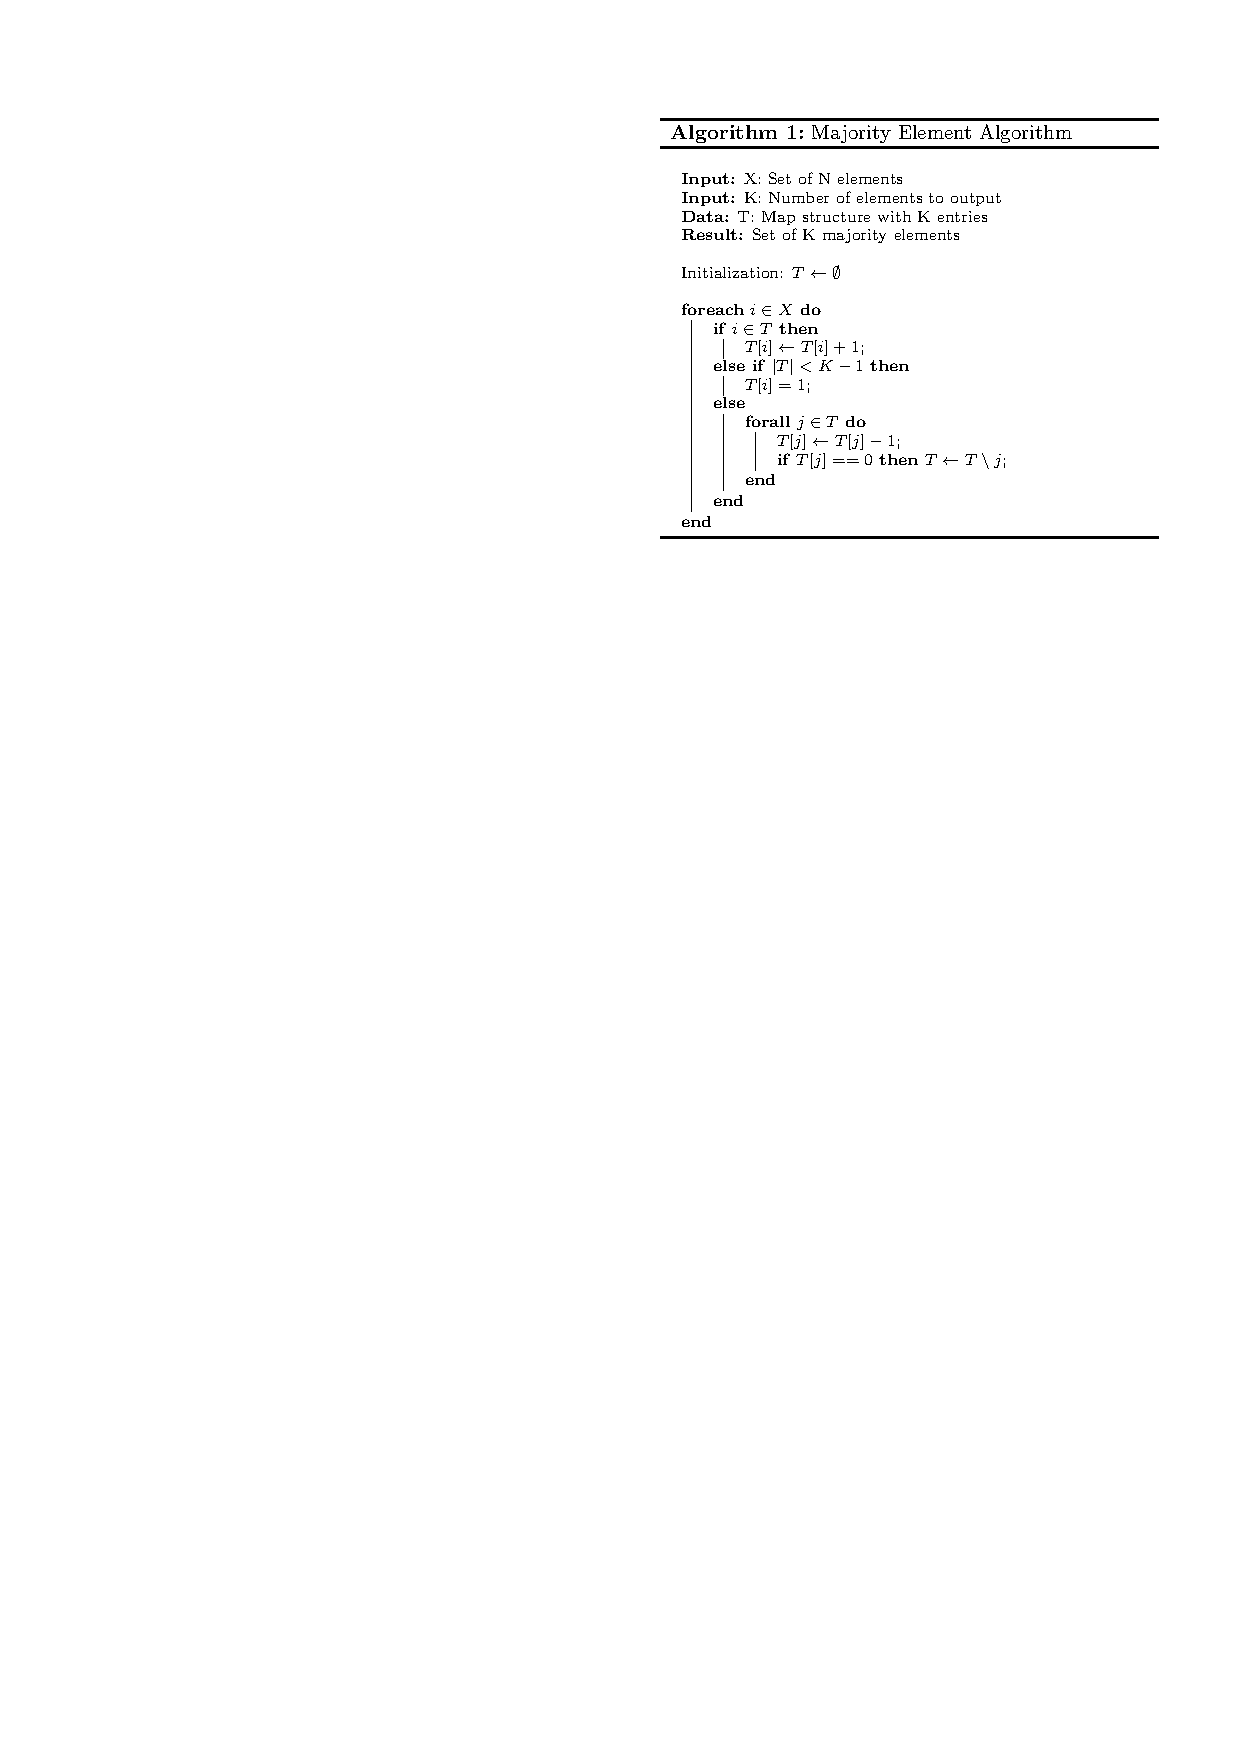
\includegraphics[scale=0.95]{figures/mea_algorithm.pdf}
  
%%%%%%%%% DEAN if you are having issues compiling this on Linux, comment out the algorithm and use the image instead.  
  
  
\end{algorithm}

%\begin{algorithm}
%	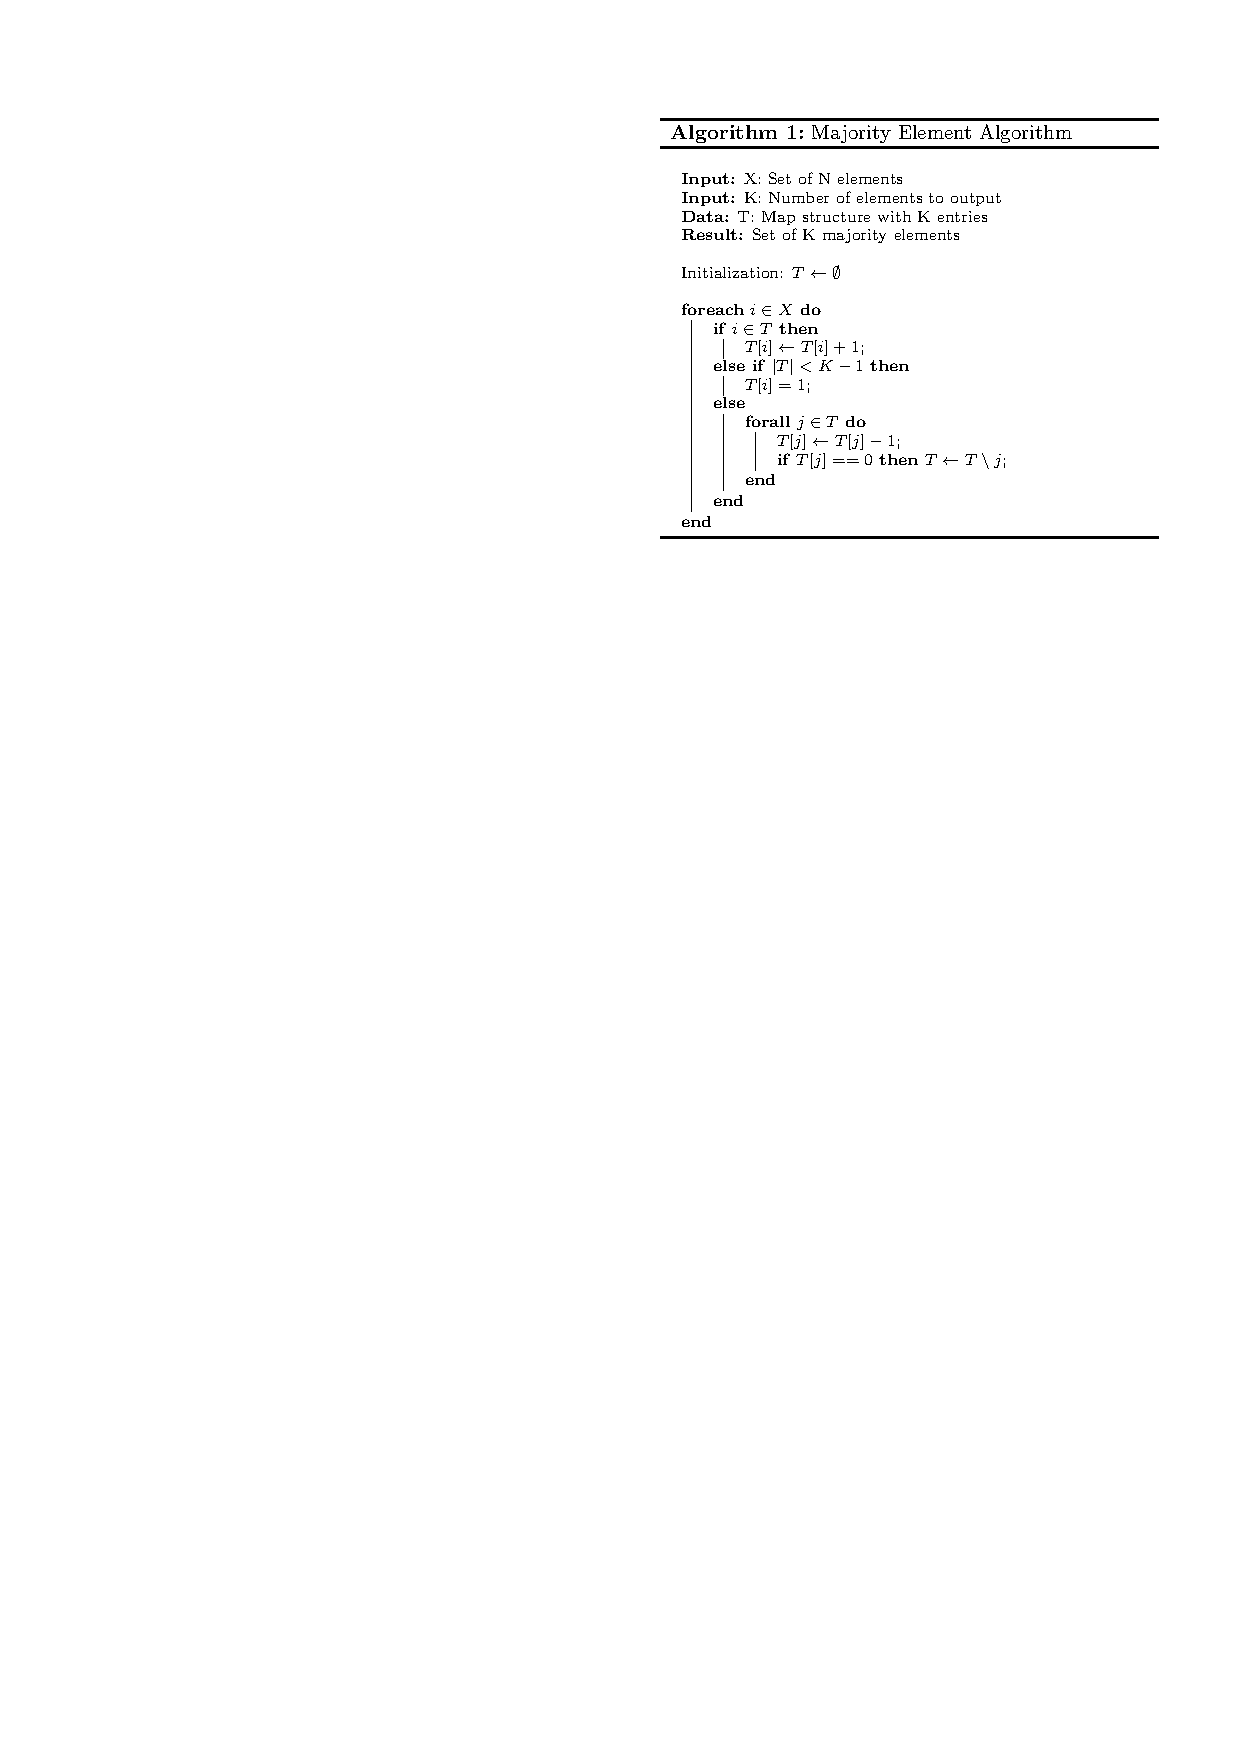
\includegraphics[width=0.45\textwidth]{figures/mea_algorithm.pdf}
%	\caption{TEST}
%	\label{alg:mea}
%\end{algorithm}

MEA is presented in Algorithm \ref{alg:mea} as applied to an array of integers X. A map structure T maps K element IDs (in our integer array example, IDs are the integers' values) to K counters. Looping through the array, if the next integer exists in the map, its counter is incremented by 1. Otherwise, if there's enough room in the map a new entry is added with a count of 1. If the number does not exist in the map and all K counters are occupied, MEA subtracts 1 from every counter, removes the entries with a counter value of 0 and proceeds to the next integer. Once the entire array is processed, the map entries hold the majority elements. 

%Even though this heuristic is 100\% accurate, in the absence of its main assumption no guarantees can be made. The outcome of this algorithm relies on several uncontrolled variables, such as the order our requests appeared in. However, the nature of the algorithm presents a very welcomed side effect: Elements accessed repeatedly can be evicted from the map by elements that were accessed less times but more recently. This observation reveals MEA's favoritism towards temporal locality. Furthermore, the area overhead of this algorithm implemented in hardware remains constant, regardless of how many elements need to be profiled (i.e. regardless of how many pages exist in main memory). 

In our application of MEA to activity tracking, the sequence of page addresses accessed correspond to the array of integers in the above example. 
However, we find that the sequence of accessed pages typically does not
meet the condition of MEA that guarantees it will find the most-accessed
pages; thus, it becomes an approximation.  What makes MEA most useful,
though, is its failure mode -- when it fails to find the most-accessed pages,
it does so by favoring recency over quantity.  That is, a page accessed several
times near the end of an interval can easily knock out a page accessed many
more times early in the interval.  As a result, it combines both access
counting and temporal locality, at a fraction of the cost of access counting
alone.

\remark{Nuwan's comment on next sentence: The "number of regions in memory" isn't really the input set, right? Input set is explained above as the sequence of accesses. Further, it's not entirely true that area overhead is constant with the number of regions. As the region count grows, the size of the map needed to hold those region IDs will grow. Admittedly, it grows as log2(number of regions). So it's very slow growth, but not constant. I won't edit; I'll let you address these points however you see fit.}
\remark{A.P.: I agree that the term input set is wrong here. I updated the text. But I disagree that MEA overhead grows. We could keep it at 128 if we want regardless of the memory size. It's possible that we'll want to use more counters, but the option of keeping it constant is still there}

MEA's area overhead grows slowly with the amount of memory per pod.  The 
number of counters can be kept constant, but the size of the 
ID or tag grows with the log of the memory size.
Its $O(N)$ time 
complexity works well for analyzing a stream of access requests in real time, and eliminates the need for sorting the counters.

%In a memory management scheme that uses Full Counters and a scenario where we want to identify the 100 ``hottest'' pages, we would need one full counter per memory page and on top of that we would have to periodically sort all those counters to pick the top 100. With the use of MEA counters we only need a map with 100 entries regardless of the actual number of pages in main memory. In an 8GB memory with 2kB pages and looking for the top 100 pages, MEA needs $\sim$5K times fewer bits than the full counters' storage requirements (4MB Vs 850B). Considering all the potential benefits MEA can offer in theory, we compared its counting and prediction accuracy against the Full Counters (FC) scheme. 

\subsubsection*{MEA Evaluation}

In this section, we seek to understand the effectiveness of MEA's counting 
and prediction accuracy, compared against a Full Counters (FC) scheme,
independent of the MemPod architecture. We use memory traces captured 
from multi-programmed 8-core workloads (the same traces used and described in Section \ref{sec:Results}) and simulated MEA and FC side-by-side with an in-house off-line simulator that provides oracle knowledge of future intervals. 
\remark{Nuwan's comment on next sentence: What's the significance of 50us here?\\A.P.: At the time, 50us used to be the best interval length for MemPod so I went with it.}

The interval size for both MEA and FC was set at 5500 requests which is the average number of requests serviced within a 50us window in our timing experiments. For this experiment we used 128 MEA counters and FC requires 4.5M counters (assuming a 1+8GB memory capacity). 
We do two comparisons in this study.  First, we examine the ability of MEA
to identify the top pages in the past interval, something the full counter
scheme will do perfectly.  Second, we examine the ability of both schemes
to predict the top pages in the next interval.  In both studies, we will
examine the schemes' ability to identify the 30 most-accessed pages, in
bins of 10 each (1-10, 11-20, and 21-30).

\remark{These results don't make sense without knowing how many MEA
counters you used.\\A.P.: Added in text above.}

Figure \ref{fig:mea_1} shows the counting accuracy of MEA for the 
past interval, which should be compared with FC's perfect accuracy.
In some workloads, MEA identified up to 75\% of the top pages. 
However, on average MEA reports accuracy below 55\% on the top tiers. 
Thus, it is a surprisingly ineffective replacement for accurate counters,
if accurate counting were our priority.  The bias toward recent accesses
has a strong effect on the final value of the MEA counters.

\remark{I find this figure odd -- I'd rather see the results grouped by
benchmark grouping than by tier.\\A.P.: Fixed.}

\begin{figure}[t]
\centering
%  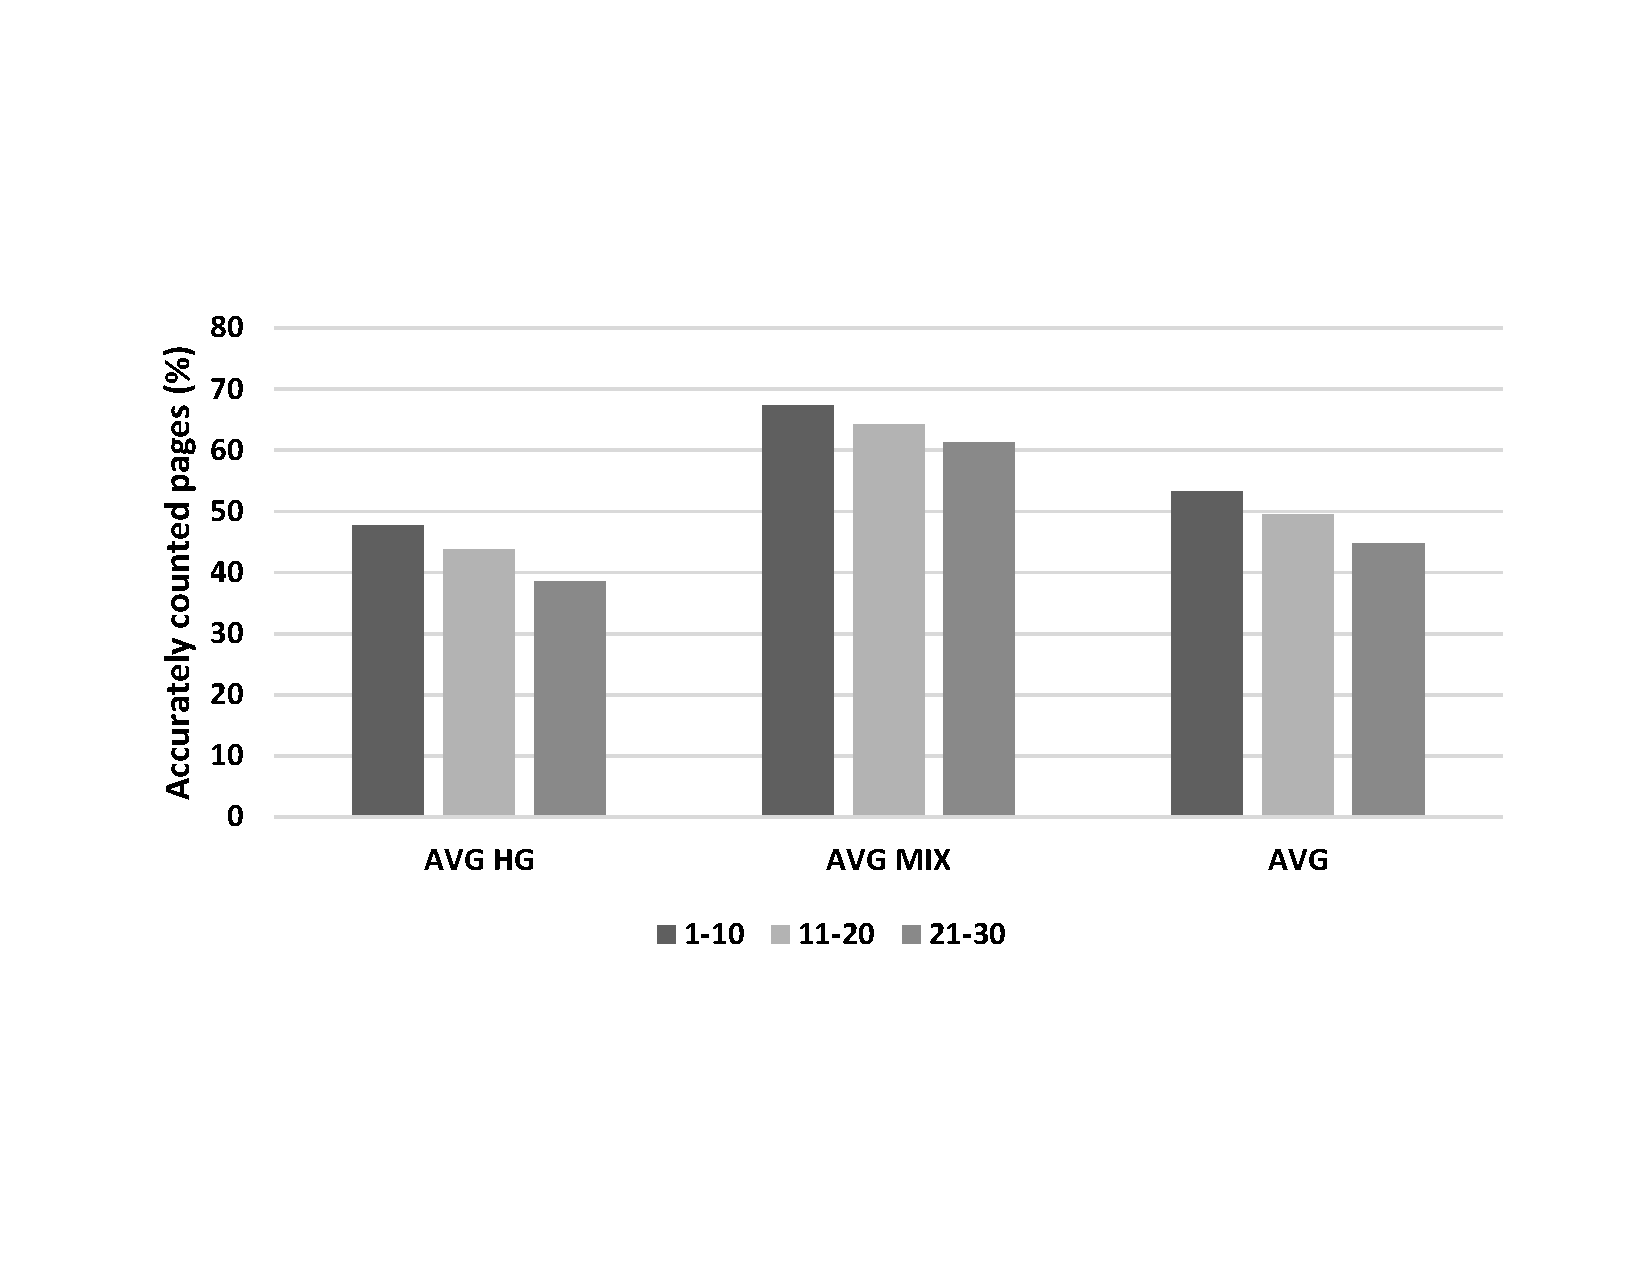
\includegraphics[width=0.46\textwidth, height=9em]{figures/mea_1_v2.pdf}
  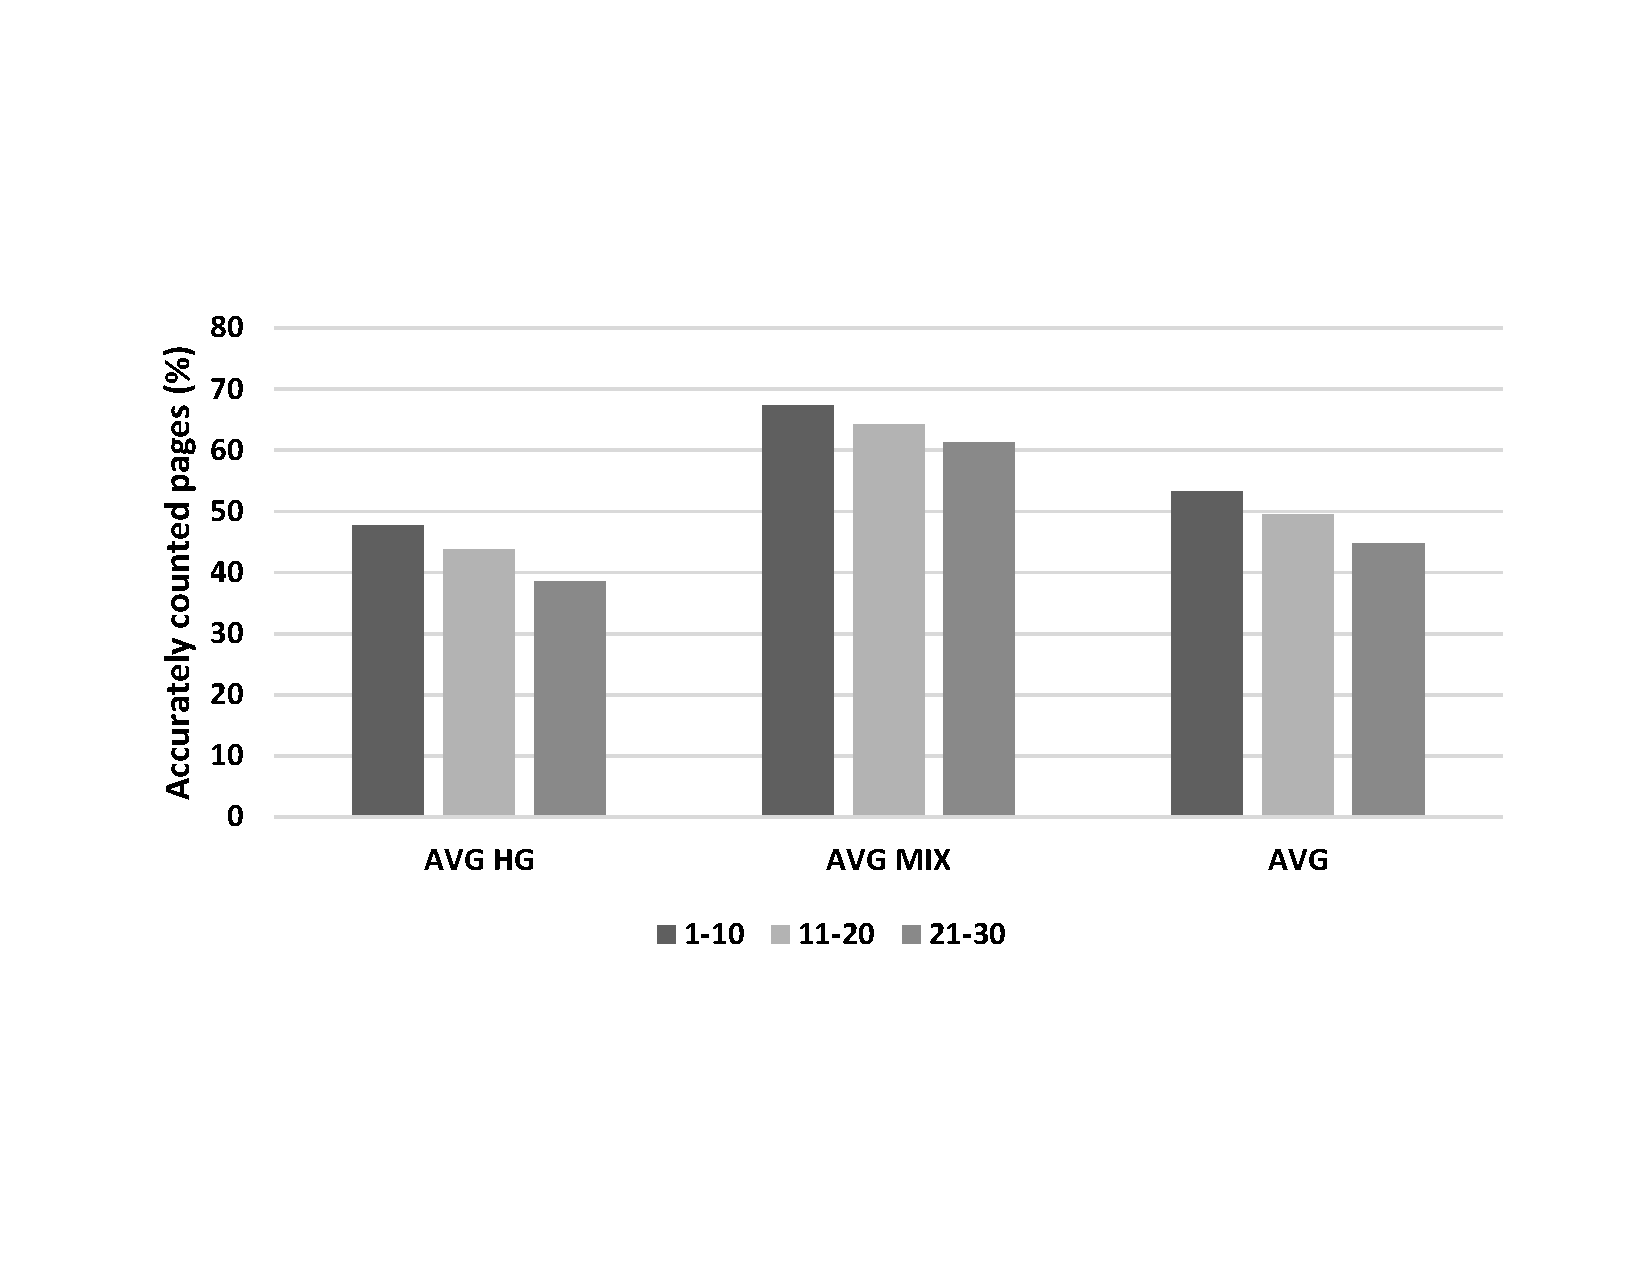
\includegraphics[scale=.3]{figures/mea_1_v2.pdf}
  \caption{MEA counting accuracy compared to Full Counters on the top three tiers (ranks 1-10, 11-20, 21-30). Average results for homogeneous(AVG HG), mixed (AVG MIX) and all (AVG ALL) workloads shown.}
  \label{fig:mea_1}
\end{figure}

When we instead examine the effectiveness in identifying future hot pages,
we see a different story.  Figure \ref{fig:mea_2} presents a comparison of MEA and FC in terms of prediction accuracy. We compare each mechanism's 
``predictions'' against the top three page tiers of the following interval based on oracular knowledge. 
Using 128 counters, MEA will return \textit{up to} 128 predictions based on the past interval, while FC will return an overall ranking of each page accessed. 
In order to be able to directly compare accuracy, 
we take the top N pages from the full counters
each interval,
where N is the number of pages MEA returned.

Figure \ref{fig:mea_2} plots the number of hits on predicted hot pages from the previous interval. We also selected interesting individual benchmarks and show them in Figure \ref{fig:mea_3} to provide a more detailed comparison. 

\remark{Here we're again missing all the critical
details of the experiment.  How many
MEA counters?  How many FC pages were used as ``predictions''?\\A.P.: 128 MEA counters. I used the number of pages MEA returned at each interval as the number of predictions for both mechanisms. Added in text above.}

On average, MEA achieves more future hits than FC by 16\%, 81\% and 68\% on the top three tiers respectively. Figure \ref{fig:mea_3} shows selected individual workloads that generated interesting results and provides a more detailed comparison. Cactus\footnote{We use a single benchmark's name as a shorthand for workloads running the same benchmark 8 times simultaneously on 8 cores.} is the only workload where FC outperformed MEA's prediction. In fact it outperformed MEA on every tier. 

Xalanc and mix9 are most representative of our overall
results. We can see MEA outperforming FC's prediction accuracy in every bin. 
The last two workloads we selected, bwaves and lbm, show FC failing entirely to predict the future (FC also scored zero future hits with our libquantum workload). With bwaves (and libquantum) MEA reports a very low number of future hits but not zero. These results can happen when an application streams through large structures
that exceed the size of the interval.  In that case, the past interval has 
little overlap with the next interval, but recent accesses are much more
likely to be overlapped.
Lbm shows an interesting result, where MEA reports 
a high number of hits (outside of the first tier) in a workload where 
FC failed entirely.  This can happen with a large working set where the 
application does a fairly constant amount of work per page.  Full counters,
then, will record the highest access counts for pages the application is done
with, while MEA will favor pages the application was still working on at the
end of the interval.

\begin{figure}[t]
\centering
  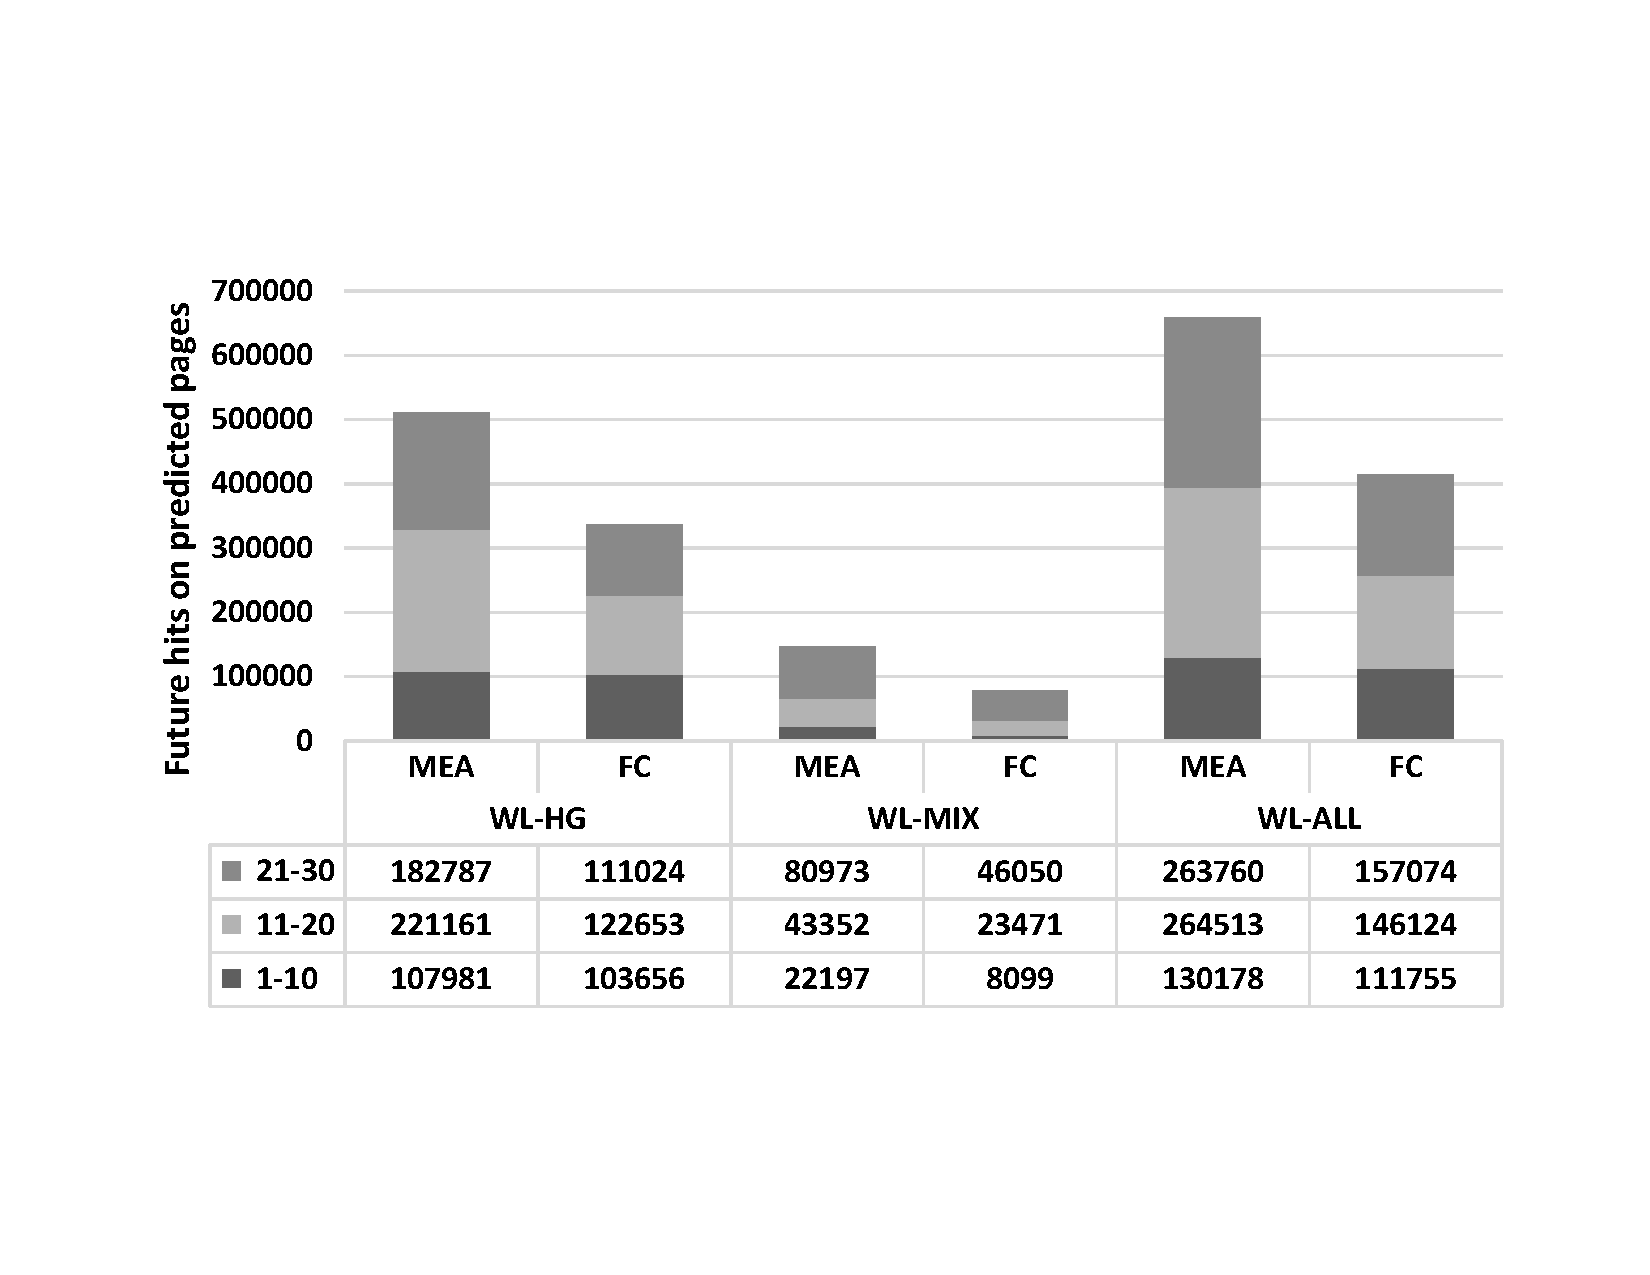
\includegraphics[scale=.3]{figures/mea_2_v2.pdf}
  \caption{MEA prediction accuracy (part 1) compared to Full Counters on the top three tiers (ranks 1-10, 11-20, 21-30). Results for homogeneous(WL-HG), mixed (WL-MIX) and all (WL-ALL) workloads shown.}
  \label{fig:mea_2}
\end{figure}

\begin{figure}[t]
\centering
  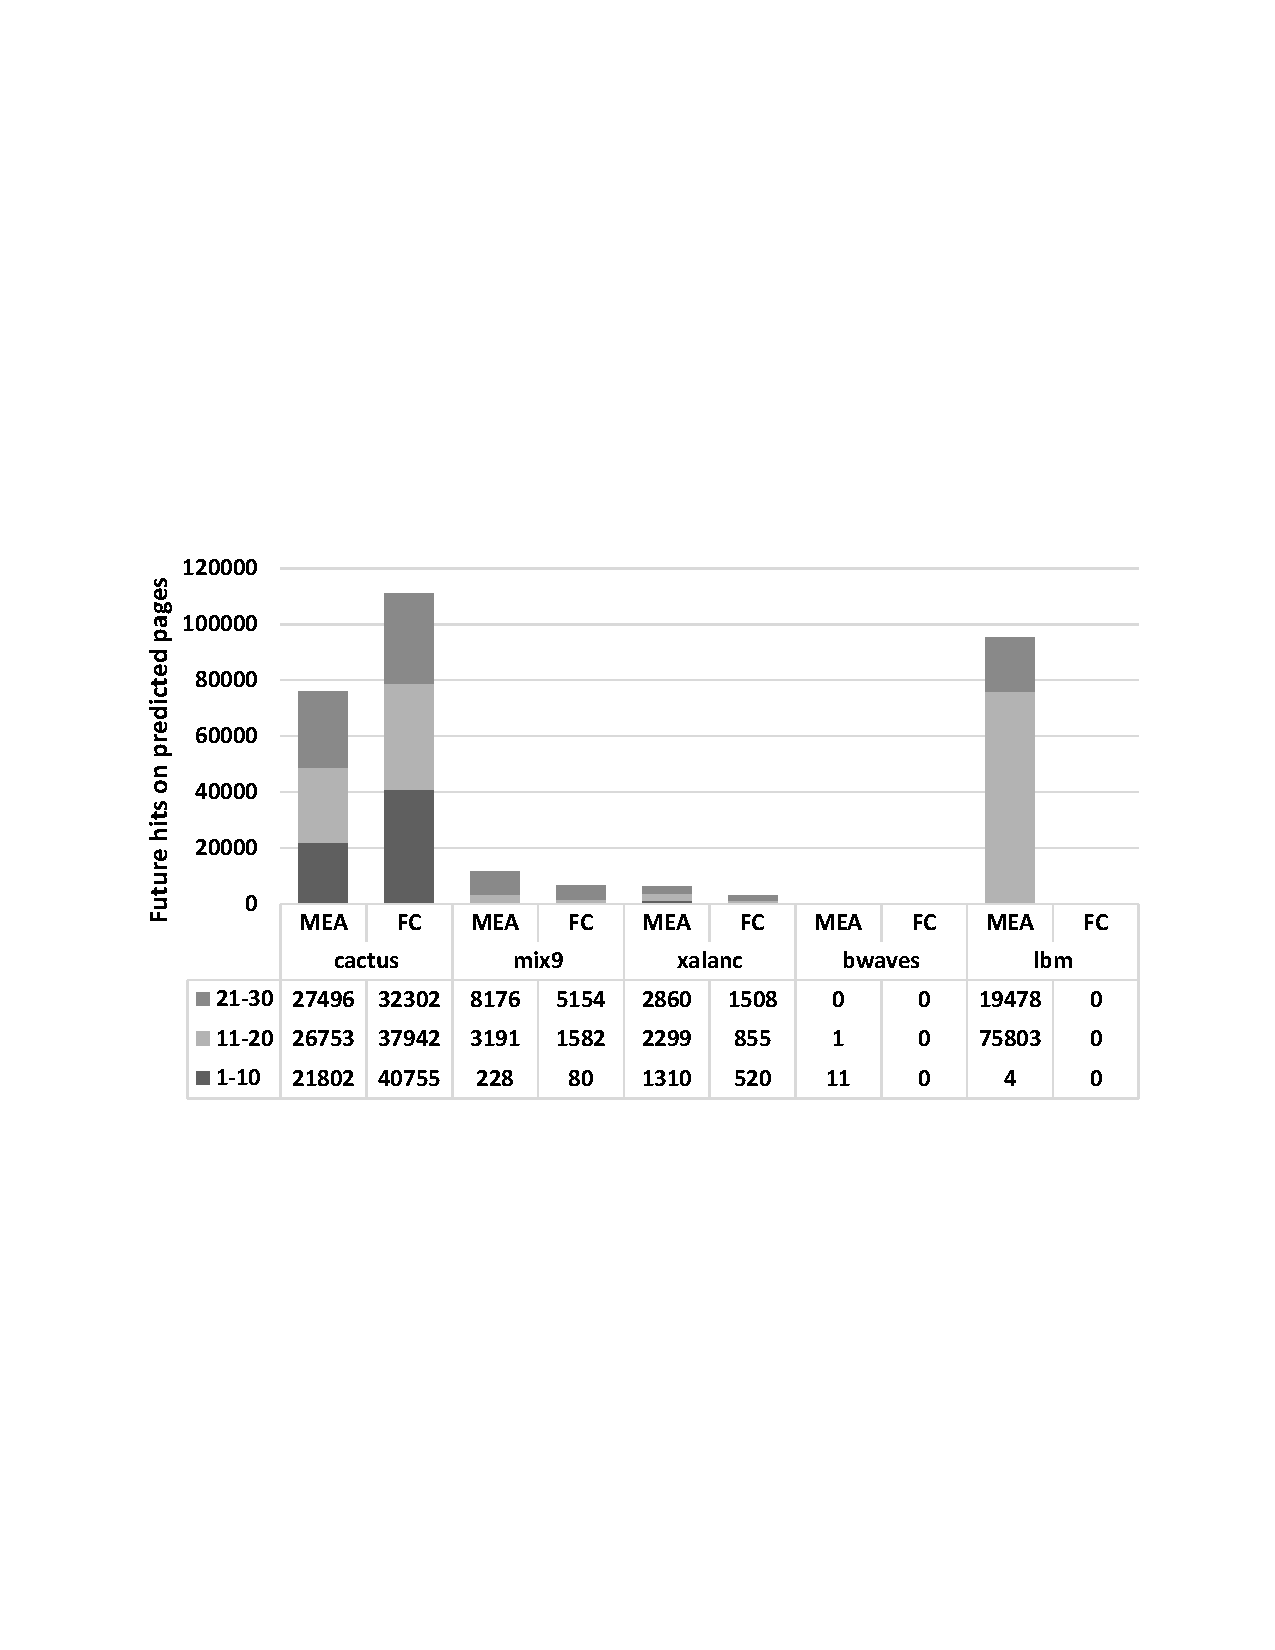
\includegraphics[scale=.45]{figures/mea_3_v2.pdf}
  \caption{MEA prediction accuracy (part 2). This graph presents the most interesting results from individual workloads.}
  \label{fig:mea_3}
\end{figure}

MEA has not previously been used in any kind of architectural event
tracking; however, our results indicate it is an attractive
alternative to full counters at a very small fraction of the hardware cost.

% !TEX root = ../MemPod.tex
\section{Architecture}
\label{sec:Architecture}

Our clustered migration mechanism is designed to address key challenges associated with the migration problem. In this section, we present a complete description of our micro-architectural design, followed by a breakdown of the important design decisions, along with the corresponding challenge addressed by each one.

%\begin{table*}[t]
%\begin{tabularx}{\textwidth}{ |X|X|X|X|X| }
%  \hline
%    \textbf{Challenge} & \textbf{Tradeoff} & \textbf{THM} & \textbf{HMA} & \textbf{MemPod} \\ \hline       
%    Page Relocation & Flexibility / Time & Only 1 candidate \newline (Minimum / Very low)& No restrictions \newline (Max / High) & Intra-Pod migration \newline (High / Medium) \\ \hline
%    Remap Table Size & Flexibility / Area & 1 entry per fast page \newline \textasciitilde2.4MB \newline (Minimum / Medium) & No remap table \newline 0 Bytes \newline (Max / Min) & 1 entry per fast page \newline 4.5MB (1.125MB/Pod) \newline (High / Medium) \\ \hline
%    Activity Tracking & Accuracy / Area & 8 bits per fast page \newline 64kB \newline (Medium / Low) & 16 bits per page \newline 1.125MB \newline (Max / Max) & 48 bits per fast page \newline 384kB \newline (High / Medium)\\ \hline
%    Migration Trigger & N/A & Threshold based & Interval based & Interval based\\ \hline
%    Tracking Organization & Simplicity / Parallelization & Fully Centralized \newline Serialized requests \newline (High / Min) & Fully distributed \newline (High / Max) & Semi-distributed \newline Pods operate independently \newline (High / High)\\ \hline
%    Migration Driver & Communication cost & CPU \newline High latency \newline (Max) & CPU (OS) \newline High latency \newline (Max) & Pod \newline Very low latency \newline (Low)\\ \hline
%    Migration Cost & Time & HW cost + communication \newline (Medium) & HW + SW + cold TLBs \newline (Max) & HW cost \newline (Min)\\ \hline
%\end{tabularx}
%  \caption{Breakdown of state-of-the-art designs}
%  \label{tab:comparison}
%\end{table*}

\begin{table}
  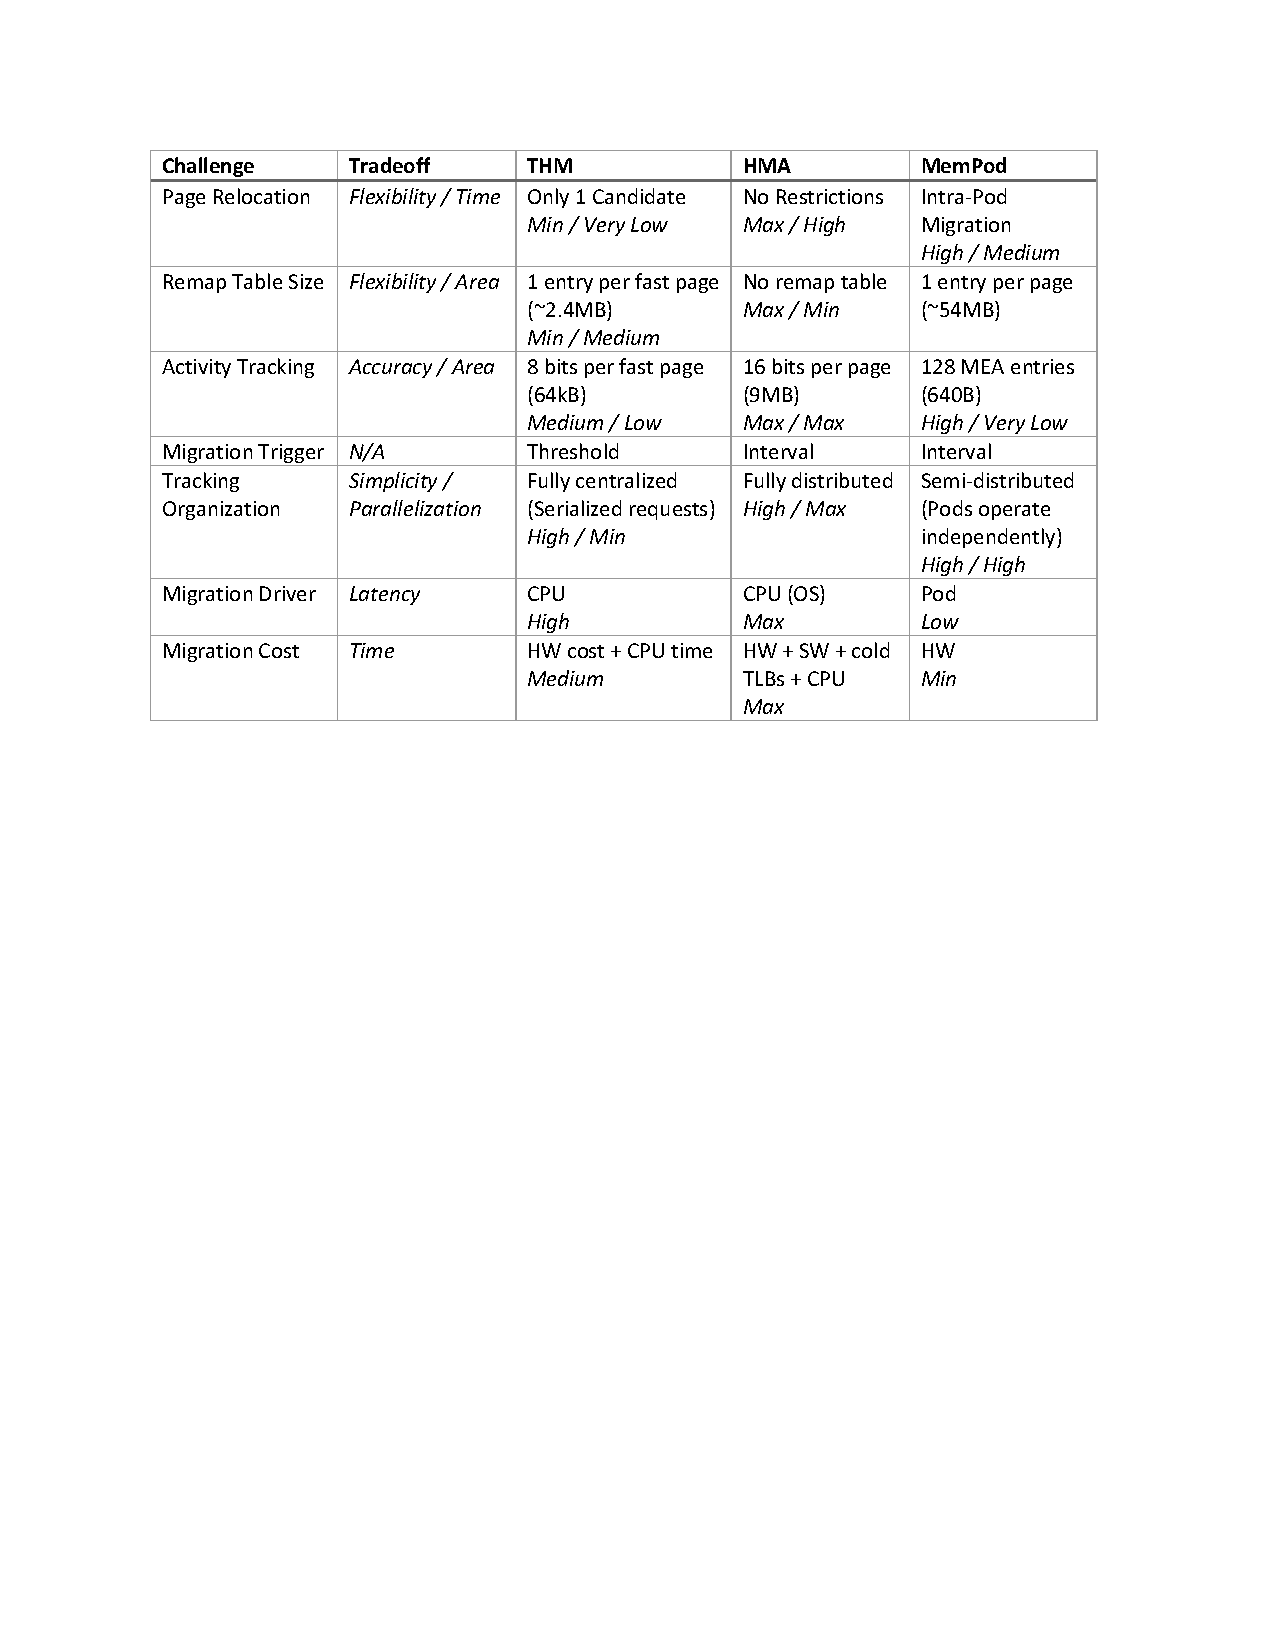
\includegraphics[width=\linewidth]{figures/comparison_table.pdf}
  \caption{Breakdown of state-of-the-art designs}
  \label{tbl:breakdown}
\end{table}

\subsection{Clustered Migration Architecture}

 Figure \ref{fig:architecture_complete} presents an overview of MemPod. MemPod's design was kept modular to facilitate system integration and scalability. A number of memory ``Pods'' are injected between the LLC and the system's memory controllers (MCs). Each Pod clusters a number of MCs and enforces migrations to only occur among its member MCs. Pods do not communicate with each other, preventing inter-Pod migrations. To the rest of the system, Pods are exposed as MCs. With MemPod's transparent design, each Pod will now be receiving all the requests originally addressed to any of the Pod's member MCs. 
 
\begin{figure}
 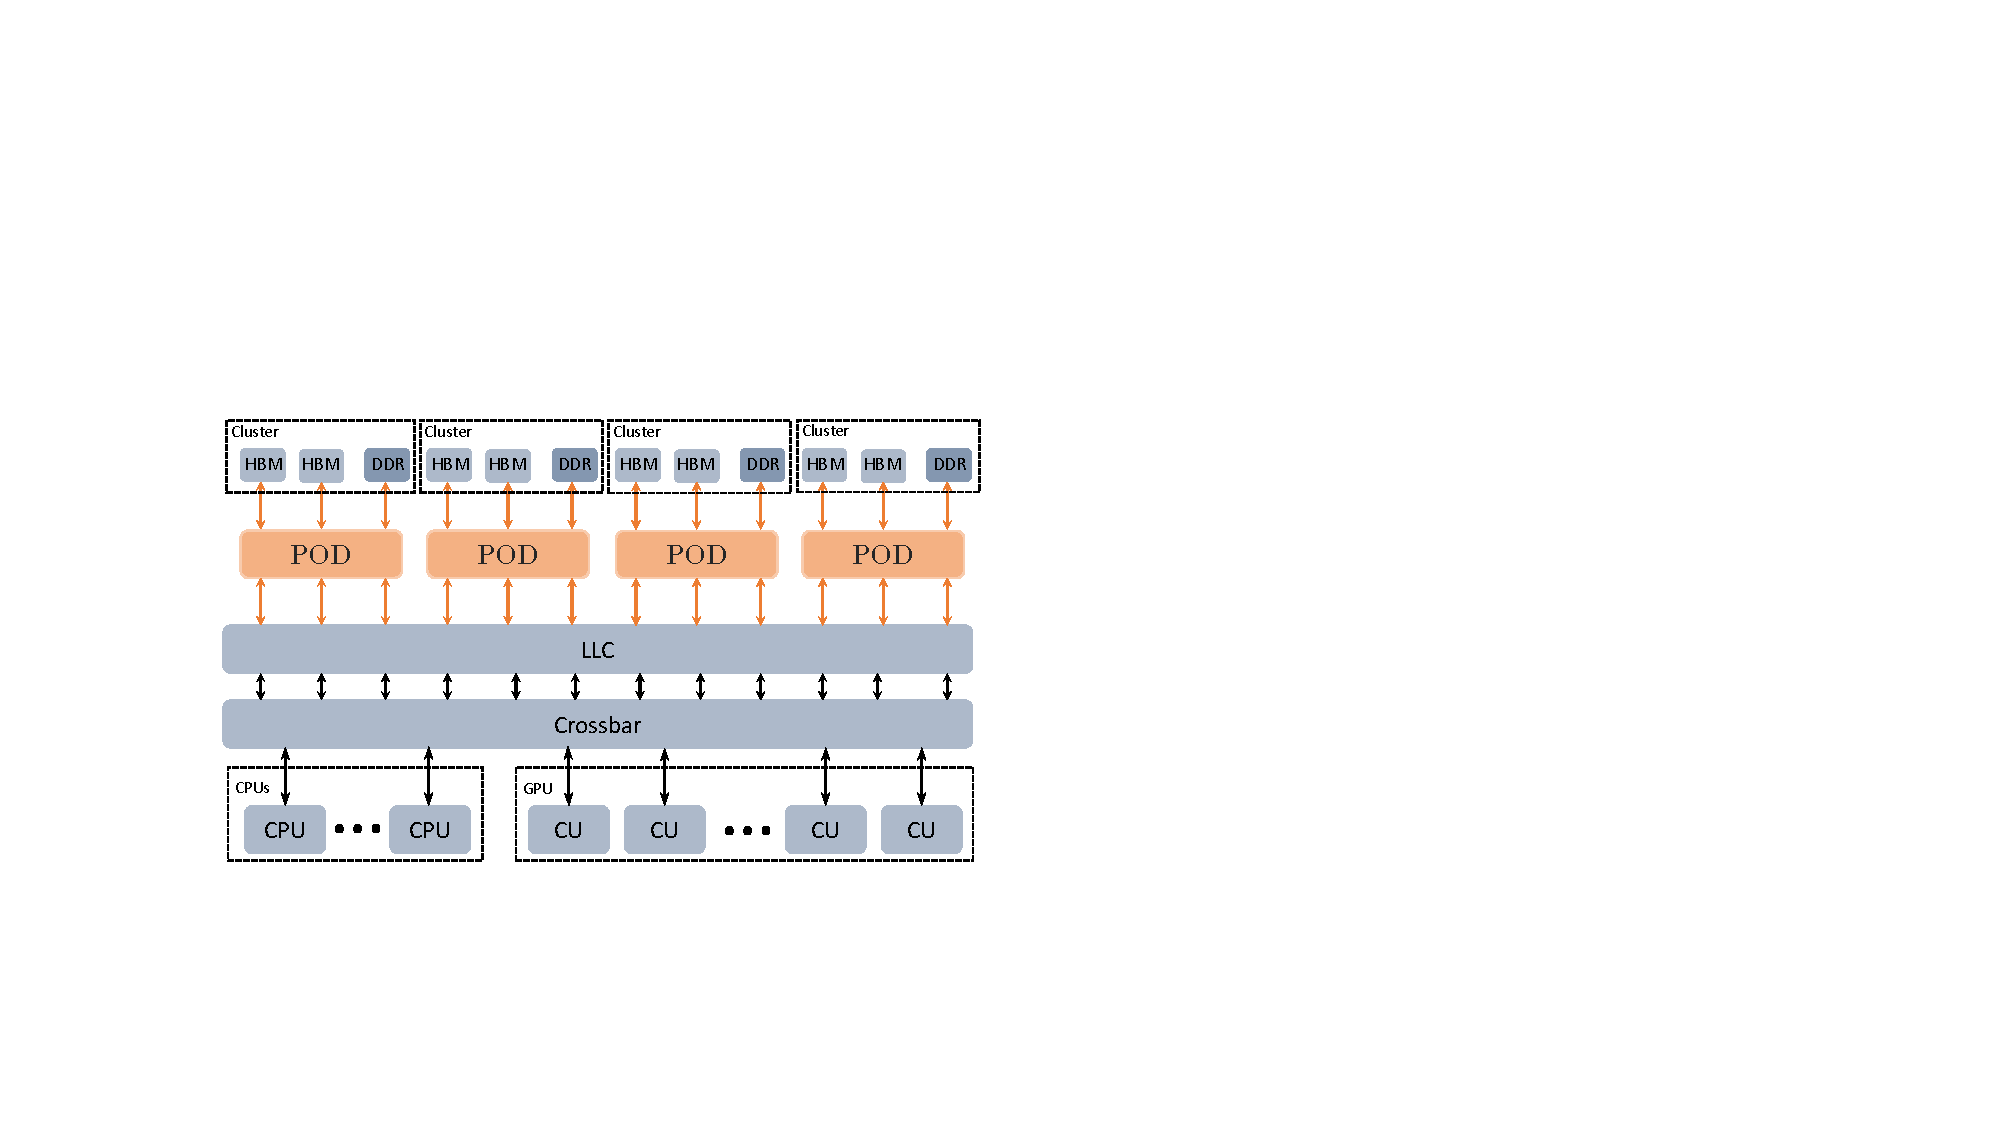
\includegraphics[width=0.47\textwidth]{figures/mempod_org.pdf}
 \caption{MemPod high-level architecture}
 \label{fig:architecture_complete}
\end{figure}

When a memory request arrives, the Pod monitors the request, updates any 
necessary migration-related activity tracking counters, and forwards 
the request to the intended recipient MC. The migration logic within a Pod does not need to be invoked during a response from any MC and can be bypassed to reduce memory access latency. A drawback of clustering MCs into Pods is the serialization of potentially parallel requests to different MCs of a single Pod. As such, activity tracking within a Pod as well as the subsequent forwarding of requests must be as efficient as possible. 

MemPod's clustered architecture also aids in reducing global traffic during migrations compared to non-partitioned mechanisms.  Because migration
traffic happens within a Pod, this architecture significantly reduces global
traffic and enables highly parallel migrations.
%  Higher global traffic could require the global switch (or crossbar) to have higher bandwidth resulting in increased energy costs and could also introduce performance penalties. Furthermore, with Pods servicing migrations transparently, the system's CPUs will be able to keep executing non-memory instructions during migrations. 

\subsubsection*{Memory Pod}

The major architectural elements of a Pod are shown in Figure \ref{fig:architecture_pod}. A Pod includes an activity tracking (MEA) unit, a remap table for keeping track of migrated pages and a forwarding unit that can re-encode a request with the relay address and, based on that address, send the request to the appropriate MC.
%
%\begin{figure}[h]
%  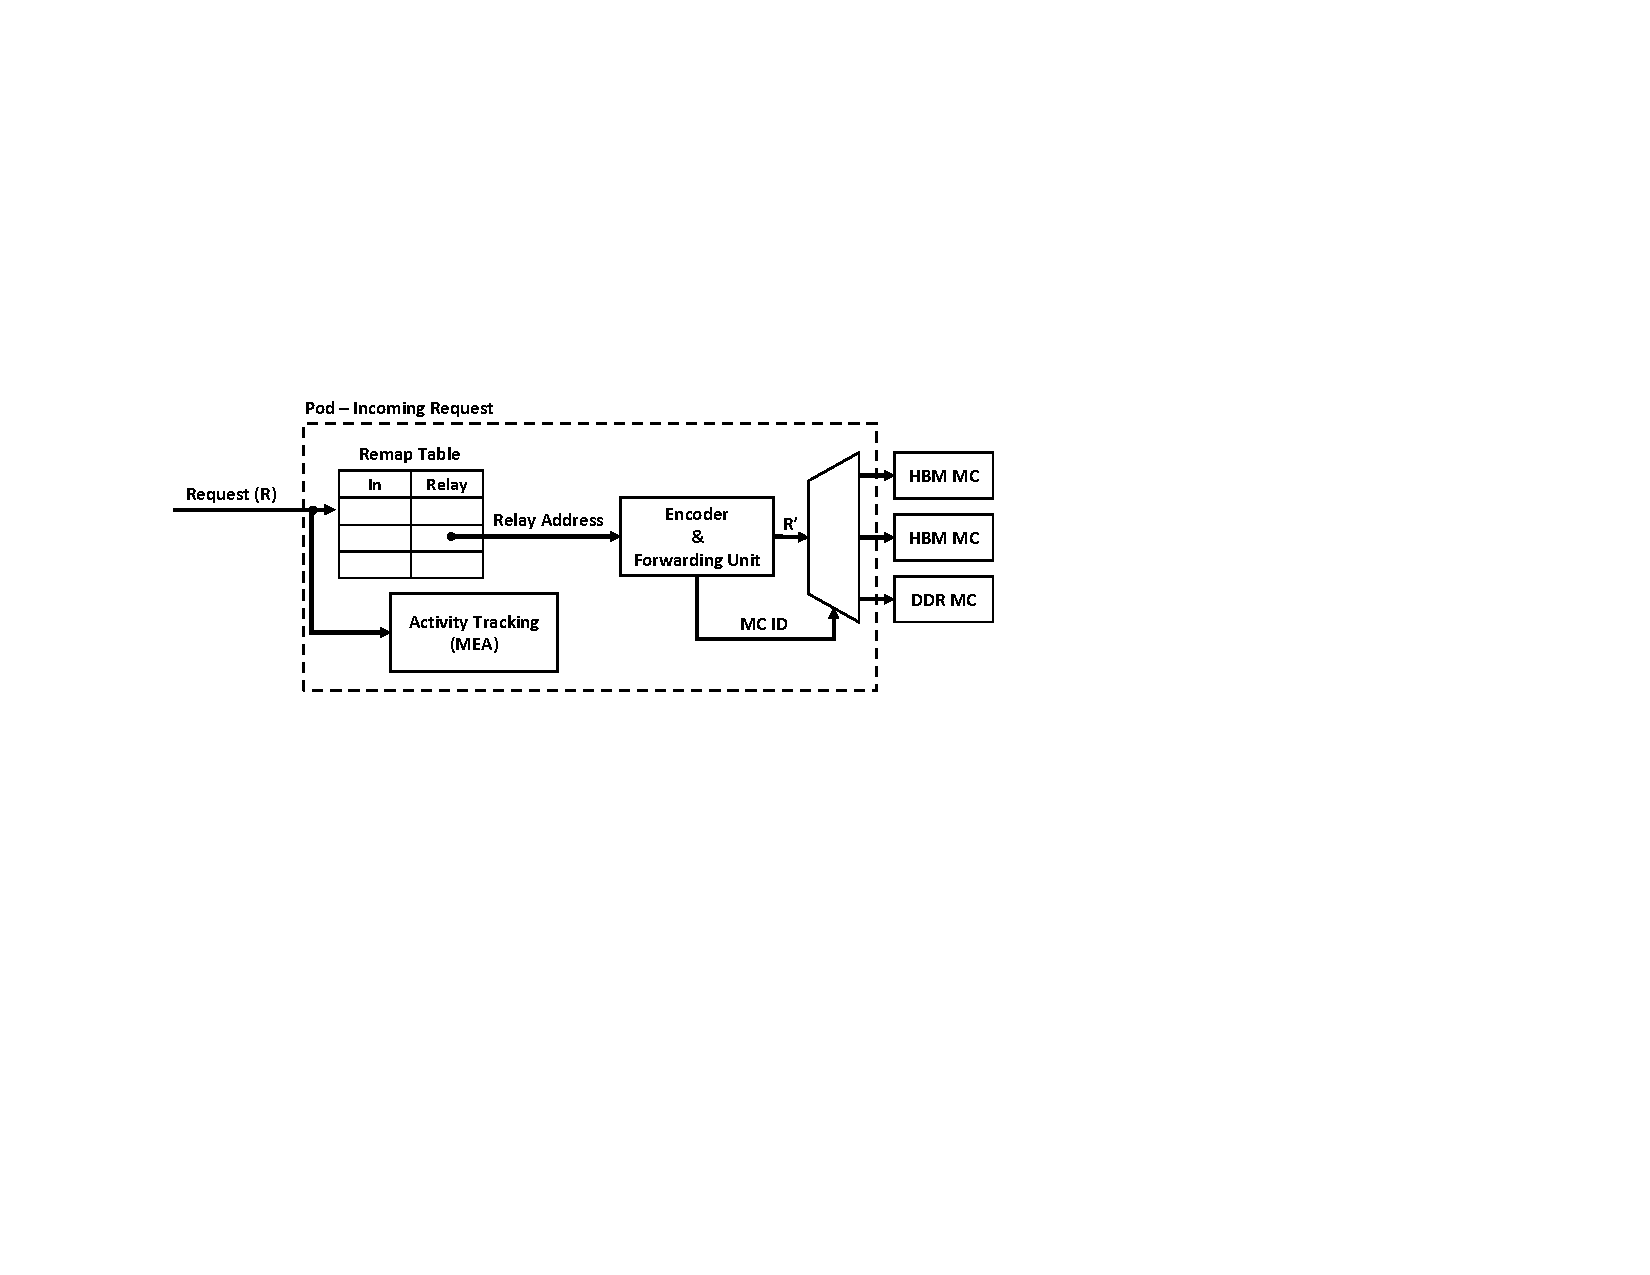
\includegraphics[width=0.46\textwidth]{figures/pod_design_request.pdf}
%  \caption{Major architectural Pod elements}
%  \label{fig:architecture_pod}
%\end{figure}

\begin{figure}
\begin{subfigure}{0.46\textwidth}
  \centering
  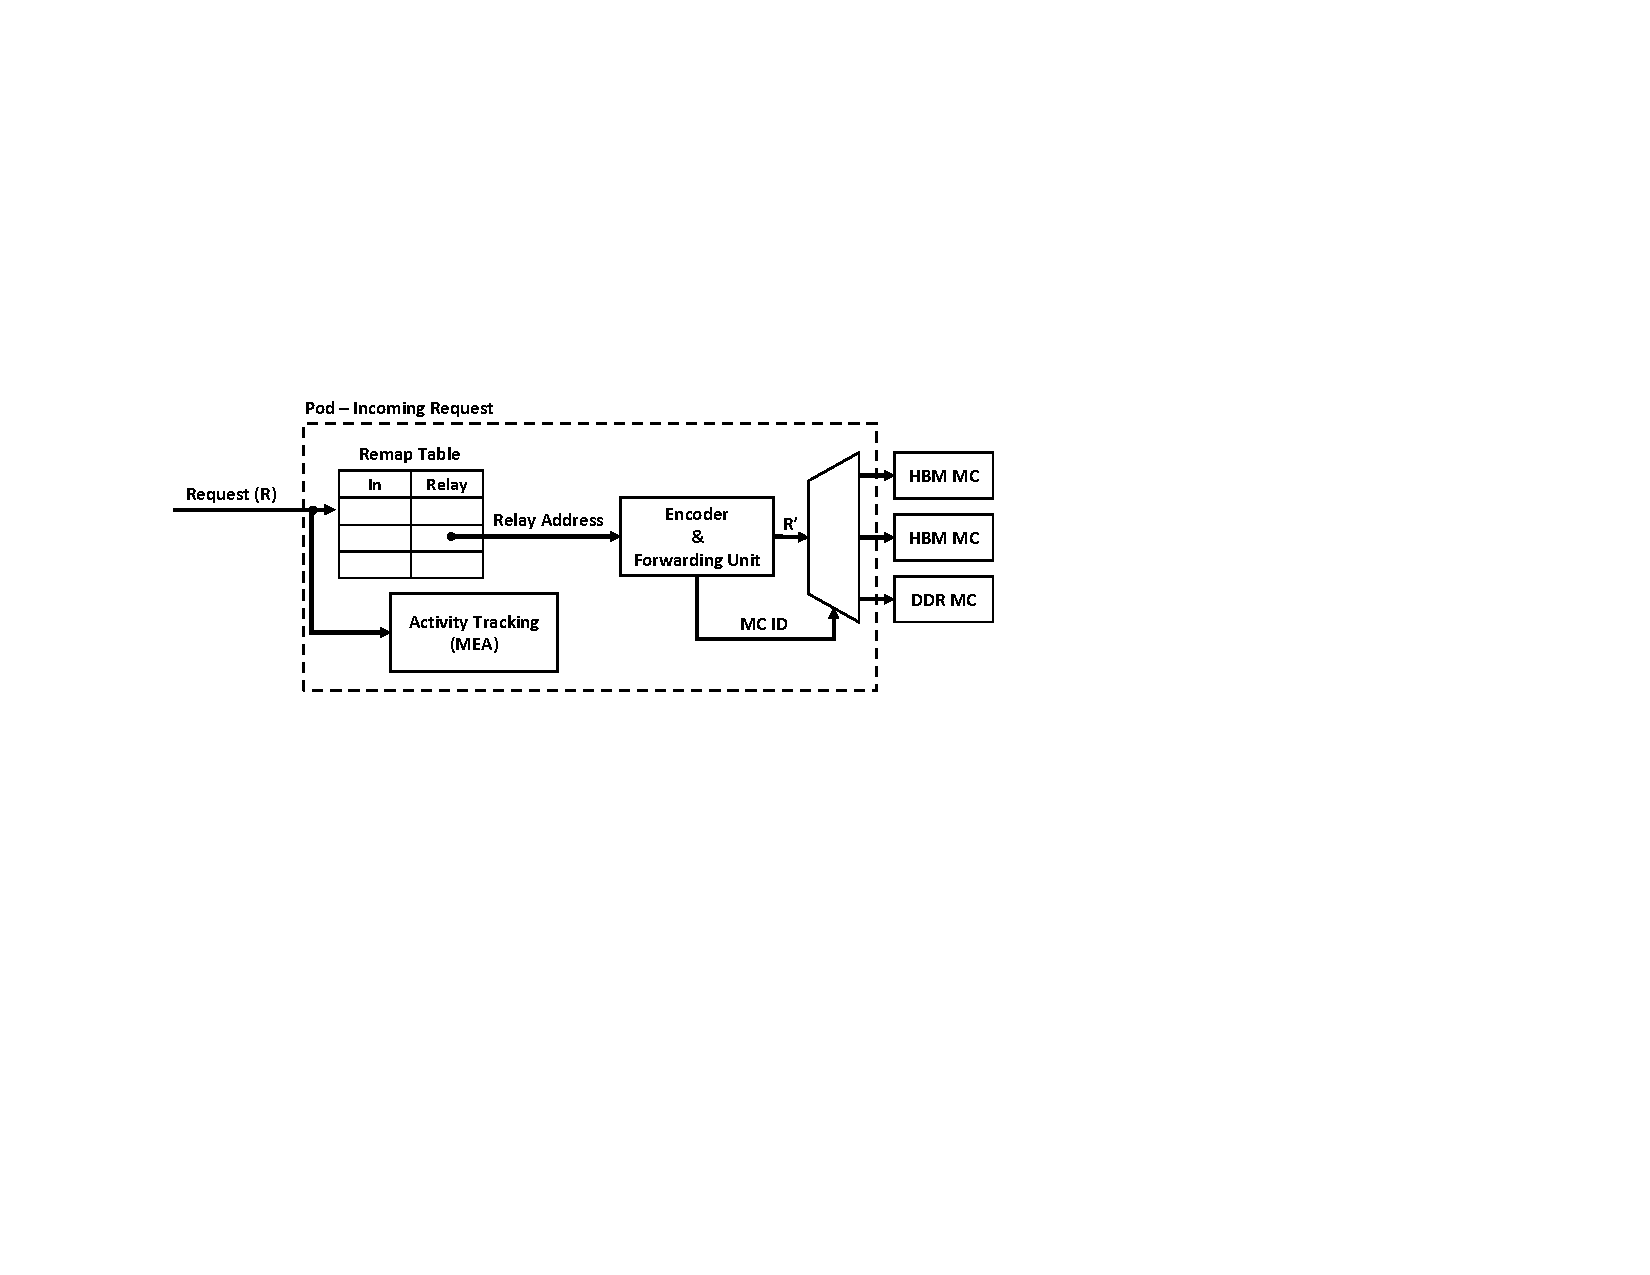
\includegraphics[width=\textwidth]{figures/pod_design_request.pdf}
  \caption{Pod's request forwarding operation}
\end{subfigure}%

\begin{subfigure}{0.46\textwidth}
  \centering
  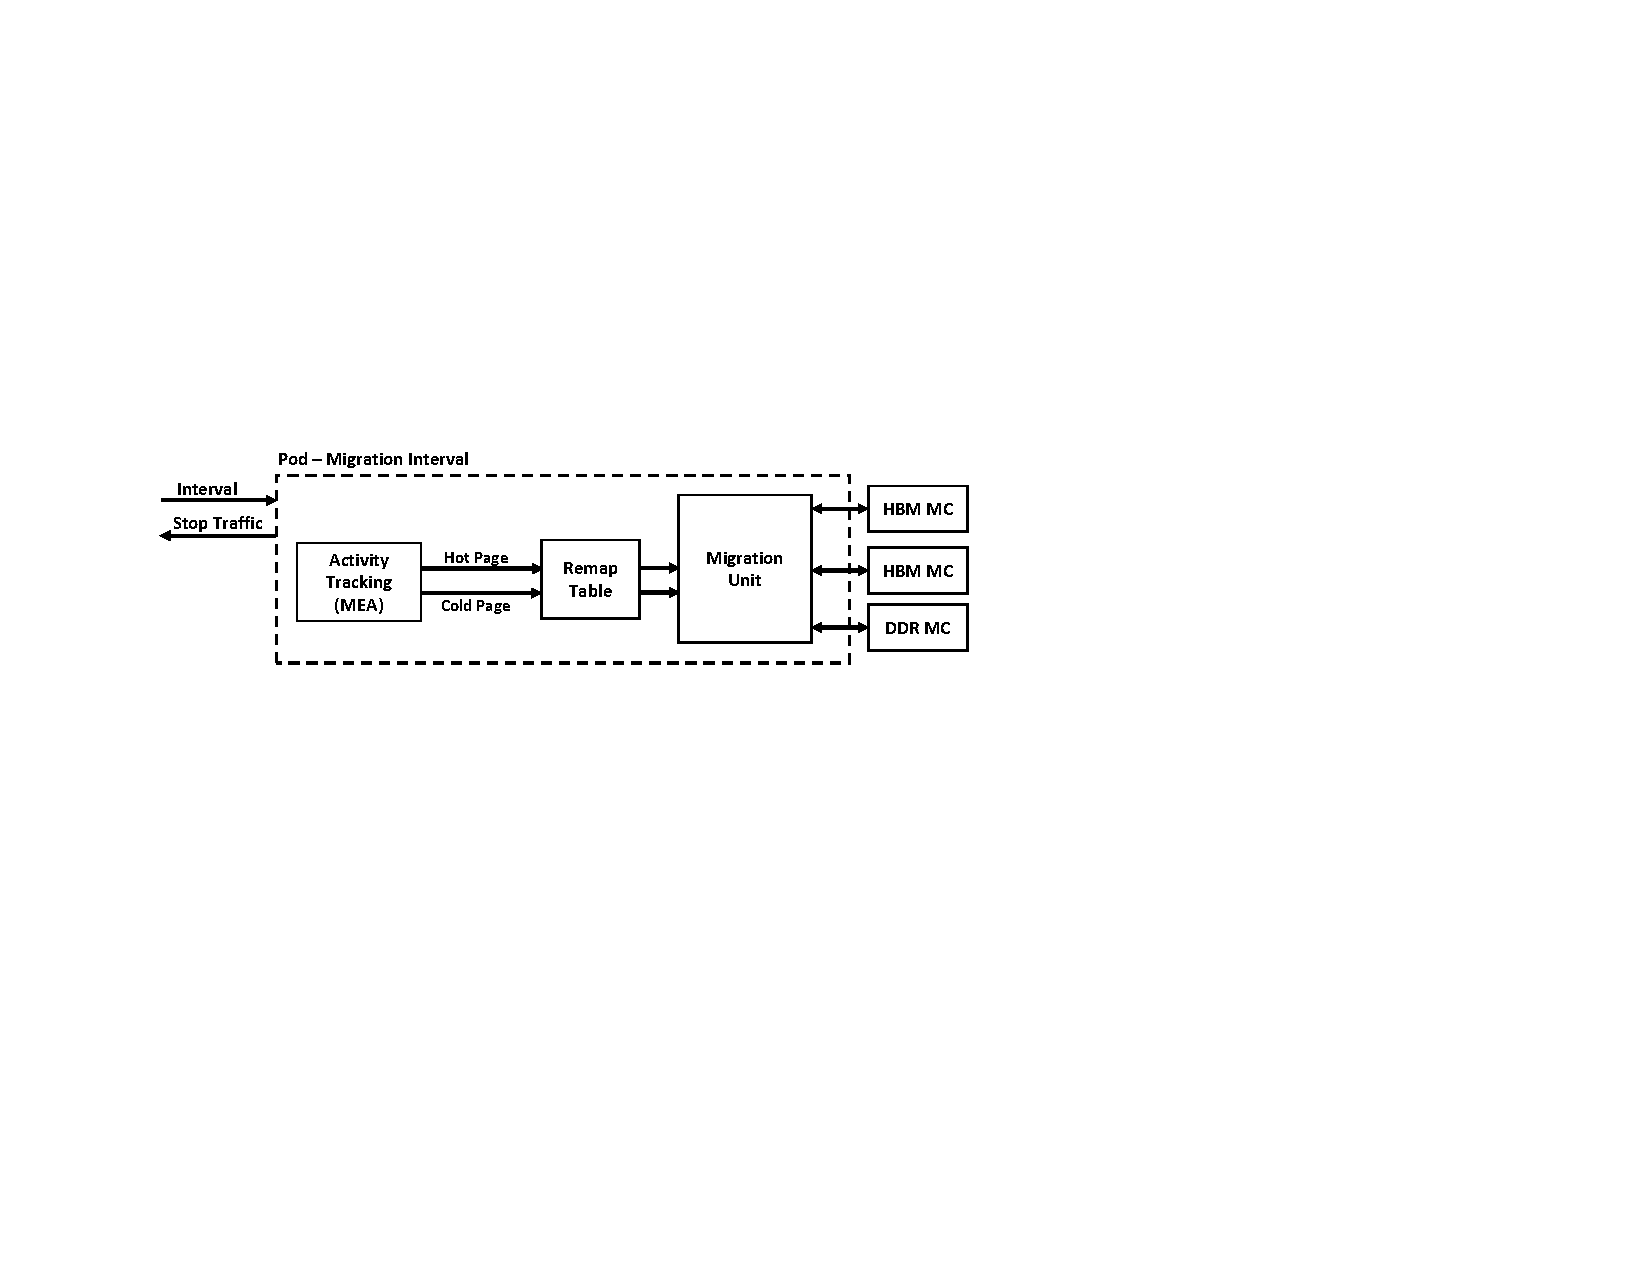
\includegraphics[width=\textwidth]{figures/pod_design_migration.pdf}
  \caption{Pod's migration procedure}
\end{subfigure}
\caption{Major architectural Pod elements}
\label{fig:architecture_pod}
\end{figure}

A designer can vary the parallelism and flexibility of MemPod by varying the
number of Pods. A design with one Pod is equivalent to a centralized 
migration controller allowing any-to-any migration,
%\footnote{Any-to-any migration: page migration without constraints on source and destination. All MCs can migrate a page to any other MC.}, 
while a design with a Pod number equal to the number of MCs would imply that migration is disabled. A reasonable design point would be to set the number of Pods equal to the number of slow-memory MCs. Such a configuration inherently restricts migration between slow off-chip channels, while at the same time maintaining full channel-level parallelism on the system's bottleneck: the slow MCs. In a configuration where the number of fast-memory MCs are not a multiple of slow-memory MCs, Pods can be configured asymmetrically or some MCs could be members of multiple Pods, with their capacity partitioned to avoid crosstalk issues. In Figure \ref{fig:architecture_complete} we present a system with eight MCs for the fast, on-die stacked memory and four MCs for the slow off-chip memory. Throughout this paper we use die-stacked HBM as the fast memory \cite{JEDEC-HBM-REVISED} and DDR4-1600 as our off-chip memory, and
%The use of four Pods imposes few restrictions on migration possibilities, while forbiding migration between two slow-memory channels without any additional logic. 
we set the number of Pods to four, as shown in Figure~\ref{fig:architecture_complete}.

\subsection{Distributed Migration Controllers}

\remark{A.P.: This used to be the Decentralization subsection. Let's see if it works better here. I'm basically rewriting the whole thing. The purpose of this subsection now is to explain the benefits of distributed migration controllers such as Pods compared to centralized units.}

Migration mechanisms in the literature \cite{sim-micro2014,cameo} assume a centralized migration controller which all memory requests have to go through before reaching the memory, in order to monitor memory activity, read remap tables and control migrations. MemPod's distributed migration controllers control every aspect of the migration process. The use of four Pods breaks the problem into smaller pieces in a divide-and-conquer approach. Instead of trying to identify the N best pages to migrate from the entire memory, each Pod now has to identify the $N\over4$ pages per Pod. 
%The hardware breakdown can also simplify the manufacturing process. Smaller tables are more efficient than larger tables and can be designed to meet timing constraints easier. 
Each Pod will also require lower bandwidth than a centralized unit as it handles a fraction of the traffic.

Prior publications \cite{loh-isca08} demonstrate that the layout and address interleaving of main memory and last level cache can be co-designed and benefit a system by increasing efficiency and reducing global traffic. The proposed designs align cache ``banks'' with main memory banks (among other optimizations). Even though not specifically proposed for 3D DRAM memories, if such a design is assumed, a centralized migration controller would be detrimental to the carefully designed alignment since all LLC misses will now have to go through the centralized unit and then fan back out to their respective MCs.

Finally, a clustered design ensures that we are never moving data across the entire system. Migration can only occur within a Pod and between ``sibling'' MCs. By limiting migration distance, MemPod imposes a tighter ceiling on data movement energy which can lead to migration-related energy savings when compared to a centralized design.


\subsection{Building Blocks}

The design of a complete memory manager can be broken down into the following 5 ``building blocks'':
\begin{description}[style=unboxed,leftmargin=0cm]
\setlength\itemsep{0em}
\item [Migration flexibility:] Defines which areas in memory can be used as migration candidates. 
%Higher flexibility offers more potential for performance improvement and increases book-keeping cost.
\item [Remap table:] A structure that keeps track of migrated pages and is able to provide a relay address given a requested address.
\item [Activity tracking:] Logic and structures needed to profile memory requests and predict future ``hot'' pages.
\item [Migration trigger:] Defines when migration occurs. Usually the trigger can be interval-based or threshold-based.
\item [Migration driver/datapath:] Defines the path followed and the hardware modules involved in performing migrations.
\end{description}

Each of the above building blocks introduces some trade-off. For example, allowing more flexibility in migration locations can lead to higher performance benefits, at the cost of larger book-keeping structures. Table \ref{tbl:breakdown} shows a comparison of each mechanism's elements. The following subsections provide a detailed description of each building block. For each block, we present MemPod's, THM's and HMA's approach.
The design choices for the various building blocks are largely
orthogonal.  Thus, we describe each separately, with description of the options
and tradeoffs.

\subsubsection{Migration Flexibility and Remap Table Size}
\label{sec:relocation}

Migrating pages can provide the highest benefit when no restrictions are imposed on the available migration locations.  This amount of flexibility, however,
requires more bookkeeping and can incur a higher cost.

A hardware-driven migration mechanism requires some kind of remap table,
commonly implemented as a hash structure, indexed by a page's address and pointing to the migrated (or relay) page address if one exists. On a page migration, the remap table is updated to reflect the new address of a migrated page. 

The remap table should provide the remap, or relay, address for each original
page address.  Some other structures may also be necessary to avoid expensive
table searches when an inverse lookup is needed (e.g., to identify pages
currently mapped to slow or fast memory).

\ignore{
However, a ``naive'' remap table design can fail when re-migration of pages is allowed. A content-aware remap table is necessary in order to support re-migration. Figure \ref{fig:remap_table_comparison} presents a side-by-side comparison of the operation of these two tables and demonstrates how a naive table can fail.

\begin{figure}[h]
  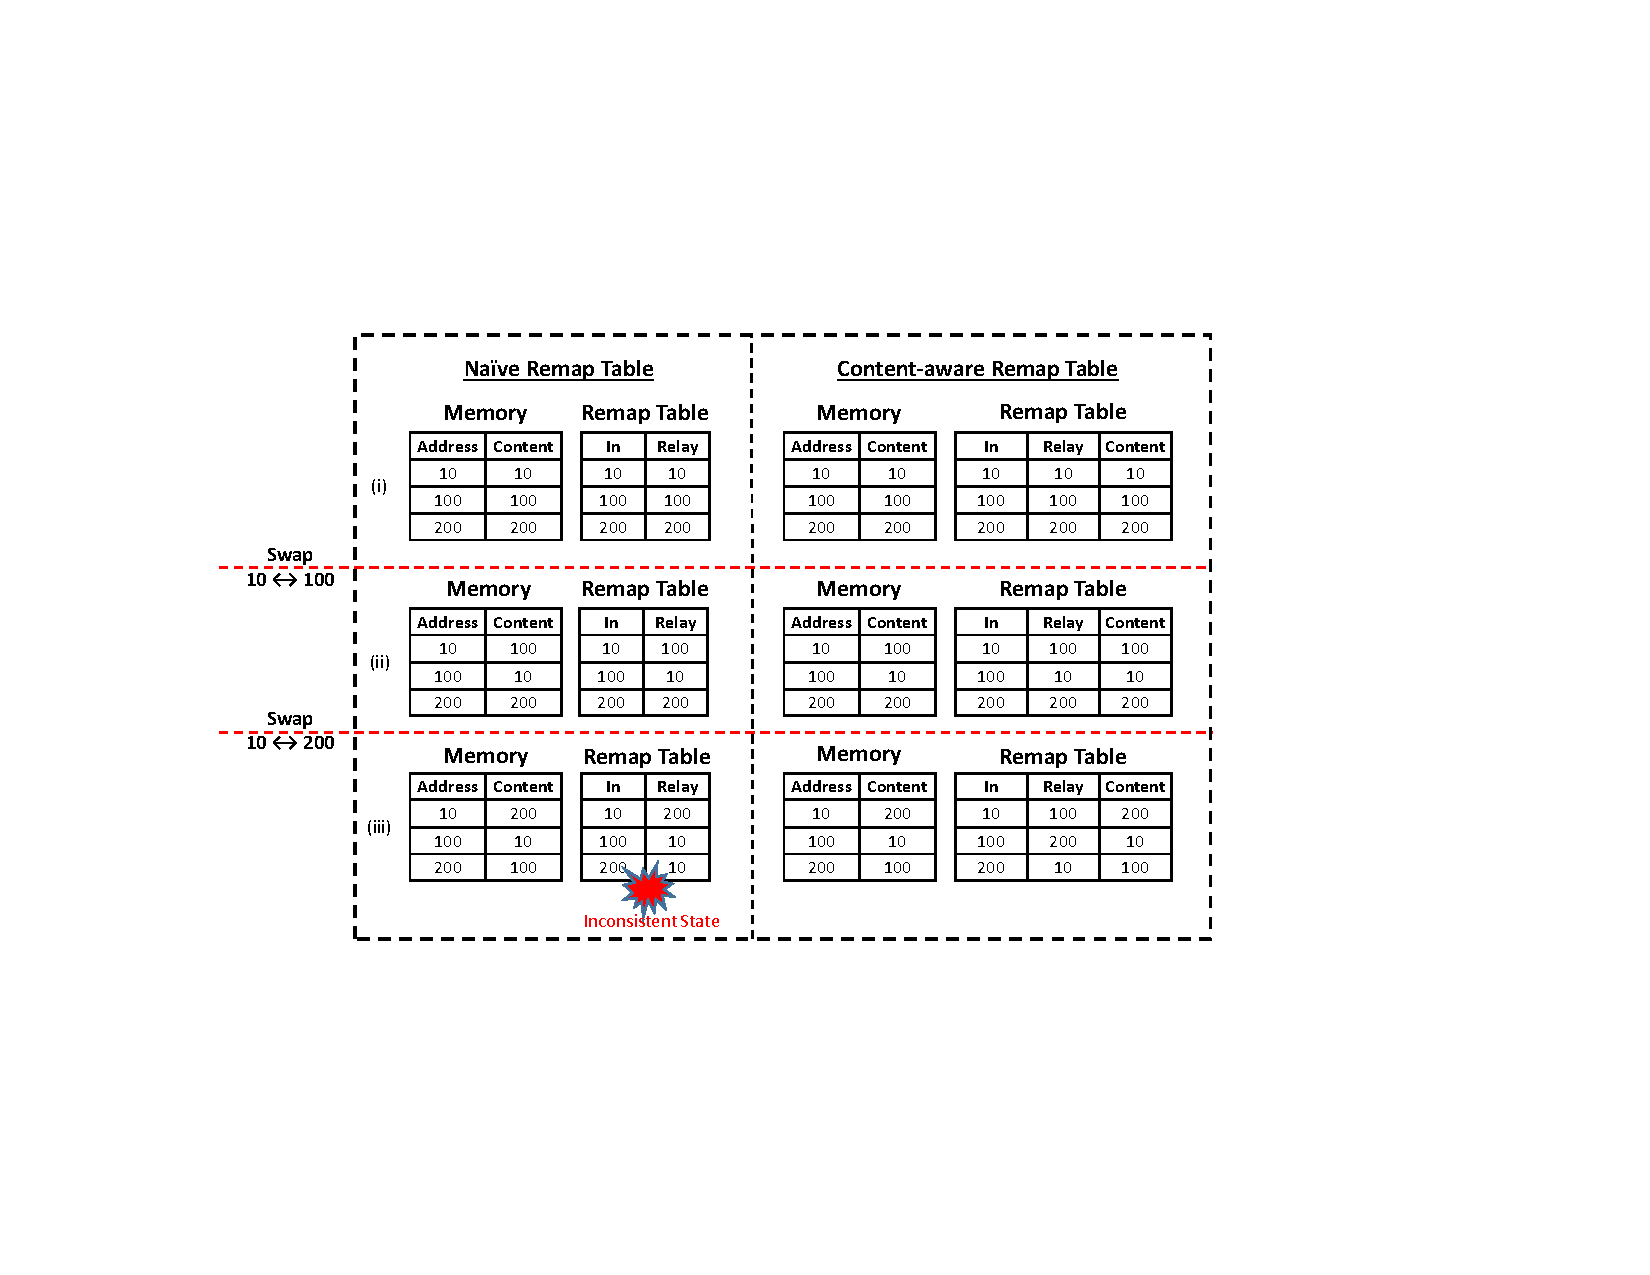
\includegraphics[width=0.46\textwidth]{figures/remap_table_design.pdf}
  \caption{Naive Vs content-aware remap table operation}
  \label{fig:remap_table_comparison}
\end{figure}

The first row shows the starting state of our memory before any migration, as well as the starting state of the two remap tables. For simplicity, we only present the three memory locations needed by our example. Page 10 is assumed to be a fast memory page, while pages 100 and 200 are slow memory pages. The numbers inside the memory locations represent the content page's id. The second row shows the states of memory and remap table after swapping pages 10 and 100. The content of page 10 is now page 100, and the content of page 100 is now 10. The naive remap table correctly states that requests to page 10 should be relayed to page 100 and vice versa. Everything works as it should during this first migration, however the third row shows the state after the second migration. Page 10 is now swapped with page 200. Such a migration would imply that page 100 (now held at 10) became cold and page 200 became hot. The contents are swapped and now page 10 holds page 200 and page 200 holds page 100. However, the state of the remap table is inconsistent. A request to page 10 would get forwarded to page 200, returning the wrong page. The right-hand side of Figure \ref{fig:remap_table_comparison} demonstrates the operation of a content-aware remap table able to support re-migration by updating the content page's remap table entry at each migration.

The naive remap table design fails simply because pages are allowed to re-migrate -- like page 10 in our previous example -- while the remap table ``assumes'' the content held at a page address matches the page's ID.  There is only one solution to this problem: The migration logic needs to be aware of exactly where each page's contents are located at any given time. Such a requirement can be implemented in various ways:

	\textbf{Safe and slow:} Always restore a forwarded page's contents to its original location before it participates in a new migration, resulting in two migrations instead of one. %For such an implementation, hot page count will have to be kept based on the content page instead of the real page Id. In the earlier example in Figure \ref{fig:remap_table_comparison}, the second migration of page 10 implies that page 100 is cold, but in order to offer page restoration support, the second swapping of page 10 will have to imply that page 10 is cold. The cold page (10) will be restored back to address 10 from 100 and then moved to its new location. Minor modifications are required to track activity based on the content page's id, that does not affect any other aspect of a migration mechanism.
}

	\textbf{THM approach:} Migration is restricted in ``segments''. In a memory configuration with a 1:8 fast:slow memory capacity ratio, each segment will have 9 pages; one in fast memory and the rest in slow. Each segment's 9 pages compete for a position at the one fast memory page available. This solution is elegant enough to allow re-migration with low storage overhead, limiting however the migration potential. If two or more hot pages coexist in a segment, only one can reside in fast memory at any given time. At the same time, if none of the segment's pages are hot, the fast memory page slot cannot be utilized by some other segment's page. %THM requires $\sim$5.6MB for its \textit{Segment Remap Table}.

	\textbf{HMA approach:} Any page can migrate to any other page address without the need of a dedicated remap table structure. The OS-based migration scheme imposes no limitations, as the OS takes care of updating the page tables and flushing the TLB. However, OS intervention and the penalties incurred due to cold TLBs can lead to high overheads.
	
	\textbf{MemPod approach:} Migration is restricted to be within a Pod,
Each Pod uses a remap table to allow page re-migration.  In addition to the
remap table, our algorithm also needs to identify all pages currently 
mapped to fast memory (to identify a candidate to be evicted in favor of a
new hot page).  We do this with a smaller, inverted table that gives the 
original address of each page currently mapped to fast memory.
 
%During the second migration in our example in Figure \ref{fig:remap_table_comparison}, the issue was caused because we updated the remap entry of the holding page (10) instead of the entry of the content page (100). An attempt to recursively follow the remap table's entries until we determine which one to update risks looping infinitely because of cycles (e.g., if page 10 is re-migrated back to address 10). Even if a smart algorithm is utilized to delete entries of non-migrated pages, the complexity of the recursive algorithm will only be bounded by the size of the remap table as, in the worst case, the entire table will be traversed. It's important to note that a content-aware remap table entry now points to a pair of values: (1) \textit{relay address} (where the requested page is located) and (2) \textit{content address} (which page is currently held). %MemPod requires 8MB per Pod and 32MB total for its sontent-aware remap table structure.

Recent works \cite{ramos-small-rt} propose other alternatives, as well.
They use arbitrarily small remap tables. When the remap table inevitably fills up two possible solutions exist: (a) migration is disabled or (b) the OS is invoked to update page tables and flush the TLB. After OS's intervention, the remap table is cleared and migration remains active.
%\end{description}


%\begin{figure}[h]
%  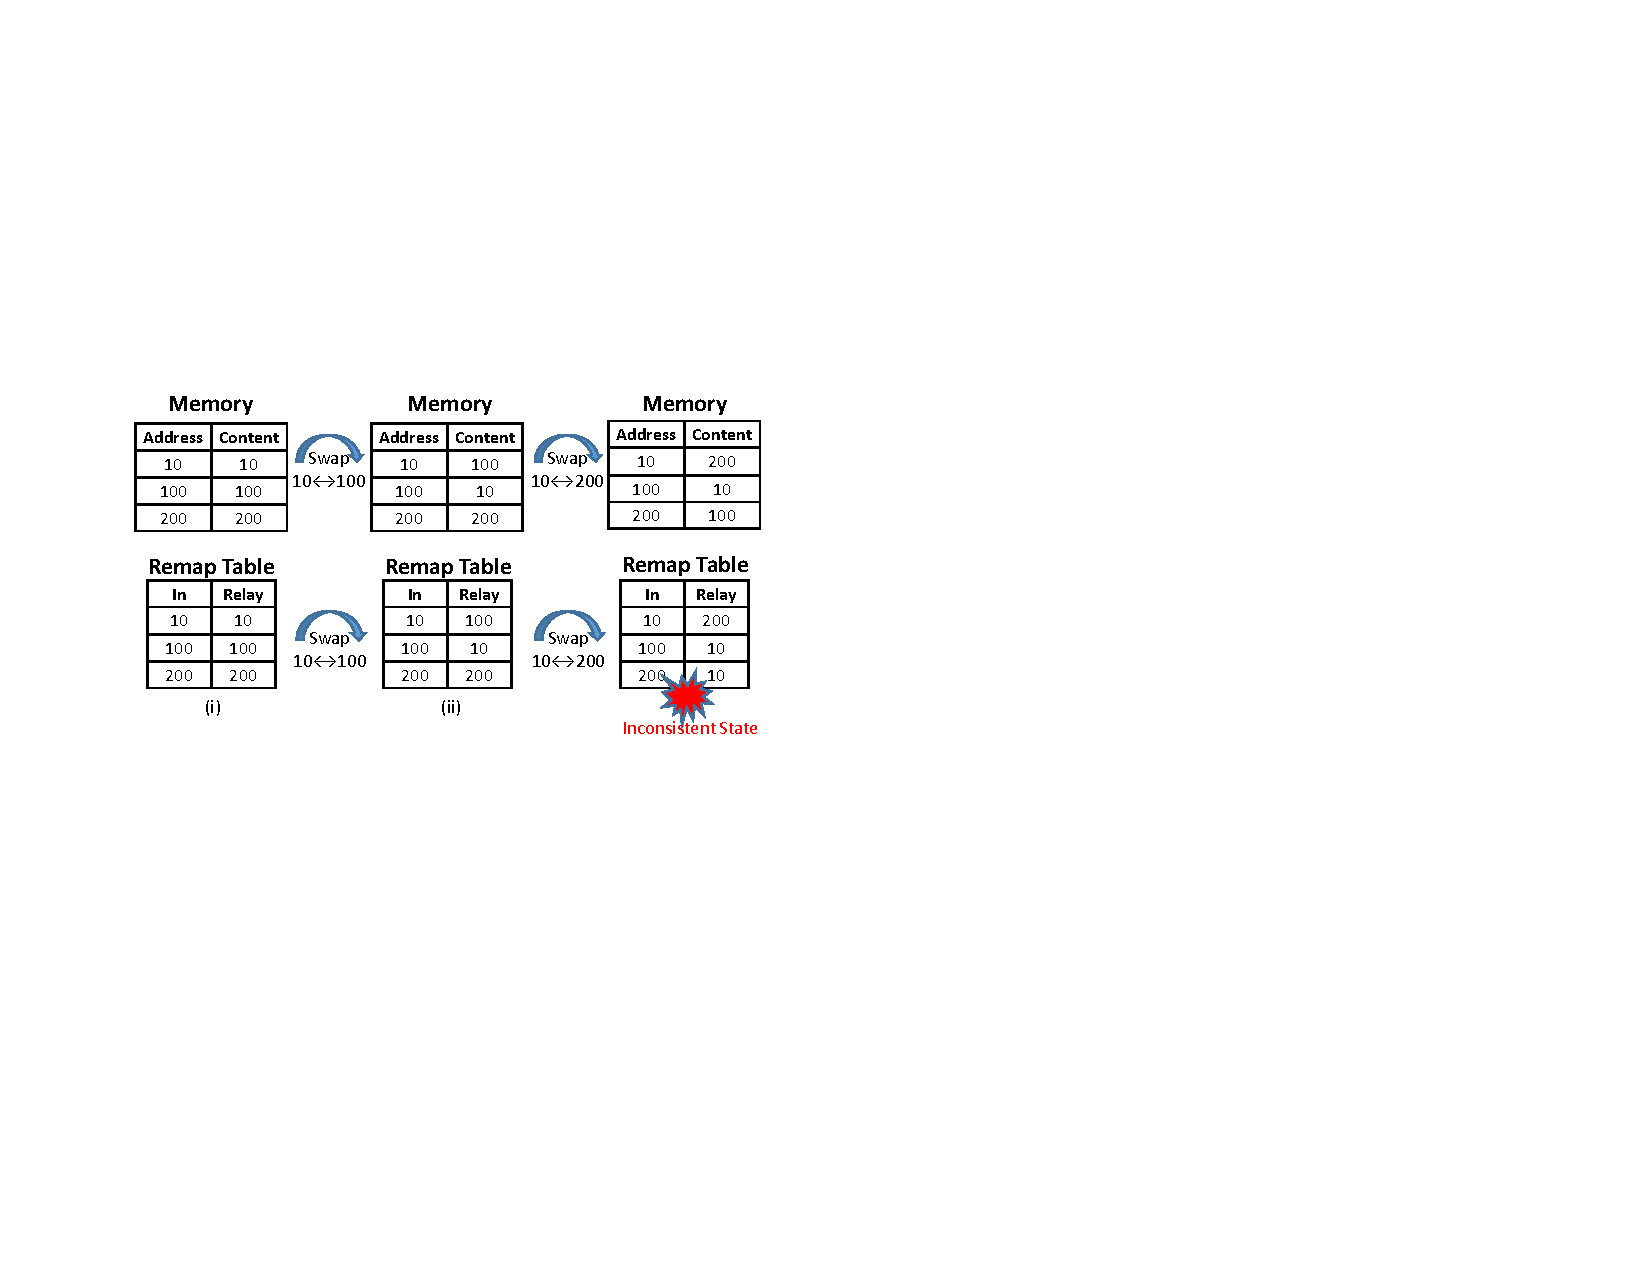
\includegraphics[width=0.46\textwidth]{figures/naive_remap_table.pdf}
%  \caption{Naive remap table operation}
%  \label{fig:failed_remap}
%\end{figure}
%
%\begin{figure}[h]
%  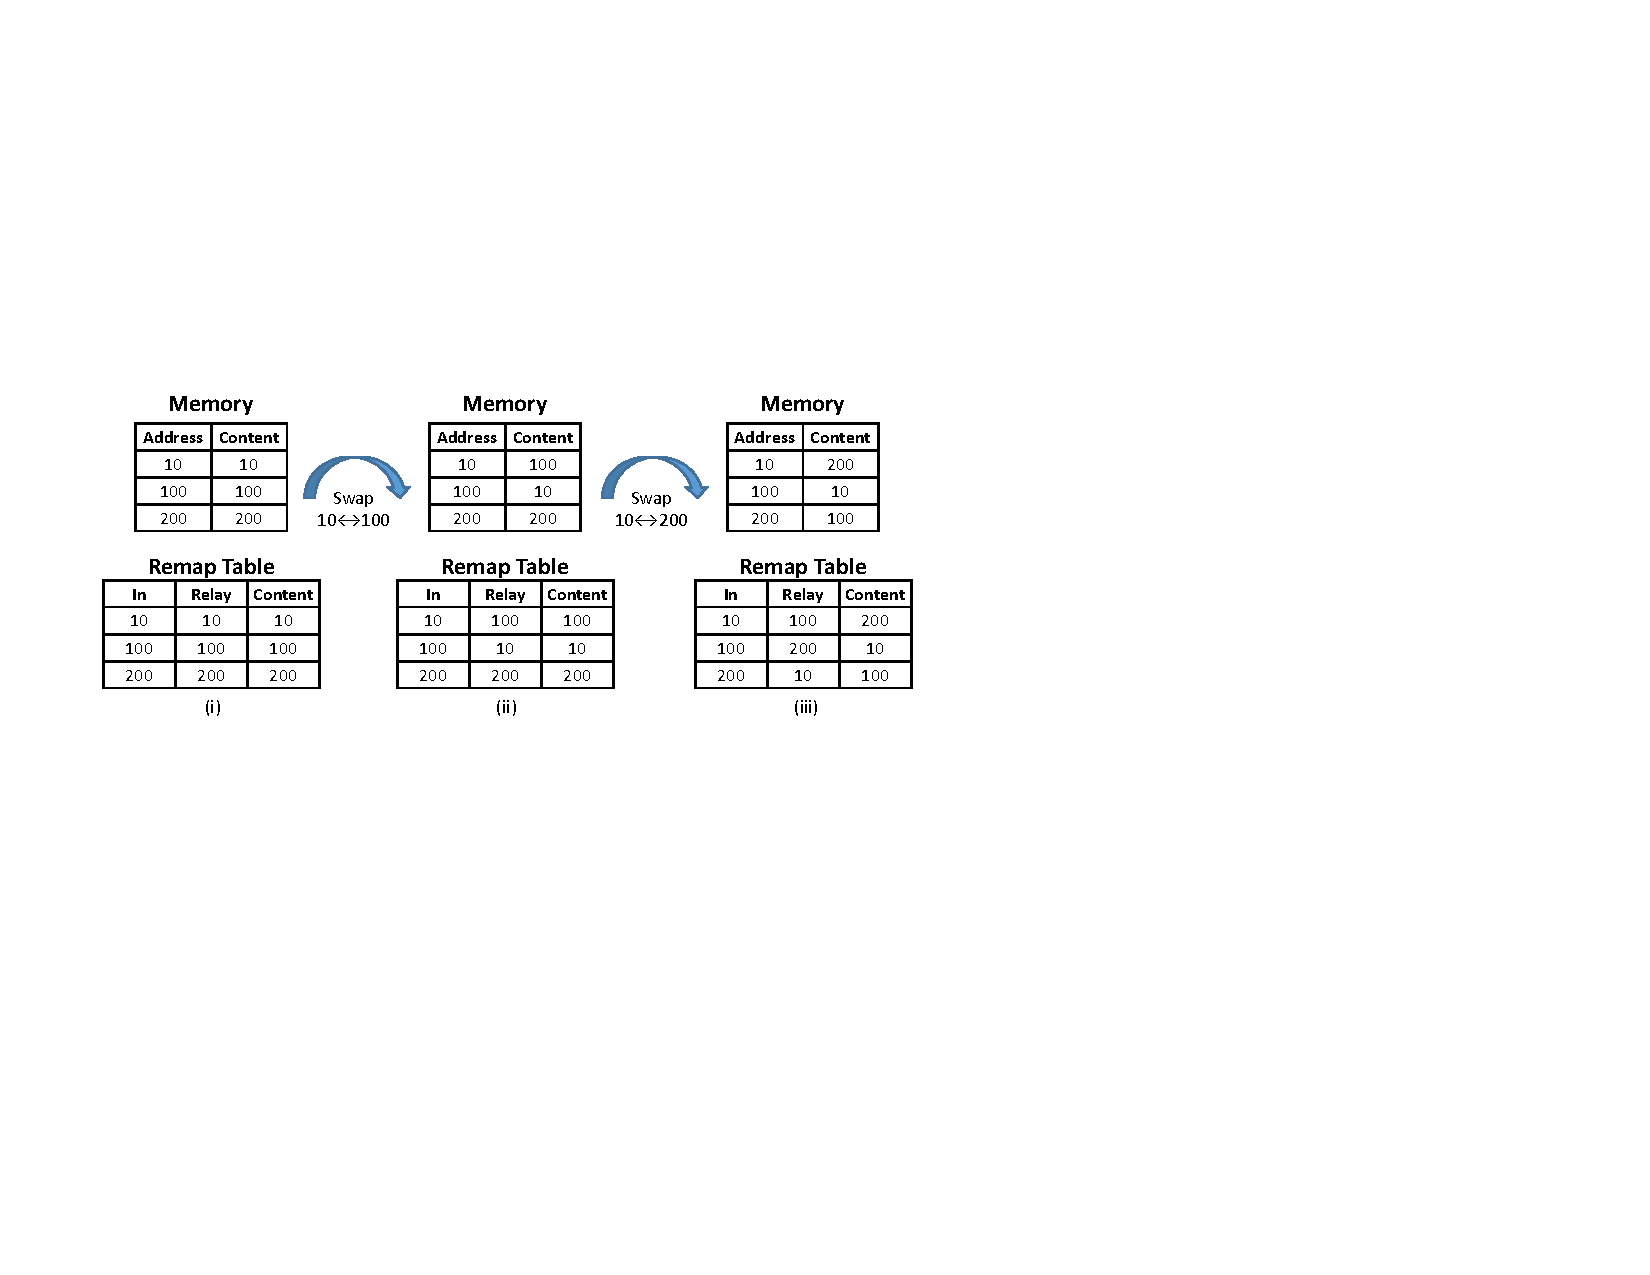
\includegraphics[width=0.46\textwidth]{figures/consistent_remap_table.pdf}
%  \caption{Remap design that allows re-migration}
%  \label{fig:correct_remap}
%\end{figure}


\subsubsection{Activity Tracking}
\label{sec:tracking}

Activity tracking is a critical element of any management mechanism for hybrid memories. In most studies on the subject, activity tracking becomes a synonym for identifying hot regions by counting the number of accesses to each one. In a more generalized approach, it could potentially be extended to track patterns, parallelism, bit flips/faults or any other information useful to the underlying mechanism. %Along with the remap structure, activity tracking is the limiting factor for most memory management mechanisms. The overhead of maintaining a set of counters per memory page (or any other granularity), is often a bottleneck. 

%MemPod utilizes an important observation to maintain a low activity tracking cost. Moving the hottest pages of an on-going interval into fast memory is a commonly accepted prediction technique, but not necessarily optimal. Several scenarios expose the failure of such an approach. For example, a page might become cold soon after it's migrated, wasting a space in fast memory. Another example arises when interval based migration policies are used. A cold page of the previous tracking cycle could become hot during the next interval. Strong indications exist that a combination of temporal as well as spatial locality has the potential of exposing better results. Our results in Section \ref{sec:MEA} demonstrate how Full Counters often conclude on a non-accurate prediction.

The overhead of maintaining a set of counters per memory page (or other granularity) will be high. Space requirements will increase linearly as memory capacities grow and the cost of sorting all the counters can overshadow any potential benefits in performance. Furthermore, our evaluation presented in Section \ref{sec:MEA} demonstrates that using full counters to ensure 100\% accurate counting may still lead to poor prediction accuracy. Frequently encountered cost-reducing solutions in the literature consist of increasing the activity tracking granularity in order to reduce the number of counters needed (i.e. track a group of pages together), limiting the bit width of counters, and caching a subset of the tracking state while the full set resides in main memory. 


%MemPod's activity tracking  is designed with a novel approach, using MEA to predict the hottest pages at a low cost. To the best of our knowledge, such an algorithm was never used in this context. THM also presents an interesting tracking approach, by utilizing competing counters for each segment.

%Using counters for every memory segment supported by the migration mechanism obviously imposes extremely high area overhead but benefits in \textit{counting} accuracy. Identifying the hottest pages however, also requires the often-overlooked sorting complexity. With the introduction of new memory technologies and the continuous capacity increase in memory capacities, it won't be long before even the most efficient sorting algorithm will require more time than we are willing to spend.

%\begin{description}
	\textbf{THM approach:} One 8-bit competing counter tracks each memory segment. A segment's competing counter is incremented by one when a page in its slow memory is accessed and decremented by one when the segment's fast page is accessed. The counter's value can then trigger migration when it exceeds a dynamically-set threshold. A ``monitoring region'' of memory where migrations are disabled is used by THM in order to update threshold values. Competing counters represent a trade-off between area overhead and accuracy and are susceptible to some error, as a cold page accessed at the right moment could trigger a migration and be placed in the fast memory.

	\textbf{HMA approach:} Full activity tracking per OS page (4KB) for all memory regions. HMA uses the least efficient tracking mechanism in exchange for perfect counting knowledge at a fine granularity. Full activity tracking also introduces the complexity of sorting all the counters to identify hot pages. THM and MemPod do not require explicit sorting.
	
	\textbf{MemPod approach:} MemPod requires an MEA map structure of K entries, where K is the number of hot pages we wish to identify at each interval. Our evaluation presented in Section \ref{sec:Results} finds a good number of MEA counters to be 128. Each entry maps a page's address to a counter. Through our evaluation, we identified a good counter size to be 4 bits and 21 bits are needed to address each page within a Pod, leading to a total storage cost of 1.56KB. Using the MEA counters, MemPod's activity tracking profiles \textit{all pages in memory} with minimal hardware cost. 

	
%As described in Section \ref{sec:MEA}, MEA is guaranteed to return the set of K hottest pages under certain assumptions that are not commonly held in a stream of memory requests. As demonstrated, MEA strikes a balance between most frequently occurring and most recently used page addresses, a fortunate and welcomed consequence in locality exposure. A new limitation arises when MEA counters are used: The system will be presented with the set of K hottest pages, however the counters' values cannot provide an order. The hottest page could have a lower counter value than any other page.
%\end{description}

Less efficient designs need to cache some of their counters while the rest are stored in main memory to alleviate the area overhead. THM's segment-based 
counters are automatically cached along with their corresponding remap table entries in THM's ``Segment Remap Table'' (SRT) and restored whenever necessary, at the cost of a memory access. 
MEA cannot be cached as it updates \textit{all} counters on an access. 
However, the space needed by MEA is small enough to easily fit on chip,
and its size need not scale with increasing memory capacity (it scales with
the maximum desired migrations per interval times the log of the
memory per pod).

%(didn't understand the point of this paragraph) -- It is also important to note that activity tracking updates should be moved off the critical path. Extreme tracking accuracy is not necessary for correct operation of any migration mechanism. Even if the tracking mechanism is not as accurate as it could be, all memory requests will be able to retrieve correct information as long as the state of memory and remap structure are consistent. Updating a remap table entry however, needs to be performed accurately without any ambiguity to alleviate the risk of inconsistent state.

\subsubsection{Migration Triggers}

Each solution must decide when to perform migrations. 
Migrations add significant delays to a system and any penalties incurred should be amortized by the performance improvement from placing a page in the fast memory. Requests that arrive while migrations are being performed have to be delayed to ensure functionally correct memory behavior. Throughout the literature, two triggers are most commonly used whenever state must be updated based on tracking information (MC scheduling, migrations, dynamic voltage and frequency scaling etc.). Interval-based (or epoch-based) triggers occur with a set frequency, while threshold-based solutions trigger whenever a predetermined criterion is met. 
Both interval-based and threshold-based approaches face the same challenge of identifying the optimal interval or threshold value. 
%(this just all seems too obvious to state)  -- Factors like a system's architecture, application's behavior, as well as semi-random factors (for example higher temperatures can lead to more frequent DRAM refreshes) make the optimal value differ from system to system. Designers usually opt for the value that provides the best results on average. The optimal value should not be too small as it will trigger some potentially expensive procedure frequently, but it cannot be too large as that reduces the ability to adapt to application phase variations. 

%As far as memory migration in flat address spaces is concerned, the state-of-the-art mechanisms trigger their migration procedures based on:
%\begin{description}

	\textbf{THM approach:} THM uses a threshold-based mechanism. When the competing counter described in section \ref{sec:tracking} exceeds a threshold value, migration is triggered. THM will swap the page that triggered the event with the page currently residing in the segment's fast memory page. Each segment can trigger migration independently and asynchronously since no interval is used. THM risks very frequent migrations that will stall the stream of incoming requests until each swap is finished. To overcome this issue, THM dynamically predicts the expected benefit of using one threshold value from a set of four pre-defined values. A ``sampling region'' of memory where migrations are disabled is used allowing THM to extrapolate and associate a potential benefit with each one of the pre-defined threshold values. When THM expects that migration costs will be amortized it updates the threshold value.
	
	\textbf{HMA approach:} HMA uses an interval based mechanism. Upon each interval, HMA attempts to migrate enough pages to fill the entire fast memory. However the high cost associated with OS intervention, management, and the penalties of a cold TLB favor long intervals. HMA authors identified the optimal timing interval to be as high as 1ms.
	
	\textbf{MemPod approach:} MemPod uses timing intervals. At each interval a Pod will migrate up to K pages into its fast memory, where K is the number of MEA counters used. MemPod is transparent to the system, rendering costly OS intervention unnecessary. Since each one of the N Pods will attempt to migrate up to K pages, up to N$\times$K migrations can happen within each interval. However, all Pods can perform their migrations in parallel. %The time required by MemPod to execute N$\times$K migrations is equal to the time to execute K migrations.
	
%\end{description}

\subsubsection{Migration Datapath}

Regardless of the choice for each migration building block described so far, once migration is triggered, the migration manager has to follow these 
steps. First, migration candidates need to be identified. Traditionally, one page (or a segment depending on the migration granularity) from the slow memory and one from fast memory. The two identified candidates need to be swapped. First one or both pages will be read and stored in temporary buffers and then written at their remapped locations.

%Describing the actual migration datapath is often overlooked in migration publications. 
Without dedicated page migration driver hardware, migration will have to be orchestrated by the OS and CPU cores. Consequences include communication delay, 
potentially some pollution of the processors' caches 
and the unavailability of those CPUs during migration. 

MemPod implements the migration driver within each Pod. As the Pod has direct communication with the MCs, added delays are kept to a minimum,
and no traffic is generated at the global switch (saving energy and eliminating contention).
%and the CPUs are free to keep executing non-memory instructions. 
In HMA, the OS orchestrates everything. Some CPU cores have to be stalled and used to service the OS interrupt, causing the migrated pages to traverse through communication mediums and caches on each way. THM does not fully describe its datapath, but it appears that CPUs are used in this case as well. 
However, to make a generous comparison, we do not model the penalty introduced by using CPUs for migration in our HMA and THM simulations presented in Section \ref{sec:Results}.

%We assume that channel parallelism is utilized when reading and writing the candidate pages. In other words, the two read commands will be sent in parallel, as well as the write commands that follow. Consequently, The hardware penalty for one page swap is the time required to read an entire page from and then write it to the slow memory. We also assume that writing the two candidates back incurs row buffer hits since the page was just opened in the previous step. In this study, we evaluate all mechanisms under the same memory organization and as such, the memory time required for one migration is the same across all mechanisms. However, each mechanism introduces some unique penalties:
%\begin{description}

	\textbf{THM} does not introduce a cost for identifying the candidate pages as it follows a deterministic algorithm. The page that caused the competing counter to exceed the set threshold will be the slow memory candidate, while there is exactly one fast page candidate per segment.

    \textbf{HMA} attempts to fill the entire fast memory with migrated pages. The number of swaps that will be performed per interval can be as high as the number of pages in fast memory. Inevitably some hot pages will already reside in the fast memory and they will not be migrated to a different location in fast memory. 
%HMA introduces costs that are hard to estimate. 
HMA introduces several costs due to its software-driven architecture.
They include sorting all the activity tracking counters, traversing and updating page tables, flushing TLBs, and the cold-start effects of re-filling
the TLBs.
%We modeled HMA to not attempt migration of those hot pages. Such an approach could complicate finding a fast-memory candidate page, although with HMA's full activity tracking counters, and since sorting is a necessary operation at every interval, this problem can be reduced to the simple task of following the sorted activity list backwards (i.e. It's easy to find the coldest fast-memory page). Unfortunately, HMA introduces costs that are hard to estimate. Sorting all the activity tracking counters, traversing and updating page tables and flushing TLBs is part of the cost introduced by the OS. On top of that, the effect of a cold TLB can penalize severely all running applications.

	\textbf{In MemPod,} with the use of MEA counters, identifying the fast-memory page candidate is as simple as checking that it's not part of the K hot pages. The identification algorithm starts at the very first fast memory location and iterates sequentially until it detects a page address that is not in the set of hottest pages. For the next migration, the identification algorithm simply continues from where it was left. If a hot page already resides in the fast memory it is ignored.

%\end{description}

\ignore{
\subsection{Scalability to Future Memories}

\remark{Nuwan's comment:\\I feel like this section has a lot of repetition from what was already stated earlier in this section. It could either be shortened quiet a bit or removed (but if we remove it, we need to make sure the references earlier in the paper about how we expect MemPod to be better for future memory systems aren't left dangling).}

As main memory capacities grow to terabytes, storing activity tracking information and remap tables in SRAM could become infeasible. Caching part of the migration logic and using part of main memory as backing storage will become necessary. MemPod's semi-distributed architecture allows caching without any coherence concerns as Pods never share information. %An analysis on the impact of such caching, as well as the optimal cache size is presented in the experimental evaluation section. 
\remark{Keep in mind that MemPod actually has the highest costs, according
to your tables, so it is actually going to suffer the most as capacity scales.}



\remark{Again, I just don't know yet why this is true...  
At such capacity levels, centralized migration controllers will no longer be sustainable due to the severity of the introduced request serialization penalty. Further, as applications become more data-centric, it's safe to assume that memory traffic would also scale up, as well as sustainable bandwidth expectations. }

Alternative approaches described in this Section limit the size of the remap table at the cost of disabling migration when full, or invoking the OS before migration resumes. This approach could also be incorporated in future migration mechanisms. We should note that with a limited remap table size, or even an available number of counters less than the number of fast pages, MemPod would still offer the potential of migrating \textit{any} slow memory page to the limited set of fast pages (as long as it's within the same Pod) available for migration, in contrast to THM, where only those segments that happened to fit in the new limited size will be able to migrate, forbidding migration of the rest of the slow pages. HMA would remain intact from this limitation since no remap tables are necessary.

\remark{I don't believe I saw those ``alternative approaches'' mentioned.\\A.P.: There was only one in the remap table subsection.}
}


















































% !TEX root = ../MemPod.tex
\section{Results}
\label{sec:Results}

\subsection{Evaluation Framework}
\label{sub:Evaluation}

The goal of our evaluation framework is to quantitatively and qualitatively assess MemPod's capabilities and compare it against state-of-the-art proposed mechanisms. Throughout our evaluation section, we study MemPod's performance running with an eight-core CPU. We extend Ramulator \cite{kim-ramulator} to support flat address space hybrid memories. We model the MemPod architecture,
as well as HMA, THM and CAMEO in our simulation framework. Ramulator enables 
cycle-level memory simulation and includes a simple CPU front-end capable of approximating resource-induced stalls. We chose to evaluate MemPod under a realistic memory configuration consisting of 1GB 3D-stacked HBM \cite{JEDEC-HBM-REVISED} and 8GB of off-chip DDR4-1600. Table \ref{tab:specs} Provides a more detailed description of the simulated system's configuration.

\begin{table}[t]
  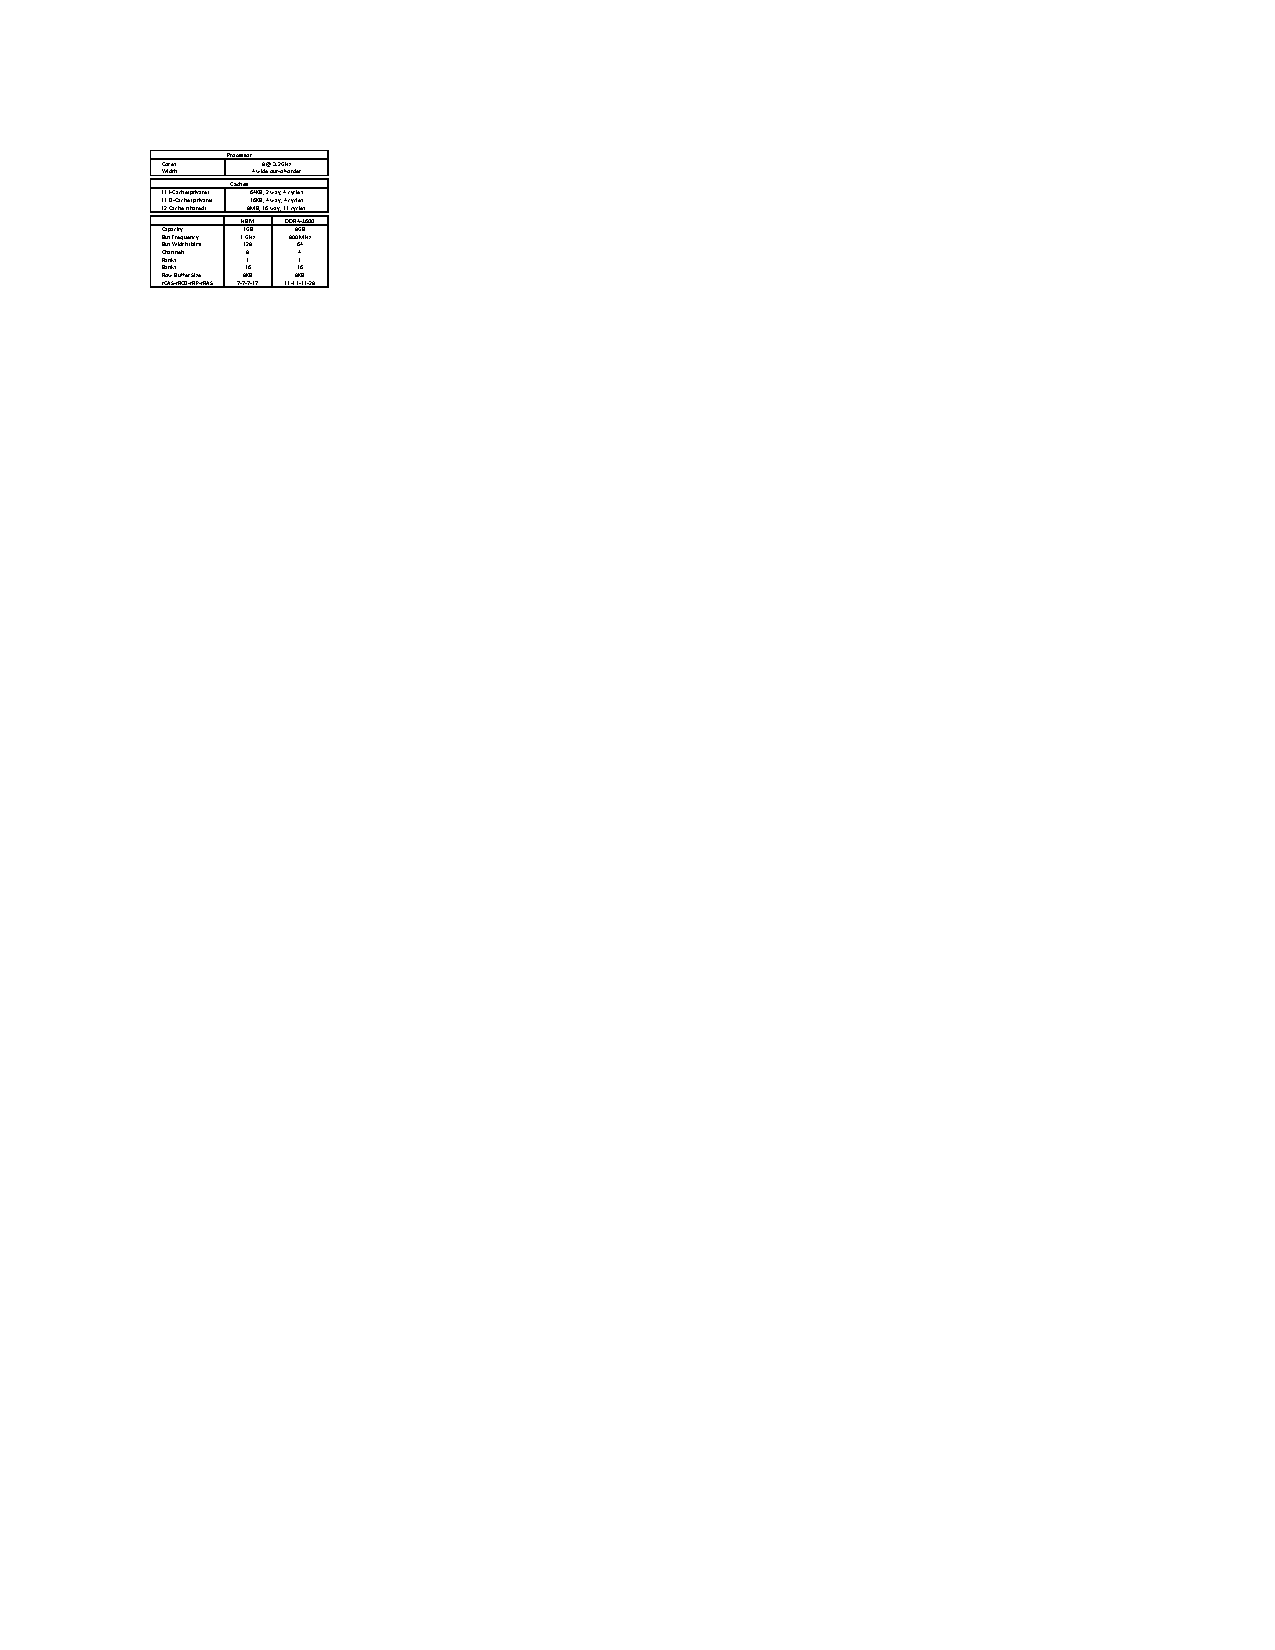
\includegraphics[width=0.46\textwidth]{figures/specs_table.pdf}
  \caption{Experimental framework configuration}
  \label{tab:specs}
\end{table}

\subsection{Experimental Methodology}
\label{sub:Experimental}

We use benchmarks from the SPEC2006 suite \cite{spec} as our workloads. Using Sniper \cite{sniper}, we recorded memory request traces while simultaneously executing 8 benchmarks on a simulated 8-core CPU. We then feed these multi-programmed memory traces into Ramulator, executing all workloads to completion. Our complete set of workloads consists of 15 ``homogeneous'' workloads, where 8 copies of the same benchmark are run in parallel (we simply refer to these workloads by the benchmark's name in later results), as well as 12 workloads featuring a random mix of 8 benchmarks each (referred to as mix1-12). Each benchmark was executed and traced under its reference input. When running homogeneous workloads, Sniper ensures that memory pages are not shared between workloads. A breakdown of the mixed workloads is shown in Table \ref{tab:workloads}.

\remark {A.P.: I'm trying to point out that same benchmarks send memory requests to different pages.}

\remark{I guarantee reviewers are going to ask -- when running 8 copies, 
did you use 8 unique inputs?}

We also extended Ramulator with cacheing for the activity tracking and/or remap tables depending on the simulated mechanism. Cache misses inject memory requests into the stream of requests fed by our trace files to retrieve the missing information. No priority is given to these cache miss requests over regular requests. When caches for hybrid memory management techniques are disabled, the simulator assumes that any information needed by any mechanism exists on chip and is accessible without any delay. The migration process was implemented in detail as well. In order to read an entire 2KB DRAM page from memory, 32 read requests need to be sent for each of the two migration candidates and then another set of 32 requests for each of the two write-backs.

As we use Ramulator with recorded traces, we chose to report Average Main Memory Access Time (AMMAT) in our results. Even though Ramulator has the ability to approximate IPC with a simple CPU model, 
AMMAT is computed with much greater fidelity with this tool,
as it models the memory system in great detail. AMMAT is the average time 
spent accessing and waiting for main memory by each request (lower is better). Due to space limitations we are not able to show results for individual workloads in most of the graphs in this paper. In those graphs, we only present the average of all mixed workloads, average of all homogeneous workloads, and overall average.

In our AMMAT experiments, we typically introduce additional accesses to the
system (migrations, bookkeeping cache misses).  The overhead of the additional
misses is accounted to the total memory stall time, but the total memory 
stall time is divided by the number of original LLC misses (main memory requests) captured in our traces
-- that is, the denominator in our AMMAT equation does not change between
experiments and equals the number of requests in our trace file.

\begin{table}
  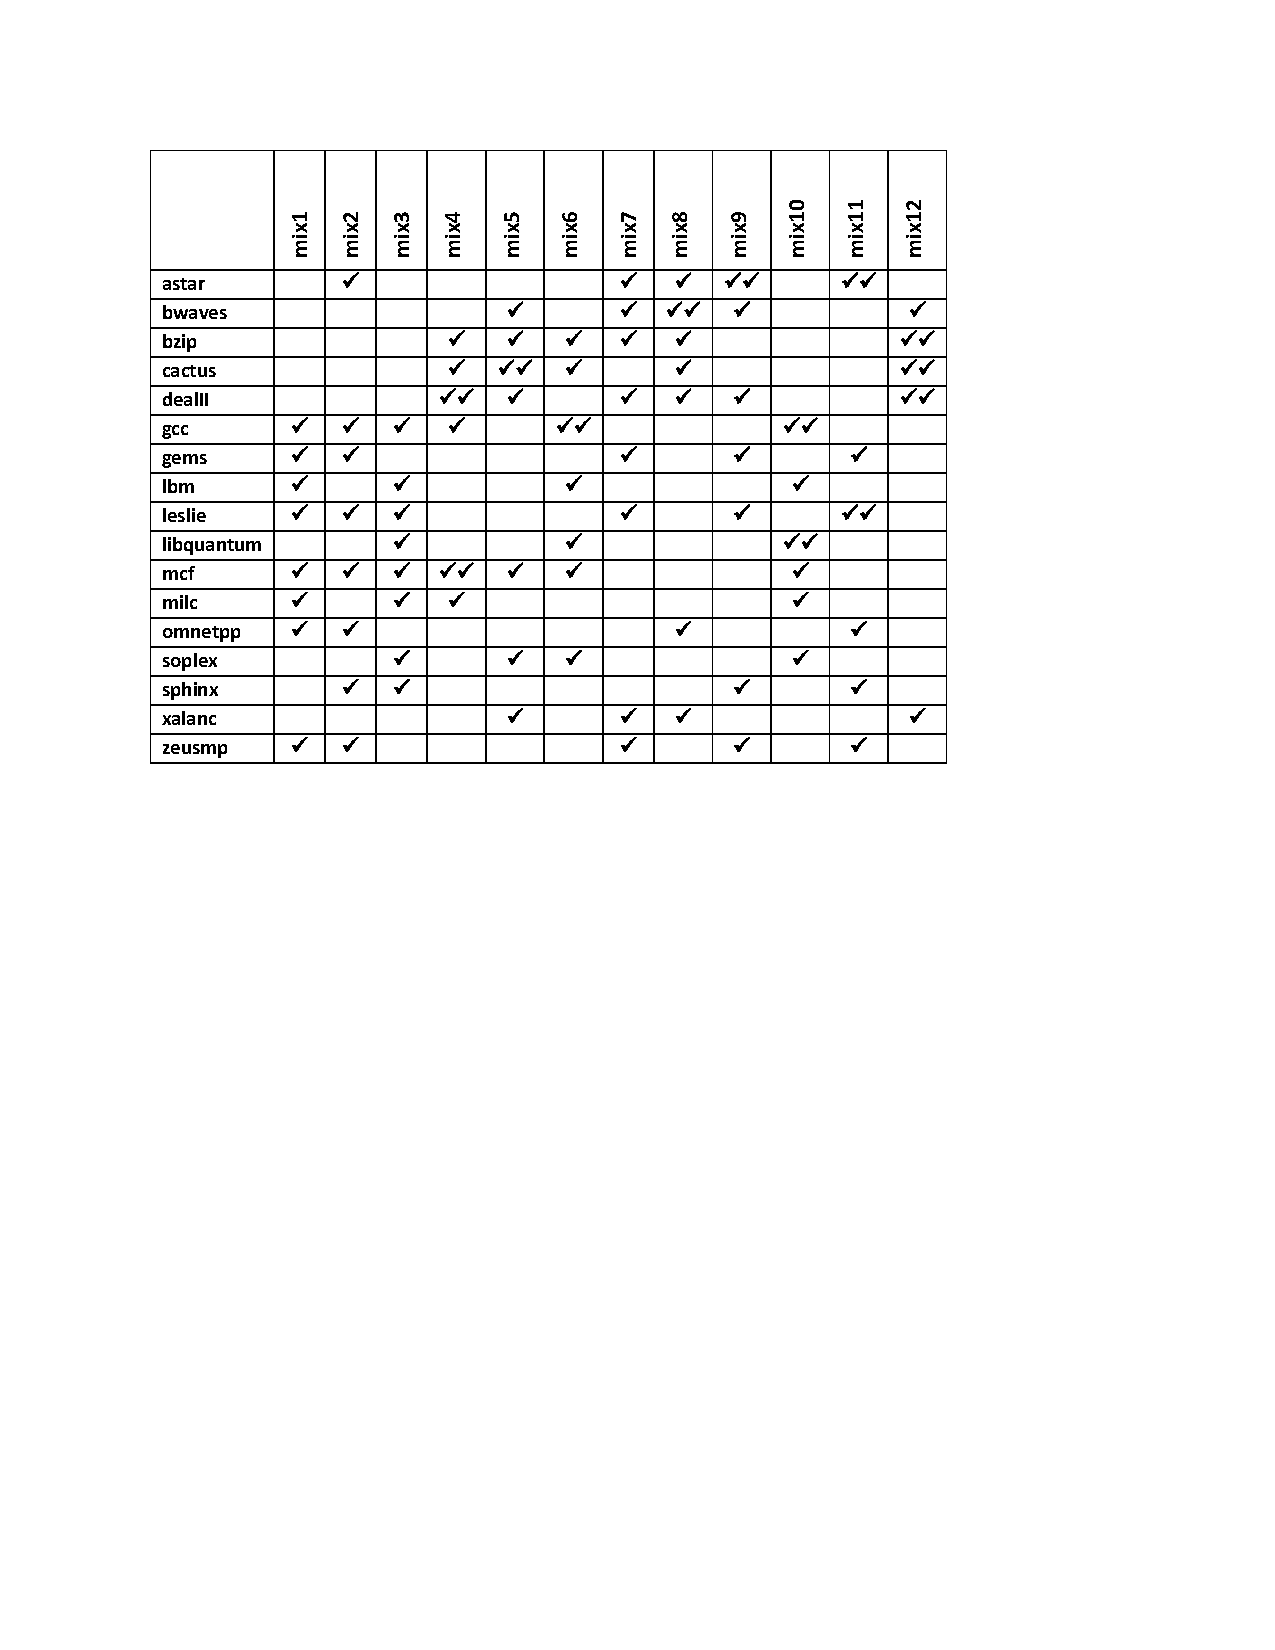
\includegraphics[width=0.46\textwidth]{figures/workloads_checkmarks.pdf}
  \caption{Mixed workloads description}
  \label{tab:workloads}
\end{table}

\subsection{Simulation Results}
\label{sub:SimResults}

\subsubsection{Page Tracking and Migration Design Space}

MemPod's activity tracking overhead and migration traffic is impacted by
the number and size of the MEA counters, as well as the epoch (interval) 
size over
which the counters accumulate.  We examine each of these design space
parameters in this section.
The number of MEA counters dictates the highest possible number of 
migrations that can be performed at each interval by each Pod, while the epoch length will determine MemPod's ability to better adapt to phase changes in a workload. The size of each MEA counter sacrifices accuracy when smaller counters are used 
but can also save space on the chip.  For these initial experiments,
the epoch length was 200$\mu$s. 

We first examine the number of MEA counters, by keeping the epoch length constant and exponentially increasing the number of counters from 16 to 512. In order to minimize the impact of other factors, we execute this experiment with 16 bits per counter and remap table caches disabled. 
%In other words, each counter was given more than enough space and all required information such as the remap table resides entirely on the chip and is accessible at no cost. 

Figure \ref{fig:num_counters} shows AMMAT normalized to the case when 16 counters are used, along with the average number of migrations per Pod per epoch (secondary axis). The results indicate that each Pod does utilize the higher number of counters and consequently perform more migrations per interval. However performance is degraded due to the overhead of migrations when more than 128 counters are used. Using 128 counters, AMMAT is improved by 6\% over the baseline with 16 MEA counters. 

\begin{figure}[h]
	\centering
  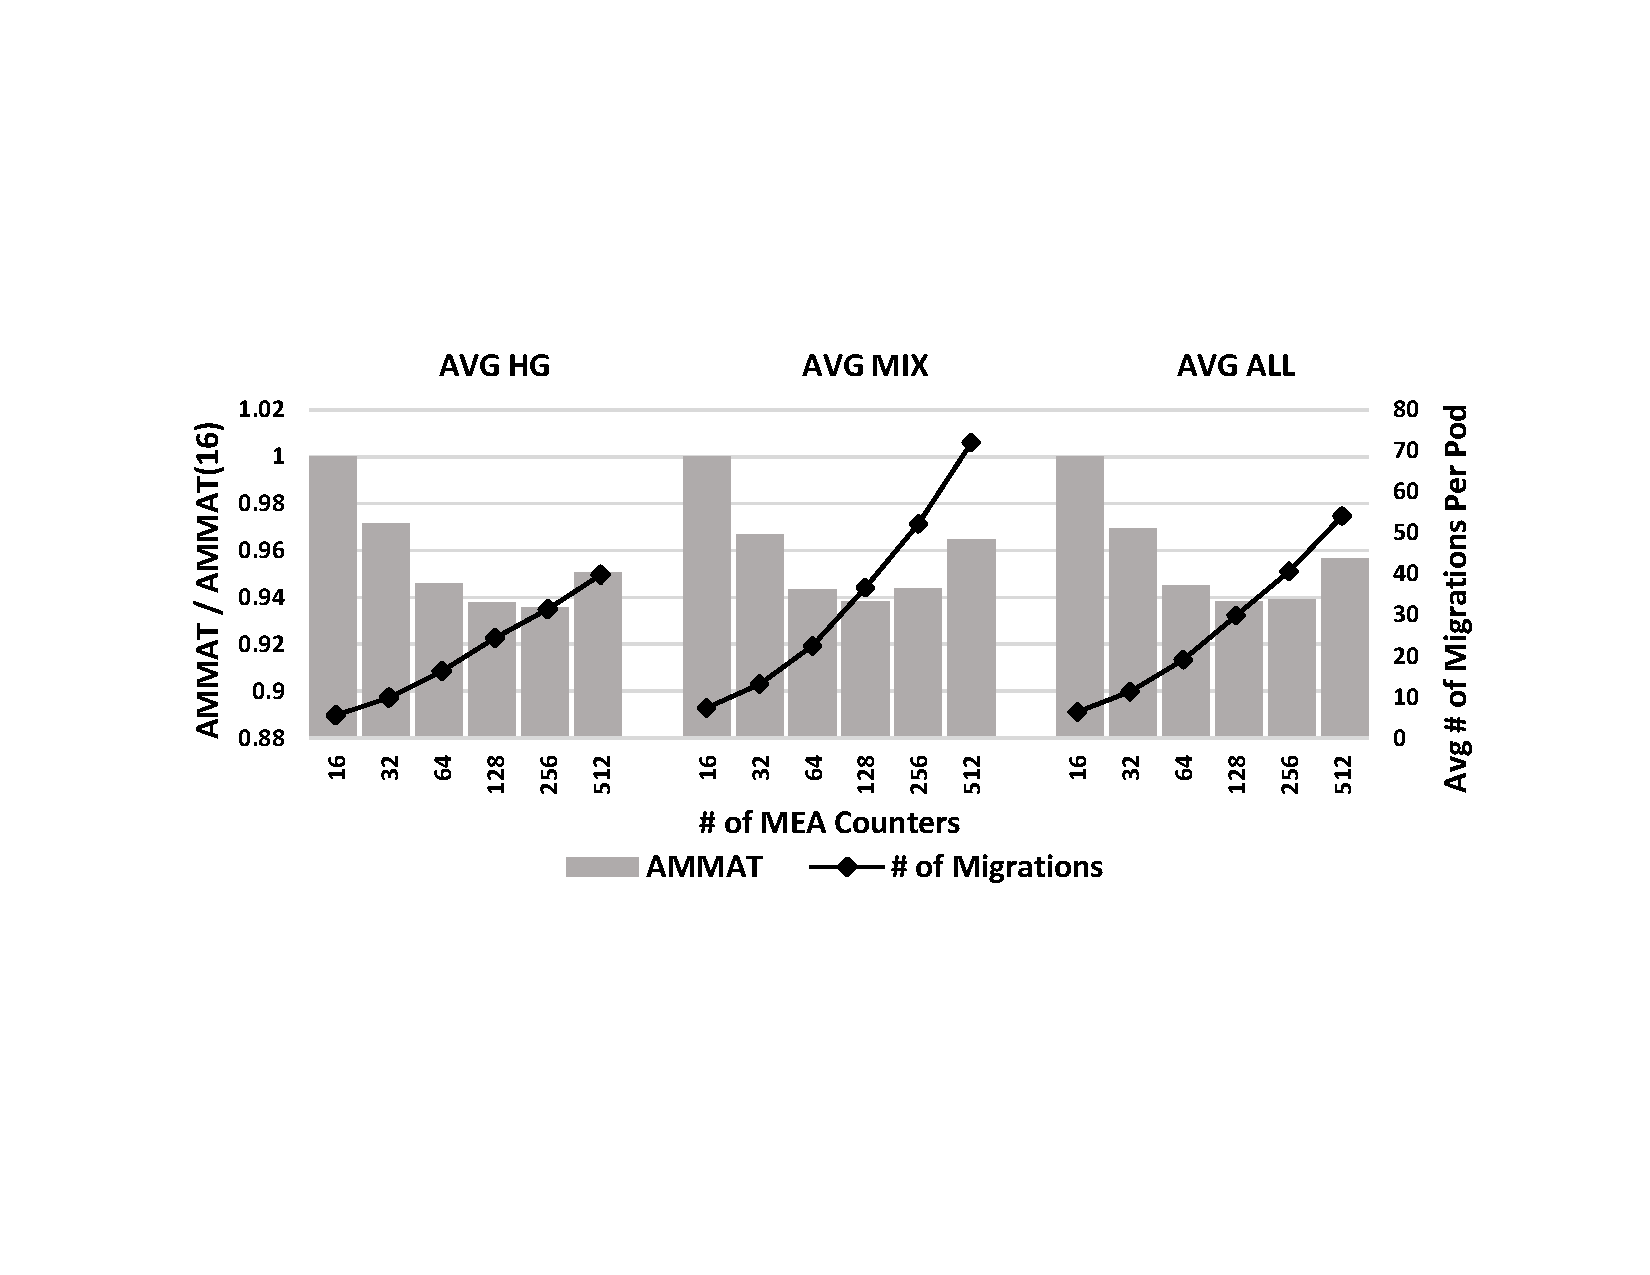
\includegraphics[width=0.46\textwidth]{figures/revised/old/num_mea.pdf}
  \caption{\# of MEA Counters Vs Normalized AMMAT (primary axis) and average \# of Migrations per Pod per interval (secondary axis)}
  \label{fig:num_counters}
\end{figure}

Figure \ref{fig:interval} shows the same experiment, but with a varying epoch length. Remap table caches were again disabled, each counter was given 16 bits and the number of MEA counters was set to 128. We observe that on average, MemPod reports the lowest AMMAT with interval length of 100$\mu$s (1.2\% improvement over 50 $\mu$s on average). As the interval length increases, more migrations are performed and AMMAT increases. Dropping below 100$\mu$s has a negative effect on AMMAT due to some epochs being entirely consumed by migrations. For comparison purposes, HMA \cite{meswani-HPCA21} identified the best epoch length to be 100ms (1000x larger) in order to support all the lengthy processes that take place during a migration event for that method.

\begin{figure}[h]
  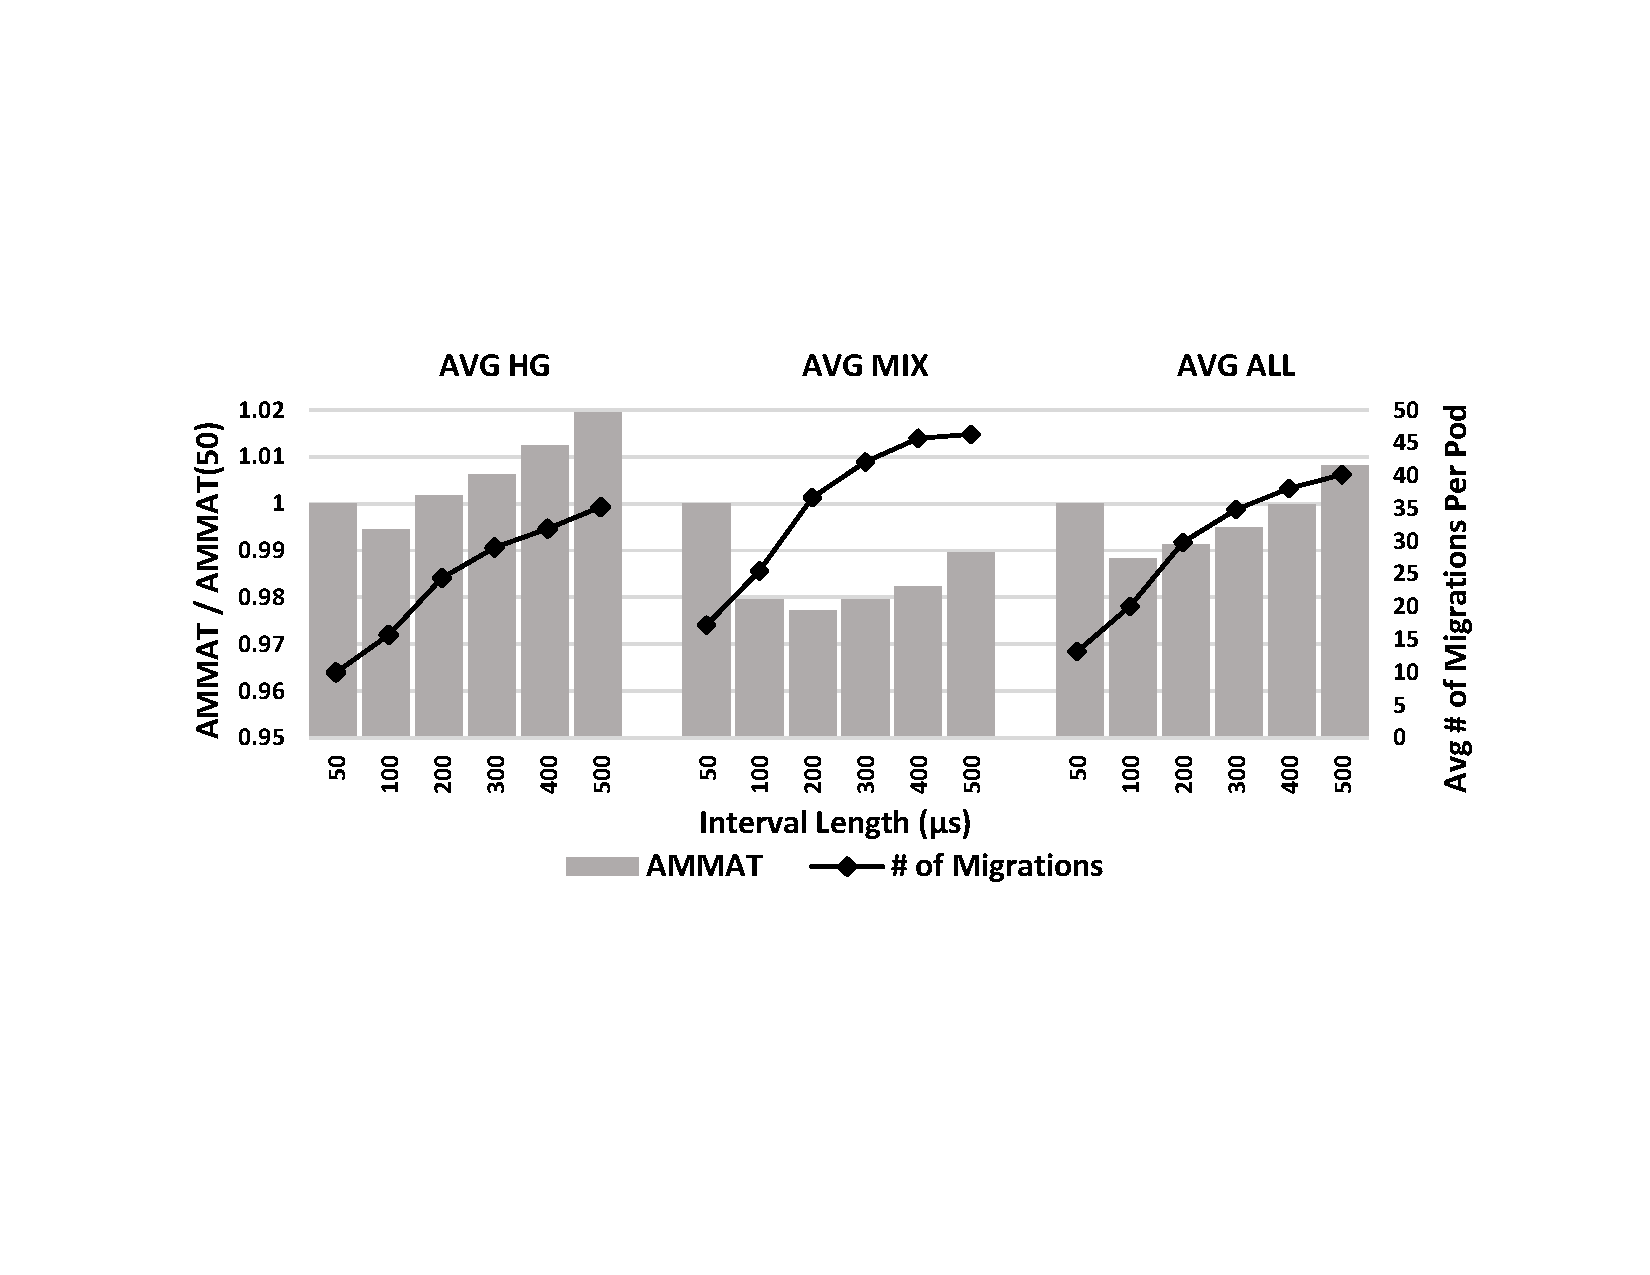
\includegraphics[width=0.46\textwidth]{figures/revised/old/interval.pdf}
  \caption{Interval Length Vs Normalized AMMAT (primary axis) and average \# of Migrations per Pod per interval (secondary axis)}
  \label{fig:interval}
\end{figure}

The size (in bits) of each counter defines the area requirements of our MEA tracking mechanism. \remark{Nuwan's comment on next sentence:\\I don't understand what this sentence is trying to say. Please reword/clarify. Why do we not saturate the counters instead of overflowing?\\A.P.: Not sure I understand this comment.} 
\remark{Dean -- my same question -- why don't we use saturating counters???}
%We modified MEA to remove map entries with counter values equal to or less than zero (instead of strictly equal to zero) in order to support counter saturation. We opted not to immediately remove an overflowed counter even though its value is now zero, as the existence of the correct counter set is crucial to the algorithm's accuracy. For this experiment we used the optimal parameter values identified in the previous experiments and set the number of MEA counters to 128 and interval length to 100us. 
%All caching was disabled in order to study the direct impact of this variable.

Figure \ref{fig:counter_size} presents the impact of counter size on AMMAT and average number of migrations. We see only minor differences in these results,
in large part because of the competing effects of accurate counting (with
large counters) and more temporal effects (with small counters).
The small counters better capture recency, because with small counters it
requires fewer divisions \remark{A.P.: Is ``divisions'' the correct word here?} to eliminate a high-access page from the pool and
replace it with a new page.  We do see a definite sweet spot at 4 bits,
where both effects seem to be in play.  We confirmed this by re-running the
experiments in Section~\ref{sec:MEA} with 4-bit instead of 16-bit counters,
and saw that prediction accuracy did improve slightly.  Although the marginal
gains are small, we use 4-bit counters in our subsequent experiments.


We first observe that 8 bits are sufficient for our workloads, as larger sizes report identical results. Our second observation is that two bit counters report a negligible performance degradation (0.3\% on average) \remark {A.P.: It's not a degradation over 8 bit counters but an improvement. Changed the sentence to compare with 4 bit counters but we might want to discuss the AMMAT improvement compared to 8 bit} over 4 bit counters and a reduced average number of migrations.

\begin{figure}[h]
  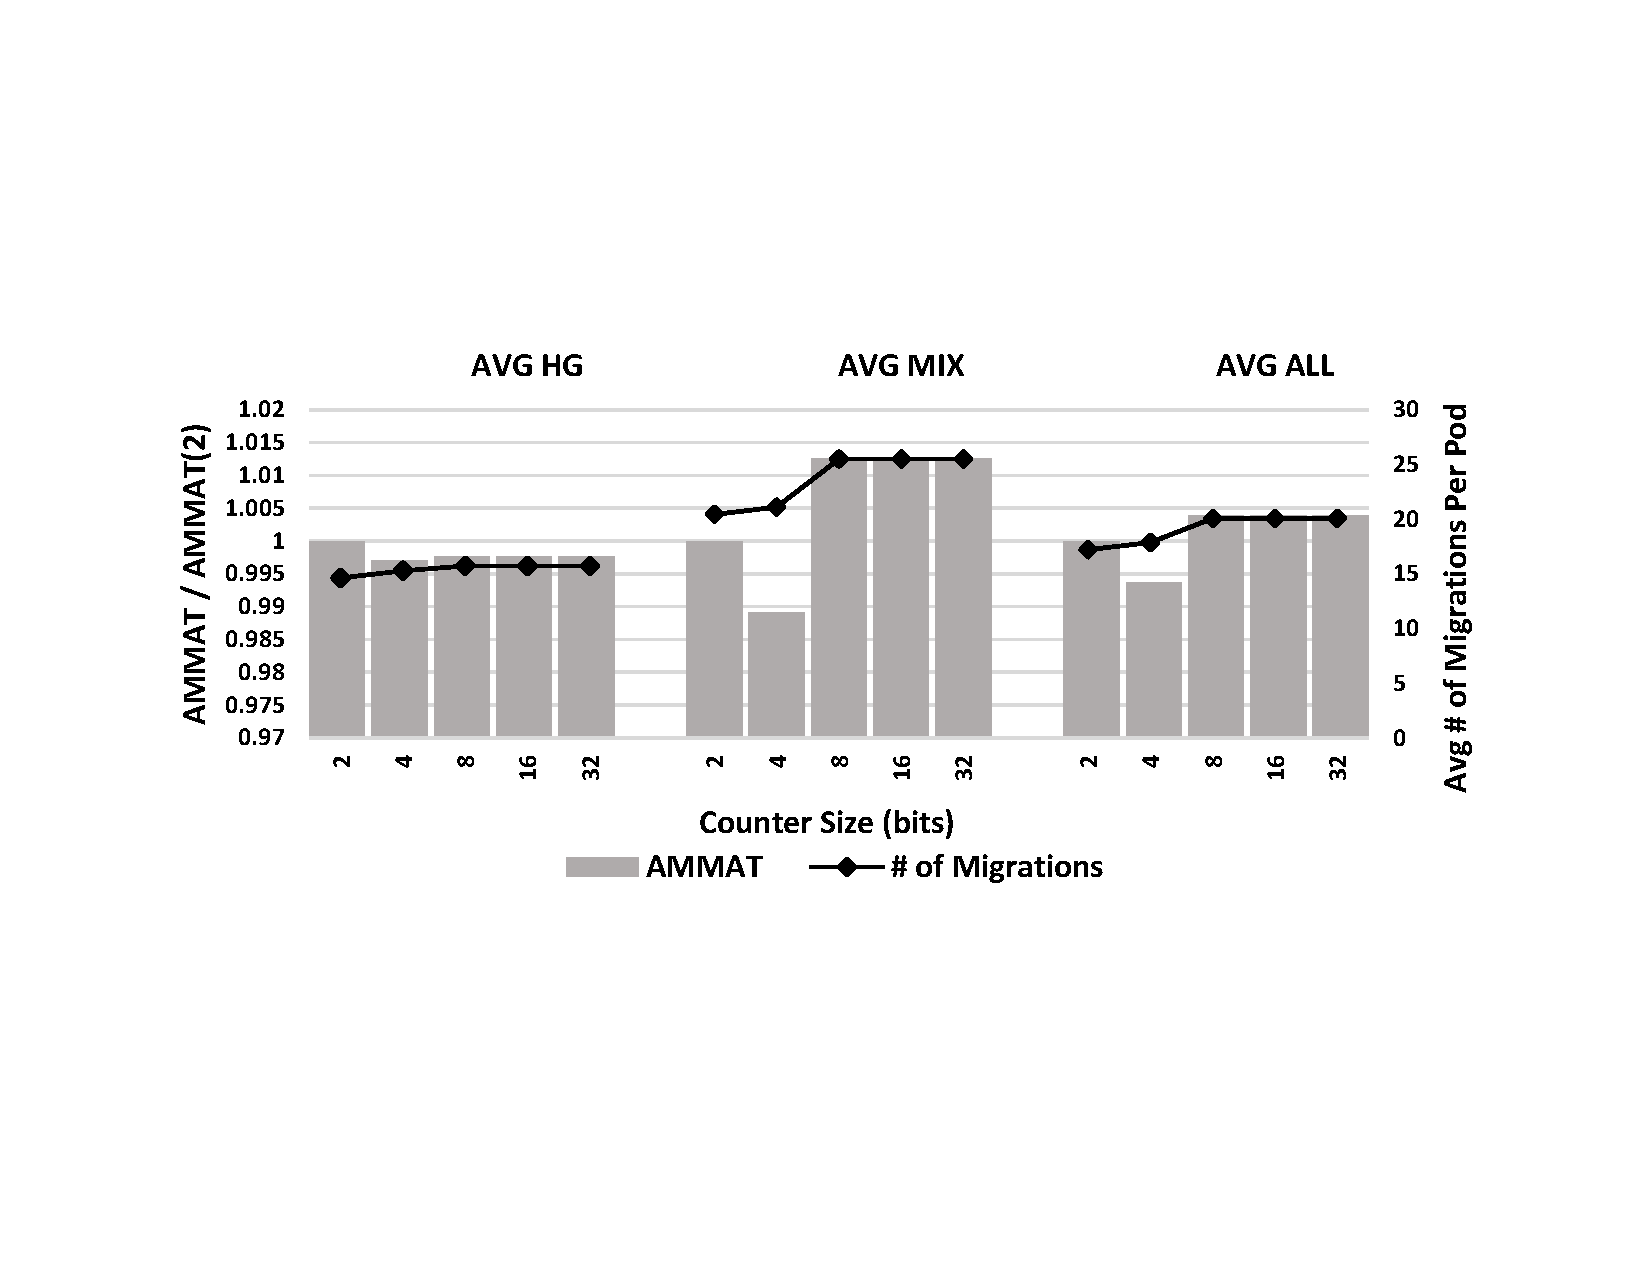
\includegraphics[width=0.46\textwidth]{figures/revised/old/ctr_size.pdf}
  \caption{Counter size (in bits) Vs Normalized AMMAT (primary axis) and average \# of Migrations per Pod per interval (secondary axis)}
  \label{fig:counter_size}
\end{figure}

The most interesting observation comes from assigning 4 bits to each counter. On average, performance is boosted slightly (up to 3\% and 0.6\% on average) even compared to using larger counters, while migration count is low. %Since a difference is observed, we can conclude that these smaller counters ``lose'' information that in turn benefits overall execution. The reported result is a welcomed artifact of the MEA algorithm combined with application behavior. 

Based on our results, we identify 4 bits per counter to be the optimal value. Each one of the 128 MEA entries needs 21 bits for addressing the 1.1M pages per Pod and 4 bits for its counter, leading to an area cost of only 400B (128 MEA counters $\times$ 25 bits) per Pod and $\sim$1.5KB total. Compared to the state of the art, MemPod's activity tracking requirement is $\sim$341x smaller than THM's (512KB) and $\sim$6000x smaller than HMA's (9MB).

\subsubsection{Performance Comparison}
\label{sub:performance}

\begin{figure*}[t]
  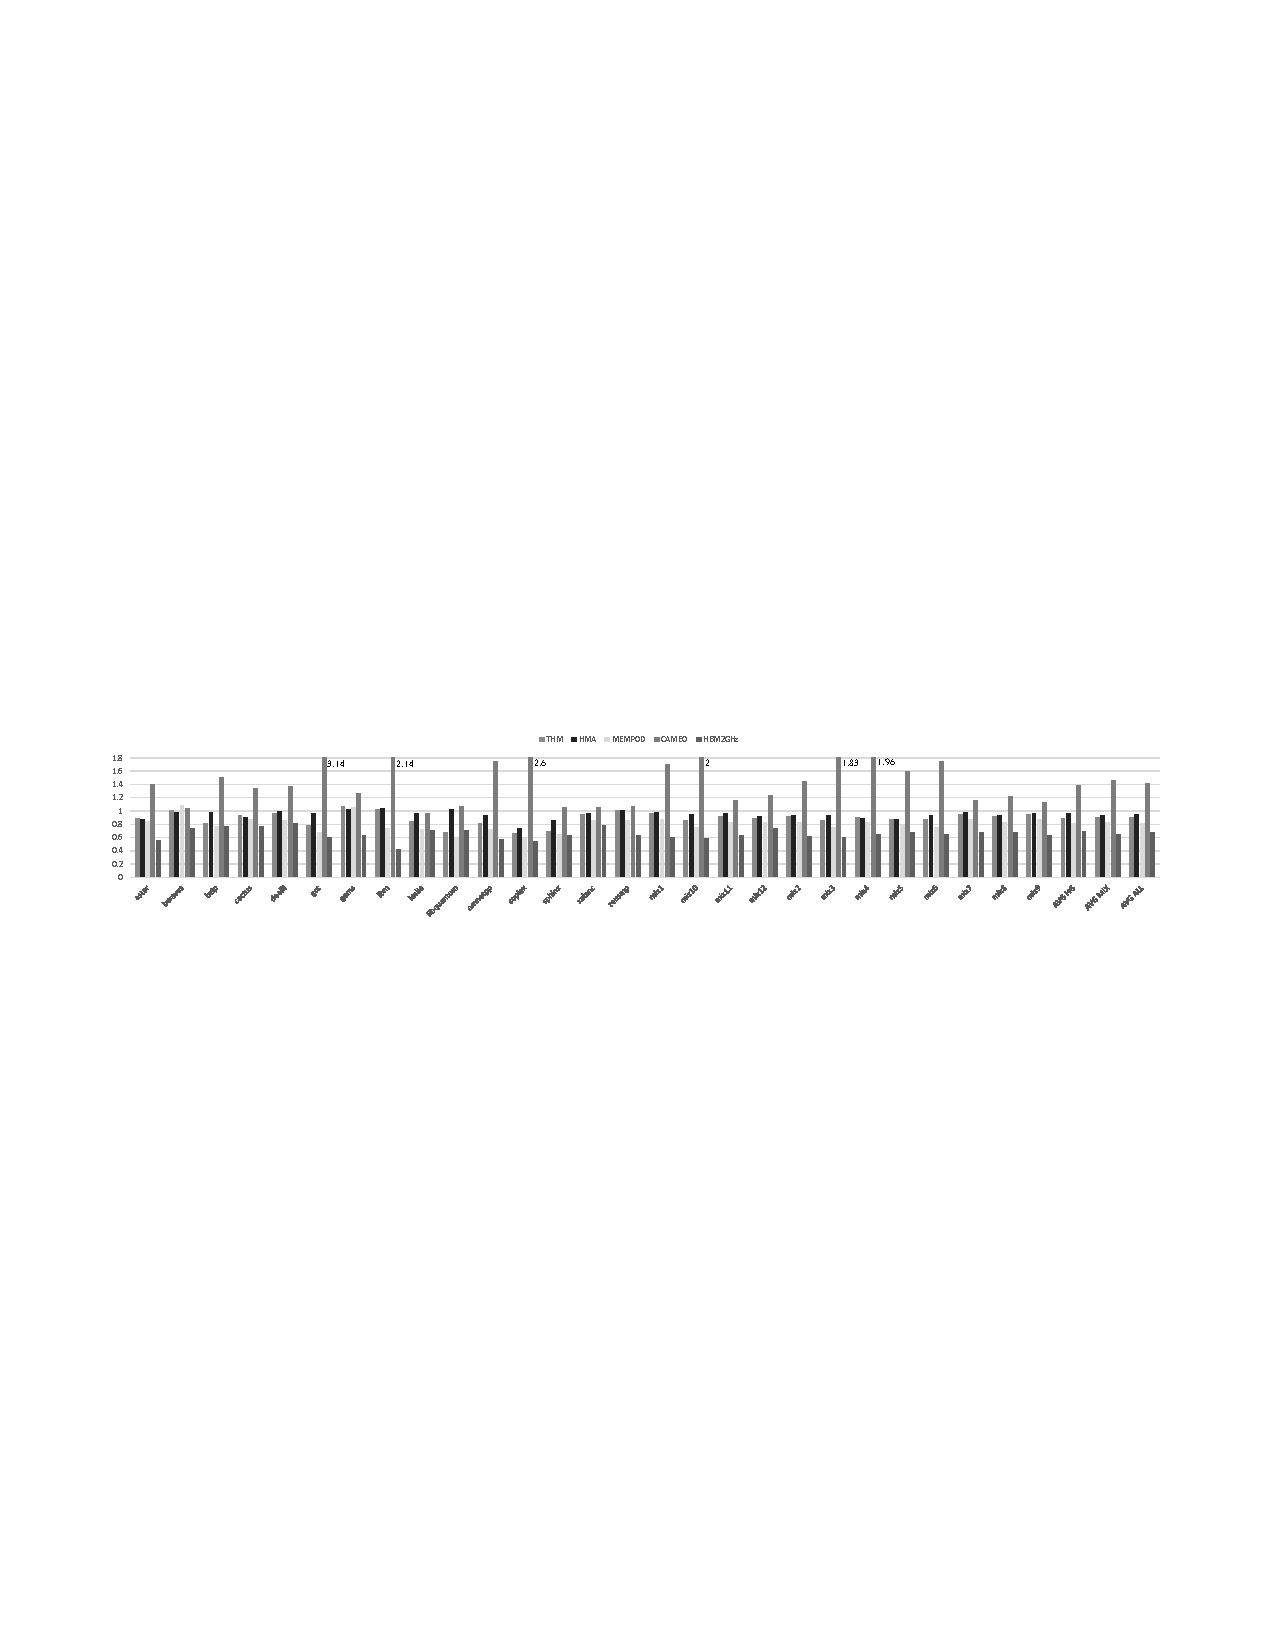
\includegraphics[width=\textwidth]{figures/revised/old/comparison_no_cache.pdf}
  \caption{Performance Comparison: AMMAT is normalized to a hybrid memory without any migration mechanism.}
  \label{fig:performance}
\end{figure*}

Figure \ref{fig:performance} presents a performance comparison of MemPod, HMA, THM, CAMEO and a configuration with 9GBs of on-chip HBM memory, normalized to the performance of a hybrid memory configuration without migration capabilities. We evaluated all mechanisms with caching disabled. 

Based on the results we derive some interesting observations:
\begin{itemize}[leftmargin=0.4cm]
\setlength\itemsep{0em}
	\item MemPod outperforms the state-of-the-art competitors in the majority of our workloads, and in several cases scoring very close to an HBM-only configuration. 
	\item On average, CAMEO reports AMMAT degradation by 41\% over the no-migration scheme. The negative impact is caused by our high slow:fast memory capacity ratio leading to intra-segment conflicts. Larger segments also counteract the application's spatial locality benefits, causing a ping-pong effect. From our experiments, we observe CAMEO to be the leading mechanism regarding the amount of data moved between memories, moving 3.9GB of data on average per 8-core experiment. For comparison purposes, MemPod moved 3GB on average, however migration traffic was divided between Pods, resulting in 790MB per Pod. THM moved 865MB on average and finally HMA moved 578MB due to its large intervals. We also frequently observed redundant migrations with CAMEO, where a line is evicted shortly after migration without being touched in the time it spent residing in fast memory. Optimizations such as intellingent line allocation to segments can significantly improve CAMEO's performance and reduce intra-segment conflicts, however to maintain a fair evaluation, CAMEO is evaluated under the same memory organization as the rest of the mechanisms.\remark {A.P.: Should we make this a subsection on its own?}
	\item On average MemPod reports 21\% higher AMMAT than HBM-only, while THM and HMA report 33\% and 40\% respectively.
	
	\item In some workloads migration overall is harmful to performance, 
as observed with the gems and bwaves workload, where a no-migration scheme reports 
higher performance (lower AMMAT). We observe that in those cases, MemPod leads to deteriorated performance compared to the other mechanisms. However, in the cases of lbm and zeusmp, 
MemPod increases performance, while THM, HMA and CAMEO report higher AMMAT than the no-migration scheme.

	\item HMA and MemPod outperform HBM-only when executing the libquantum experiment. In the case of libquantum, the working set size fits entirely in our fast memory. As a result, after some migrations, the entire working set will be present in HBM.  With an HBM-only system and no migrations, pages
are inserted sequentially by address.  In a migration-based system, 
simultaneously-hot pages are inserted together after each epoch.  As the
DRAM row buffer is bigger than a page, we find that the co-location of
simultaneously-hot pages increases row buffer hit rate from 7\% (HBM only)
to 90\% (MemPod), with 87\% of those taking place in fast memory.  HMA also sees an improvement in row buffer hit rate. THM and CAMEO cannot take advantage of the small footprint due to their restricted migration flexibility (only one hot page/line per segment can reside in fast memory).
\remark{Don't know how to explain THM, but the effect is smaller -- what is
the row buffer hit rate?\\A.P.: THM's results were wrong. The updated results and graph show that it doesn't outperform HBM.}
%However, correct timing is the driving factor behind this impressive performance increase. Our results show the row-buffer hit ratio to be \TODO{??x} times higher than the HBM-only memory system (and random page assignment). Apparently, page migrations resulted in an in-HBM page order that increases page hits and exploits a much higher degree of memory parallelism from the application. This result could be further explored and intentionally recreated in some future work.
\end{itemize}

\subsubsection{Caching Effect}
\ignore{
\begin{figure}
  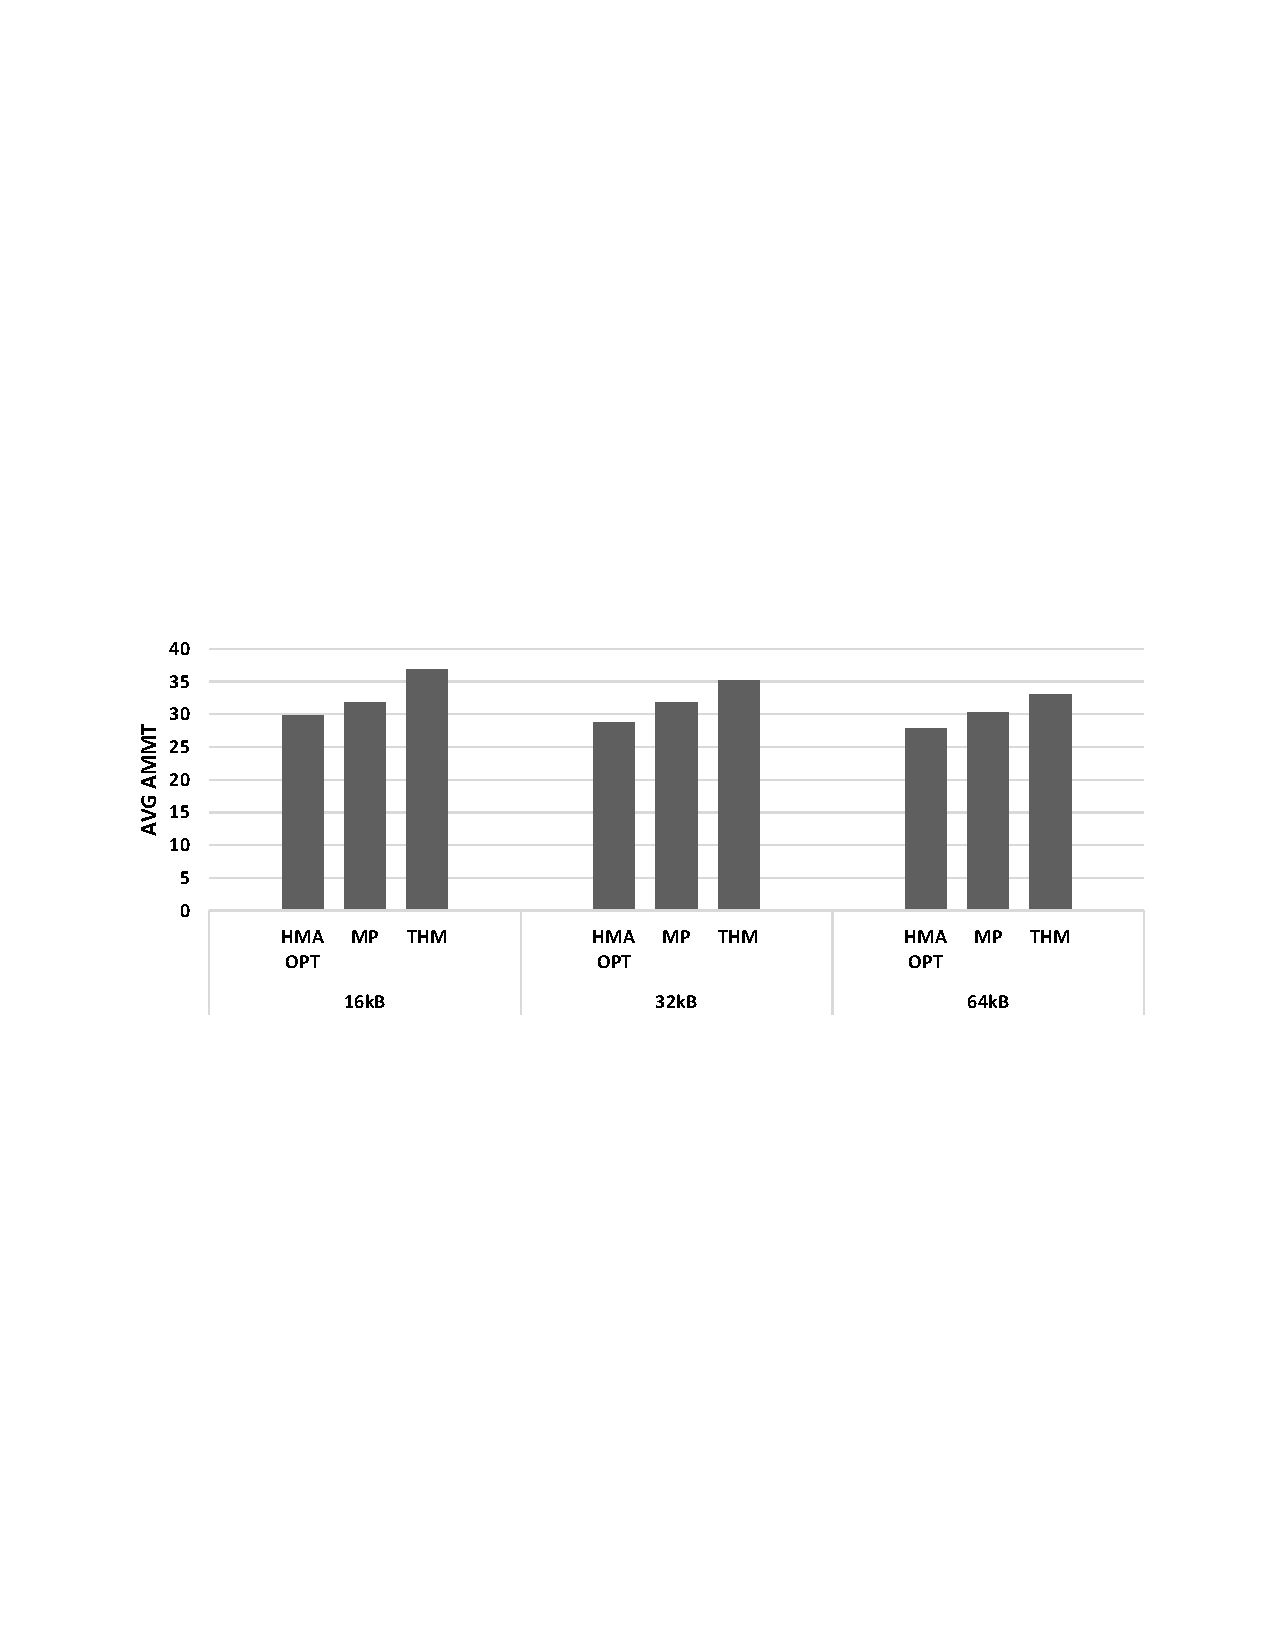
\includegraphics[width=0.46\textwidth]{figures/cache_impact.pdf}
  \caption{Cache Impact. AMMAT normalized to stock TLM (no migrations)}
  \label{fig:cache}
\end{figure}

\remark{A.P.: I don't have CAMEO results with caching yet. Not sure if it will be ready on time but I'm working on it.}

\remark{A.P.: Need to change the structure of this section due to issues with results.}


Migration mechanisms will be forced to include a cache as activity tracking and remap table structures are too large to store on-chip. The use of a cache will unavoidably hinder performance. In this experiment we evaluate the impact of a cache on each mechanism's performance. As described in Section \ref{sec:Architecture}, each mechanism has different cache requirements. THM caches its counters and remap table together with its SRT structure. HMA has no need for a remap table but has high storage requirements for its counting mechanism. MemPod must cache only its remap table as MEA counters will be on chip. We simulated each mechanism with 16, 32 and 64 KB of cache. For MemPod, the available cache capacity was divided equally over four Pods. All mechanisms use the stacked memory as backing store for their tracking information.

HMA's design further complicates this study, as sorting all activity counters at each epoch is performed by the OS, utilizing the cpu's cache instead of the dedicated migration cache. In our results, we present ``HMA-OPT'', an HMA flavor that does not take into account any penalties for OS interrupts, TLB shootdowns, Page Table (PT) updates, walks and misses, or sorting of the large
pool of counters.
We also do not model the application-level effects of starting with a cold TLB after each interval.

Figure \ref{fig:cache} shows our results obtained by taking the average AMMAT from all our workloads for each mechanism. HMA-OPT reports the lowest AMMAT, albeit unrealistic and MemPod outperforms every other mechanism regardless of the cache size. MemPod outperforms THM by 9\% with a 64kB cache, while HMA-OPT outperforms MemPod by 9\%.
}

Migration mechanisms will be forced to include a cache as activity tracking and remap table structures are too large to store on-chip. The use of a cache will unavoidably hinder performance. As described in Section \ref{sec:Architecture}, each mechanism has different cache requirements. THM caches its counters and remap table together with its SRT structure. HMA has no need for a remap table but has high storage requirements for its counting mechanism. MemPod must cache only its remap table as MEA counters will be on chip. 

In this experiment we evaluate the impact of a cache on MemPod's performance. We simulated the optimal MemPod configuration identified over the course of this section with 16, 32 and 64 KB of cache. The available cache capacity was divided equally over four Pods. We implemented MemPod's caching logic to use the stacked memory as backing store, leading to 2.8MBs per Pod to be dedicated for this purpose for an overall 1\% reduction of the available stacked memory capacity.

In our implementation, each cache miss injects a read request to retrieve missing data. Since all of MemPod's cache misses will occur due to Remap Table updates or lookups it becomes a blocking request for the affected Pod. All incoming traffic needs to be delayed until the missing data is retrieved. In-flight requests are not affected by incoming cache misses. Each Pod operates (and blocks) independently allowing other Pods to continue servicing incoming traffic.

\begin{figure}
  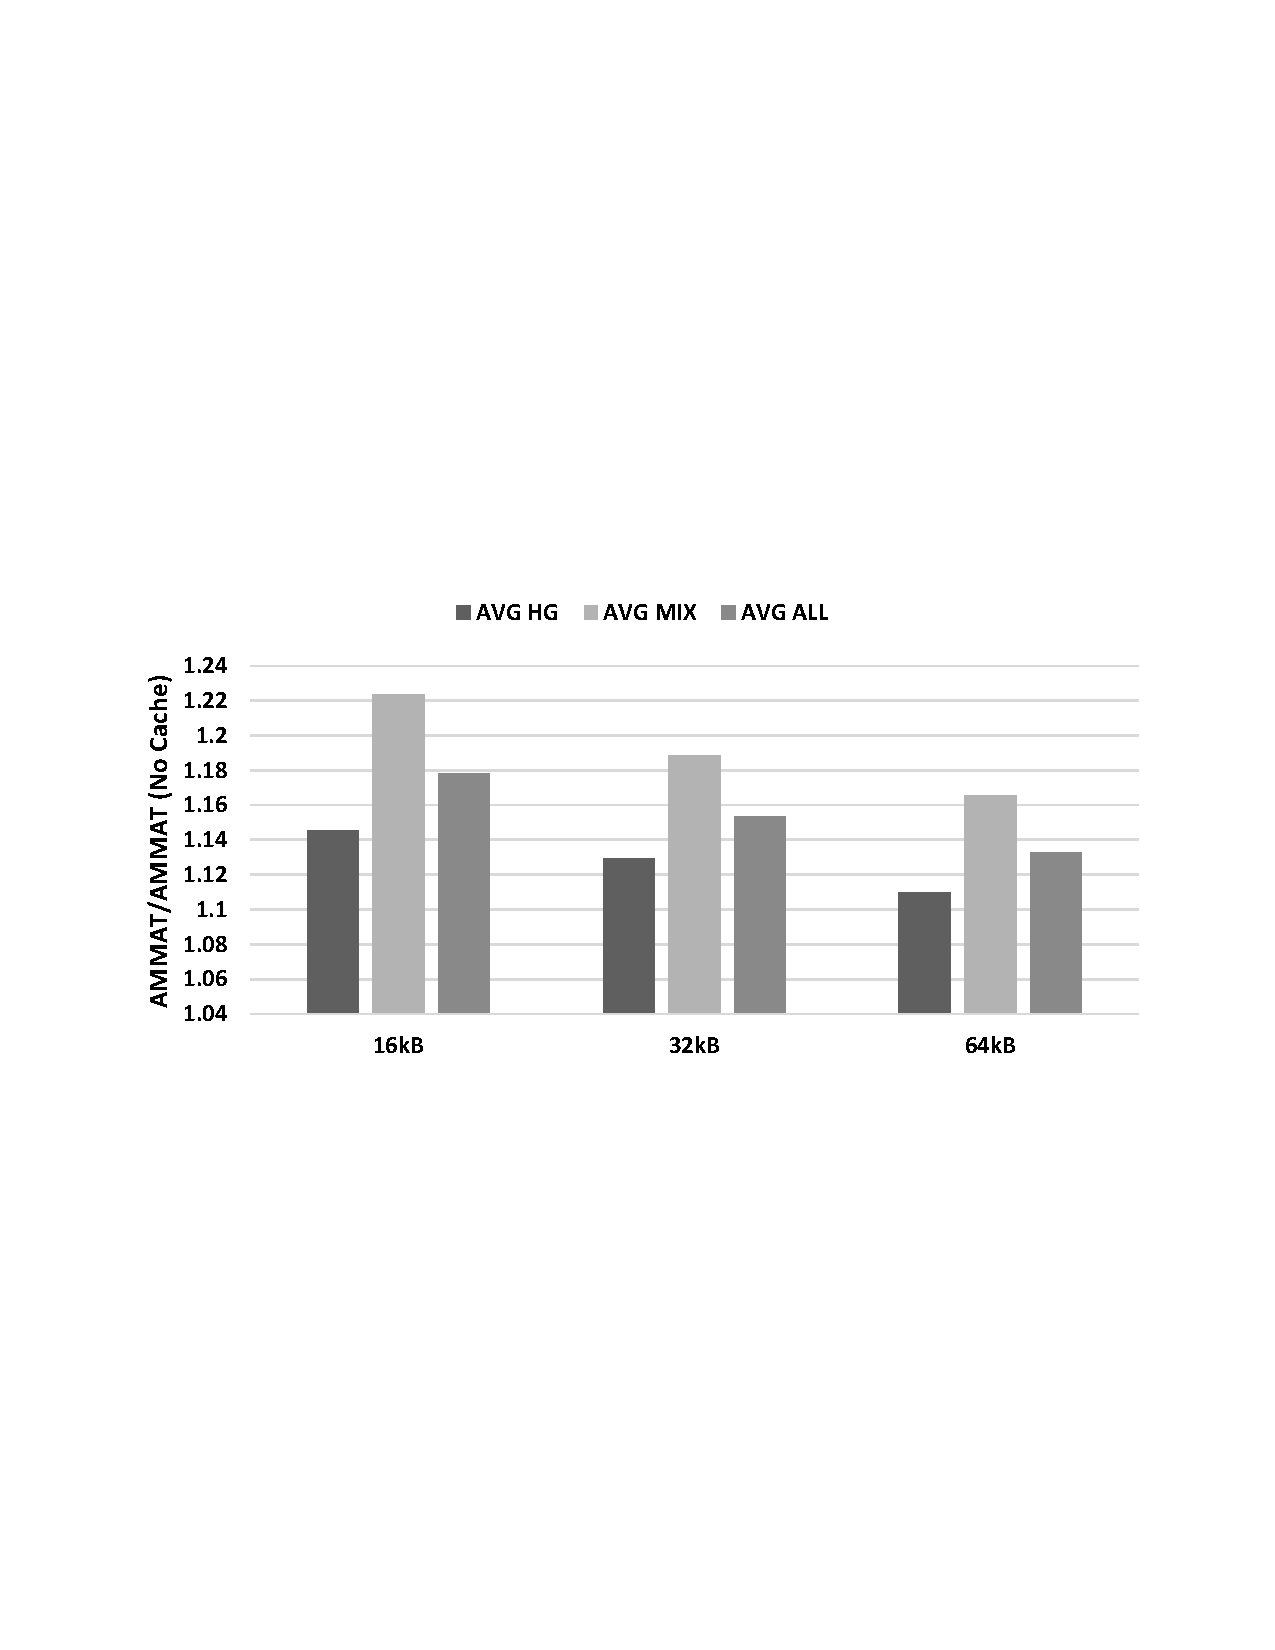
\includegraphics[width=0.46\textwidth]{figures/revised/old/cache_impact.pdf}
  \caption{Cache Impact. AMMAT normalized to stock MemPod (no cache)}
  \label{fig:cache_impact}
\end{figure}

\begin{figure}
  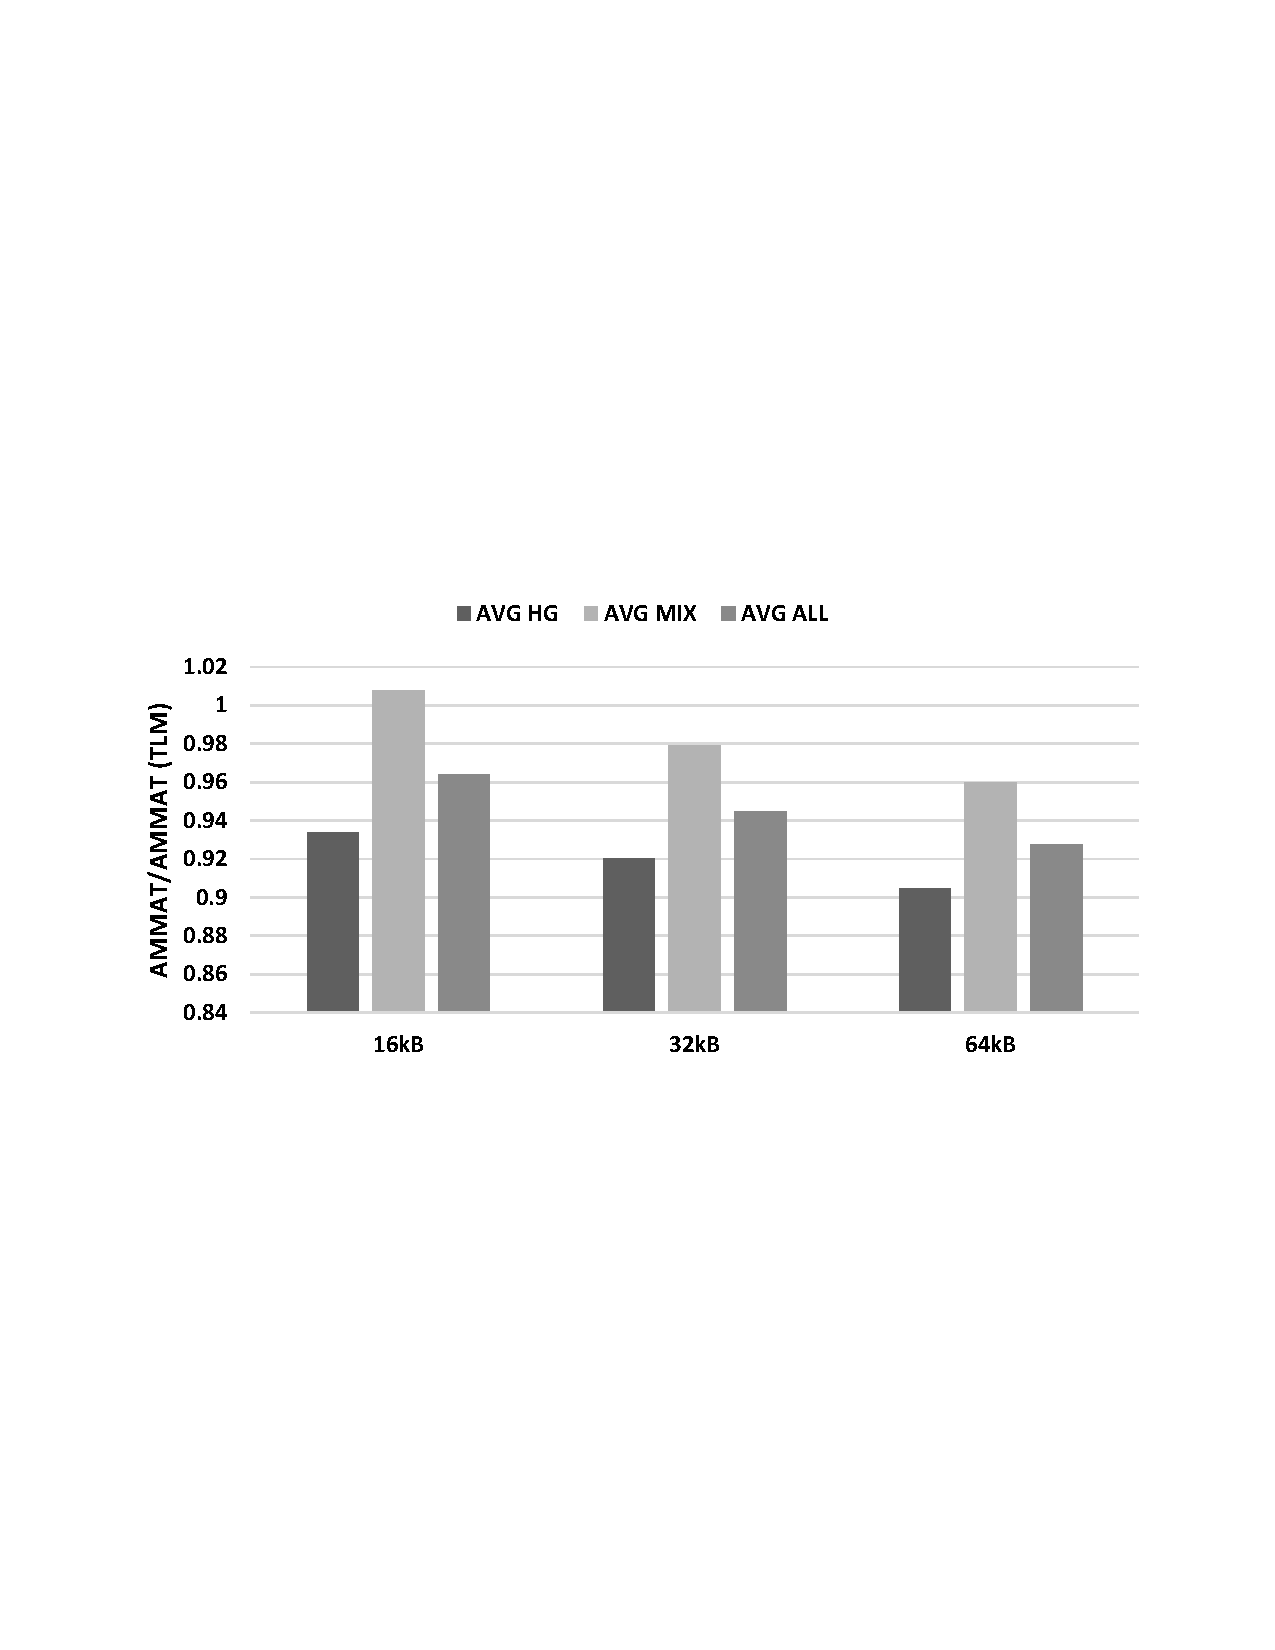
\includegraphics[width=0.46\textwidth]{figures/revised/old/cache_norm_tlm.pdf}
  \caption{Cache Impact. AMMAT normalized to stock TLM (no migrations)}
  \label{fig:cache_norm_tlm}
\end{figure}

Figures \ref{fig:cache_impact} and \ref{fig:cache_norm_tlm} show our results obtained by taking the average AMMAT from all our workloads for each cache size. Figure \ref{fig:cache_impact} shows the obtained average AMMAT normalized to MemPod's performance without a cache. For 16, 32 and 64kB of cache, the impact on MemPod's performance is 18, 15 and 13\% respectively. Figure \ref{fig:cache_norm_tlm} shows our results normalized to a two-level memory configuration without any migration mechanism. With 16, 32 and 64kB of cache, MemPod reports 3.6, 5.6 and 7.3\% AMMAT improvement.

The cache impact is significantly high mainly due to the blocking nature of cache misses. However, a less conservative design could reduce this effect by allowing incoming requests to proceed if they do not depend on any missing information, at some hardware cost. Better cache organization could also help alleviate the issue.

\subsubsection{Scalability}

\begin{figure}
  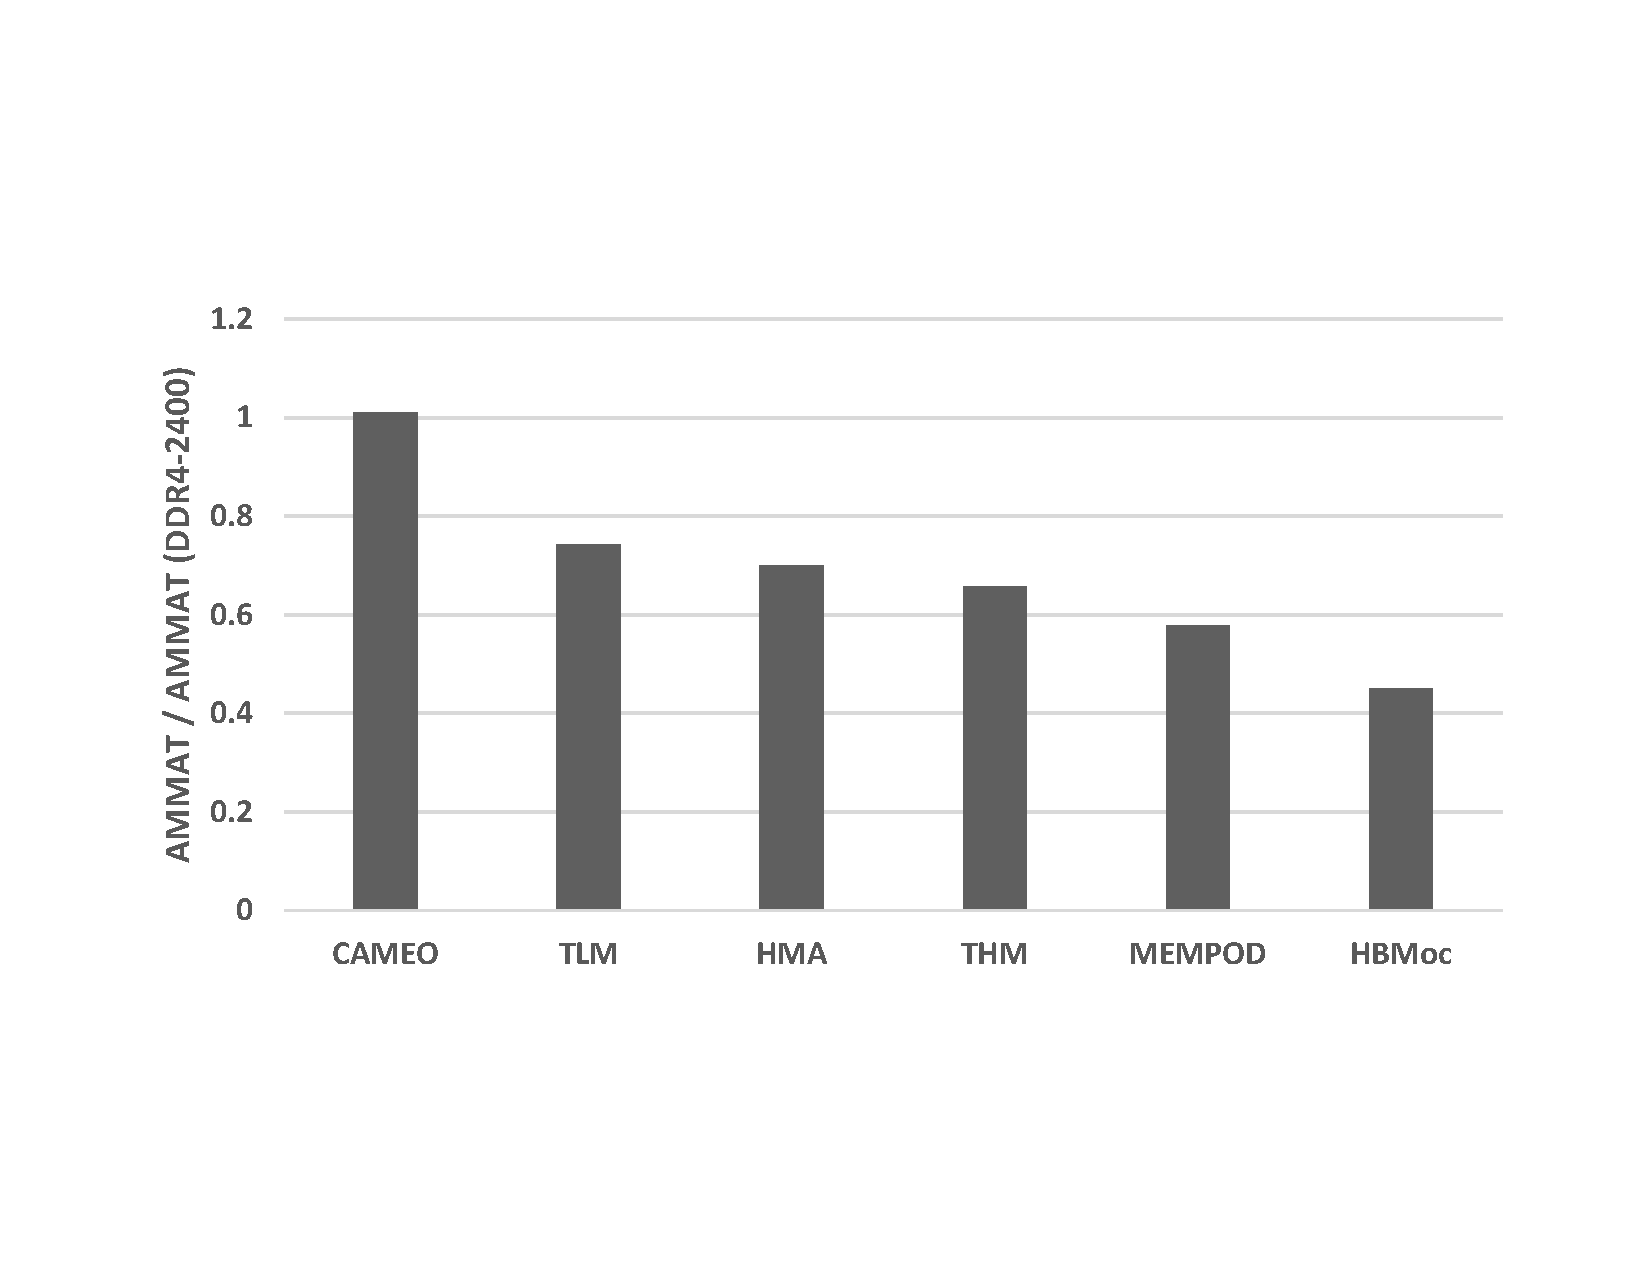
\includegraphics[width=0.46\textwidth]{figures/revised/old/scalability_speed.pdf}
  \caption{Scalability to faster memories. AMMAT normalized to a DDR4-only memory.}
  \label{fig:scalability}
\end{figure}

MemPod is designed to be scalable with future technology.  If we grow memory
sizes by increasing the number of pods, the size of the remap table and the 
size of the MEA counters will remain constant (per pod, and thus per memory
page) if the memory per pod remains constant.  If instead we increase
memory capacity per pod, the size of the remap table (per memory page)
will go up only with the log of the per-pod memory. If we choose to scale
the number of counters with the size of memory per pod, it will go up
similarly; however, if we do not scale up the counters at the same rate
(e.g., four times the memory, but double the counters), then the cost
of the counters (per memory page) will go down.

Additionally, the memory traffic caused by migrations will remain distributed
and off the primary processor interconnect.

We also expect the latency differential between main memory levels to 
continue to grow.  This will happen as 3D memory parts mature, and as
we integrate new memory technologies into the system (e.g. hybrid
volatile and non-volatile memory systems).
To examine this, we model a system where both the 3D DRAM and the DDR memory
are faster, but the 3D DRAM is accelerated further resulting in a higher
latency ratio between the two. 
In particular, we simulate a 4GHz HBM as our stacked memory and a DDR4-2400 as our off-chip memory. 
We assume no cacheing effects in this experiment.
Figure \ref{fig:scalability} shows our AMMAT results, normalized to a configuration with 9GBs of off-chip DDR4-2400. The label ``HBMoc'' shows a 9GB configuration with overclocked HBM only. We first observe that CAMEO now reports a 1\% AMMAT degradation. The increase in speed differential between stacked and off-chip memory appears to be beneficial, however we can still observe the impacts of intra-segment conflicts. Compared to a configuration with no migration support (TLM), HMA improves AMMAT by 6\%, THM by 12\% and MemPod by 22\%. The overclocked HBM-only configuration is 40\% faster compared to TLM.

\ignore{
We first observe that HMA-OPT due to its high number of 
migrations and low prediction accuracy increases AMMAT by 8\% compared to a 
Two-Level Memory without migration (TLM). THM and MemPod reduce AMMAT by 13\% and 24\% respectively, compared to TLM. With this memory configuration, MemPod 
reports AMMAT improvements of 42\% over HMA-OPT, and 15\% over THM. 
}


% !TEX root = ../MemPod.tex
\section{Conclusions}
\label{sec:Conclusions}

MemPod is a scalable, modular and efficient dynamic memory management mechanism. Our analysis demonstrates significant gains compared to state-of-the-art proposals. The modular design achieved with the use of Pods allows for a more scalable migration mechanism while at the same time enforcing small limitations on migration opportunities.

MemPod uses MEA counters to track page access activity and identify hot
pages.  They are dramatically smaller than prior tracking mechanisms
while capturing both activity counts and temporal recency in a way that
provides a more effective prediction of future page access.

\remark{give some numbers for overall performance gains.}


\remark{No reason to describe future work.}
%\TODO{Not sure what to keep/remove here. I'll think a little more about it.}
%In addition, MemPod leaves a lot to be investigated in future work. We intend to focus on extending our design to support even more complex memory configurations, with the addition of non-volatile memory which adds a reliability aspect. Ordering of migrations could result to incredible increase in performance, as demonstrated in experiment ?? and libquantum, allowing for future research. MemPod could also be used to accommodate memory scheduling mechanisms by utilizing its internal structures, or on the other hand, we could focus on ``Pod-aware'' memory scheduling.


%\bstctlcite{bstctl:etal, bstctl:nodash, bstctl:simpurl}
%\bibliographystyle{IEEEtranS}
\bibliographystyle{ieeetr}
\bibliography{references}

\end{document}
